
\documentclass{ltjsreport}
% 数理系
\usepackage{amsmath,amsbsy,amssymb}
\usepackage{mathtools}
\usepackage{physics2}
\usepackage{siunitx}
\mathtoolsset{showonlyrefs=true}
% 画像
%\usepackage[draft]{graphicx}
\usepackage{graphicx}
% ロゴ関係
\usepackage{bxtexlogo}
\bxtexlogoimport{*,**}
% Hオプションを使いたいので読み込む
\usepackage{here}
% ソースコードを表示するのに読み込む
\usepackage{listings} % 用例: \lstinputlisting[caption=sqrt.cpp,style=c++]{./sqrt.cpp}
% シンタックスハイライトのため
\usepackage{xcolor}
% url挿入のため
\usepackage{url}
% 枠のため
\usepackage{ascmac}
% xcolorの色定義
\definecolor{solarized@base03}{HTML}{002B36}
\definecolor{solarized@base02}{HTML}{073642}
\definecolor{solarized@base01}{HTML}{586e75}
\definecolor{solarized@base00}{HTML}{657b83}
\definecolor{solarized@base0}{HTML}{839496}
\definecolor{solarized@base1}{HTML}{93a1a1}
\definecolor{solarized@base2}{HTML}{EEE8D5}
\definecolor{solarized@base3}{HTML}{FDF6E3}
\definecolor{solarized@yellow}{HTML}{B58900}
\definecolor{solarized@orange}{HTML}{CB4B16}
\definecolor{solarized@red}{HTML}{DC322F}
\definecolor{solarized@magenta}{HTML}{D33682}
\definecolor{solarized@violet}{HTML}{6C71C4}
\definecolor{solarized@blue}{HTML}{268BD2}
\definecolor{solarized@cyan}{HTML}{2AA198}
\definecolor{solarized@green}{HTML}{859900}
% listingsのスタイル定義
\lstdefinestyle{c}{
  language=c,
  numbers=left,
}
\lstdefinestyle{c++}{
  language=c++,
  numbers=left,
}
\lstdefinestyle{python}{
  language=python,
  numbers=left,
}
\lstset{
basicstyle=\small\ttfamily\color{solarized@base00},
rulesepcolor=\color{solarized@base03},
numberstyle=\scriptsize\color{solarized@base01},
keywordstyle=\color{solarized@blue},
stringstyle=\color{solarized@cyan}\ttfamily,
commentstyle=\color{solarized@base01},
emphstyle=\color{solarized@red},
backgroundcolor=\color{solarized@base3},
sensitive=true,
breaklines=true,
breakatwhitespace=true,
framerule=0pt,
frame=l,
showstringspaces=false,
tabsize=2,
basewidth={0.57em,0.52em},
}

\title{情報メディア実験Bレポート\\ライントレーサロボットのフルスクラッチ実装}
\author{202111609\\ 仲村 和士}
\date{\today}

\setcounter{tocdepth}{2}

\usepackage{hyperref}

\newcommand{\para}[2]{\frac{#1 #2}{#1 + #2}}
\newcommand{\paral}{/\!/}
\newcommand{\diff}{\mathrm{d}}
\newcommand{\dft}[1]{\frac{\mathrm{d}#1}{\mathrm{d}t}}

\begin{document}
\maketitle



\tableofcontents

\chapter{はじめに}


\section{目的}
本実験では、ライントレーサロボットの制作を通して、電気回路解析、制御工学に関する理論、および実際のソフトウェア、ハードウェアへの応用を学ぶことを目的とする。
ライントレーサロボットは、周囲と明るさの異なるコース線(一般的には黒色または白色)を追従する非常に単純なロボットであり、最もシンプルな制御方法とキットを用いればロボット製作が初めての小学生でも容易に制作が可能なレベルである。しかし、フルスクラッチで設計し、高速で追従させようとすると必要な知識は広範にわたり、難易度は高くなる。本レポートでは、ロボット製作の過程での学習成果、および、実際のロボットの設計、製作方法、評価についてまとめる。

\section{本レポートの構成}
\ref{cha:electric}章では、電気回路解析の基本についての学習成果として、直流回路および交流回路の解析手法をまとめる。

\ref{cha:electric}章の内容は一般的なものであるから、読む時間がない場合は飛ばして次の\ref{cha:hardware}章から読むことを推奨する。
\ref{cha:hardware}章では、実際に走行体に使用したハードウェア設計について部分に分割して示す。
\ref{cha:software}章では、ソフトウェア設計について、システム構成、制御手法および、部分ごとの実装について示す。
これら設計に関する章ではこれから作ろうとする人に向けた解説という体で記述している。
\ref{cha:eval}章では、走行体の評価、振り返り、改善点、感想等について示す。

\chapter{電気回路解析の基本}\label{cha:electric}
\section{概要}
本章では電気回路解析の基本的な方法について学習したことを解説する。
学習には教科書~\cite{ElectricCircuit}を使用した。
ロボットを作るときには、回路設計が必要不可欠である。
正しい知識のもとに回路設計を行えば初歩的なミスによる部品の破壊が減らせるほか、
トラブルが発生したときの原因究明にも回路解析の知識が役に立つ。
もちろん、ここで扱うすべての知識が今回のロボット製作に直ちに役に立つ訳では無い。
たとえば、電気回路解析のメインテーマは直流回路ではなく交流回路であるが、今回のロボット製作で交流回路を利用している人はいないだろう。しかし、直流回路であってもDC-DCコンバーダのように交流に似た理論で動く部品は存在するし、発振器を使用した回路も決して珍しくない。コンデンサはどうだろうか。直流回路にコンデンサは登場しないが、実際に扱う回路は理想的ではないから過渡現象が存在することを忘れてはいけない。
そして、電源基板のような部分には過渡現象を抑えるためにコンデンサが使われているが、それを解析するためには交流回路の知識があったほうが便利である。
一通りの知識を抑えておくことで直接的には関係ないように思われる場面で役に立つことは非常に多い\footnote{学習量が膨大だったため、レポートに書ききれなかったことも多い。交流回路の電力、Quality factor、歪み波交流、過渡現象、磁気結合回路、4端子回路、3相交流回路、分布定数回路など。}。

本章では高校で学習するキルヒホッフの法則を紹介したあと、キルヒホッフの法則よりも楽に早く回路を解析するための手法を紹介し、キルヒホッフの法則からの脱却を図るというコンセプトで電気回路解析の基礎を解説する。



\section{電気回路の導入}
\subsection{導入}
それでは早速始めよう。
まず、電気回路にはどのような構成要素があるだろうか。
非常にシンプルである。基本的には、電源、配線、抵抗という3つの要素しかないと考えて問題ない。
これは直流回路に限らず、交流回路の世界ではコンデンサ、インダクタといった素子が登場するものの、驚くことにこれらの素子は一定の手続きを踏めば抵抗と同じように考えて解くことができるのである。
\footnote{注意点としては、電気回路の世界ではほとんどの場合「線形の回路」のみを扱う。
線形な回路は線形な素子から構成される。少し難しく感じられるが、線形な素子であるかどうか大雑把に判定するな方法としてはオームの法則に従うかどうかを考えれば良い。豆電球のような非オーム抵抗は線形な素子ではない。その他にも、半導体素子であるトランジスタやダイオードなども線形な素子ではない。これらは電子回路の範囲で扱うものである。}

次に、電気回路が解けるとはどのような状態であるだろうか。
多くの場合、既知の素子を接続した回路上で任意の点の電流と、2点間の電圧が求められている状態を指す。
よって、我々は「電流」と「電圧」について正しい理解をする必要がある。

\subsection{電流と電圧}
まずは電圧から考えよう。
電磁気学を学んだ人に説明するなら、「単位電荷に換算した静電気力のポテンシャルエネルギーである電位の2点間の差」「電場を積分して求められる電位の2点間の差」などと言えば十分であるが、
実は、電磁気学を学んでいない人に電圧の概念を正しく理解してもらうのは意外と難しい。
たとえば、中学理科を説明しているトライさんのサイト~\cite{TRY}では、「電圧のイメージは、流れる電子1粒のいきおいのこと」「電流 のイメージは、1秒間に流れる電子の数のこと」とされている。
この文章から電圧と電流の違いがわかるだろうか?
理解している人にとってはこの文章は大きく外してはいないことがわかる。
しかし、勢いが強いと言われれば、電子(電荷)が高速で流れている状態をイメージしやすい。そして電荷のスピードというのはどちらかというと電圧ではなく電流の定義である。やはりよくわからなくなってしまった。

そこで、状況を説明するのに昔から用いられているのが水流のモデルである。これも正しく意味を吟味できていないと大きな誤解を招く諸刃の剣であるが、この考え方では次のように置き換えることができる\footnote{水流モデルには圧力に基づくモデルと高さの差に基づくモデルの二種があり、あまり明確に区別されずに用いられてきたことが文献~\cite{WATER}で考察されている。}。
電源\leftrightarrow 水を上に汲み上げるポンプ、配線\leftrightarrow 水平な水路、抵抗\leftrightarrow 水路中につけた水車、として閉じた水路を形成する。このようにおけば、ポンプで水を持ち上げる高さ$h$に比例して単位時間あたりに水路中のある位置を通過する水の量は増加する。もし、$h=0$であれば水が流れることはない。
同じことが電気回路にも言える。電気回路では、高さにあたるのが電圧、単位時間に水路の断面を通過した水の量が電流、となる。
注意点としては、「高さ」という量は常に2点間の差で決定されていて、1点で絶対的に決定されるわけではないということである。
たとえばポンプで水を5 \si{\m}汲み上げたとき、その基準となっているのは持ち上げる前の位置である。
逆に、ポンプで水を汲み上げたあとの高さを基準の高さ0 \si{\m}とすれば、持ち上げる前の高さは-5 \si{\m}である。
おなじことが電圧にも言えて、電圧が1.5 \si{\V}の電池は負極を基準とすれば正極は1.5 \si{\V}であるが、正極を基準とすれば、負極は-1.5 \si{\V}である\footnote{回路図中では電圧の基準点はGND(グラウンド)と書かれることが多い。}。
電圧と聞くと水圧のように1点で決まるものであると誤解しやすい。そういった誤解をなくすために、電磁気学では電圧と同じ意味で「電位差」という言葉がよく使われることを覚えておくとよいだろう\footnote{電位と電圧は似た使われ方をするので少々わかりにくいことがある。気持ち的には、明示的には書かれていないが、どこかに基準があることを前提としてある1点の電気的な高さを述べたいときには電位と表し、2点を明示してその電気的な高さの差について述べているときには電圧と書く。}。

次に電流について考えよう。
水流モデルを考えれば、水流は(水流) = (通過水量)/(経過時間)で表現できる。
同様に電流を表現すれば、
\[  
  I(電流) = Q(電荷の通過量)/t(経過時間)
  \]
となる。
これを拡張して微小時間でも同様の性質が成り立つと考えれば、
\[
  i(t) = \frac{dq(t)}{dt}
\]
が成り立つ。

では抵抗はどのような装置であると考えられるか。
抵抗はエネルギーを別の種類のエネルギーへと変換して取り出す装置である。
水車は水の位置エネルギーを主に運動エネルギーへと変換する。
同様に、電気回路中の抵抗は電気エネルギーを主に熱エネルギーへと変換する装置である。

\subsection{オームの法則}
図\ref{fig:ohm}ような単純な回路を考える。
水流モデルと同様に、電気回路でも与えた電圧$E$に比例して電流$I$は増加する。このとき、以下の式が成り立つ。

\begin{figure}[bt]
  \centering
  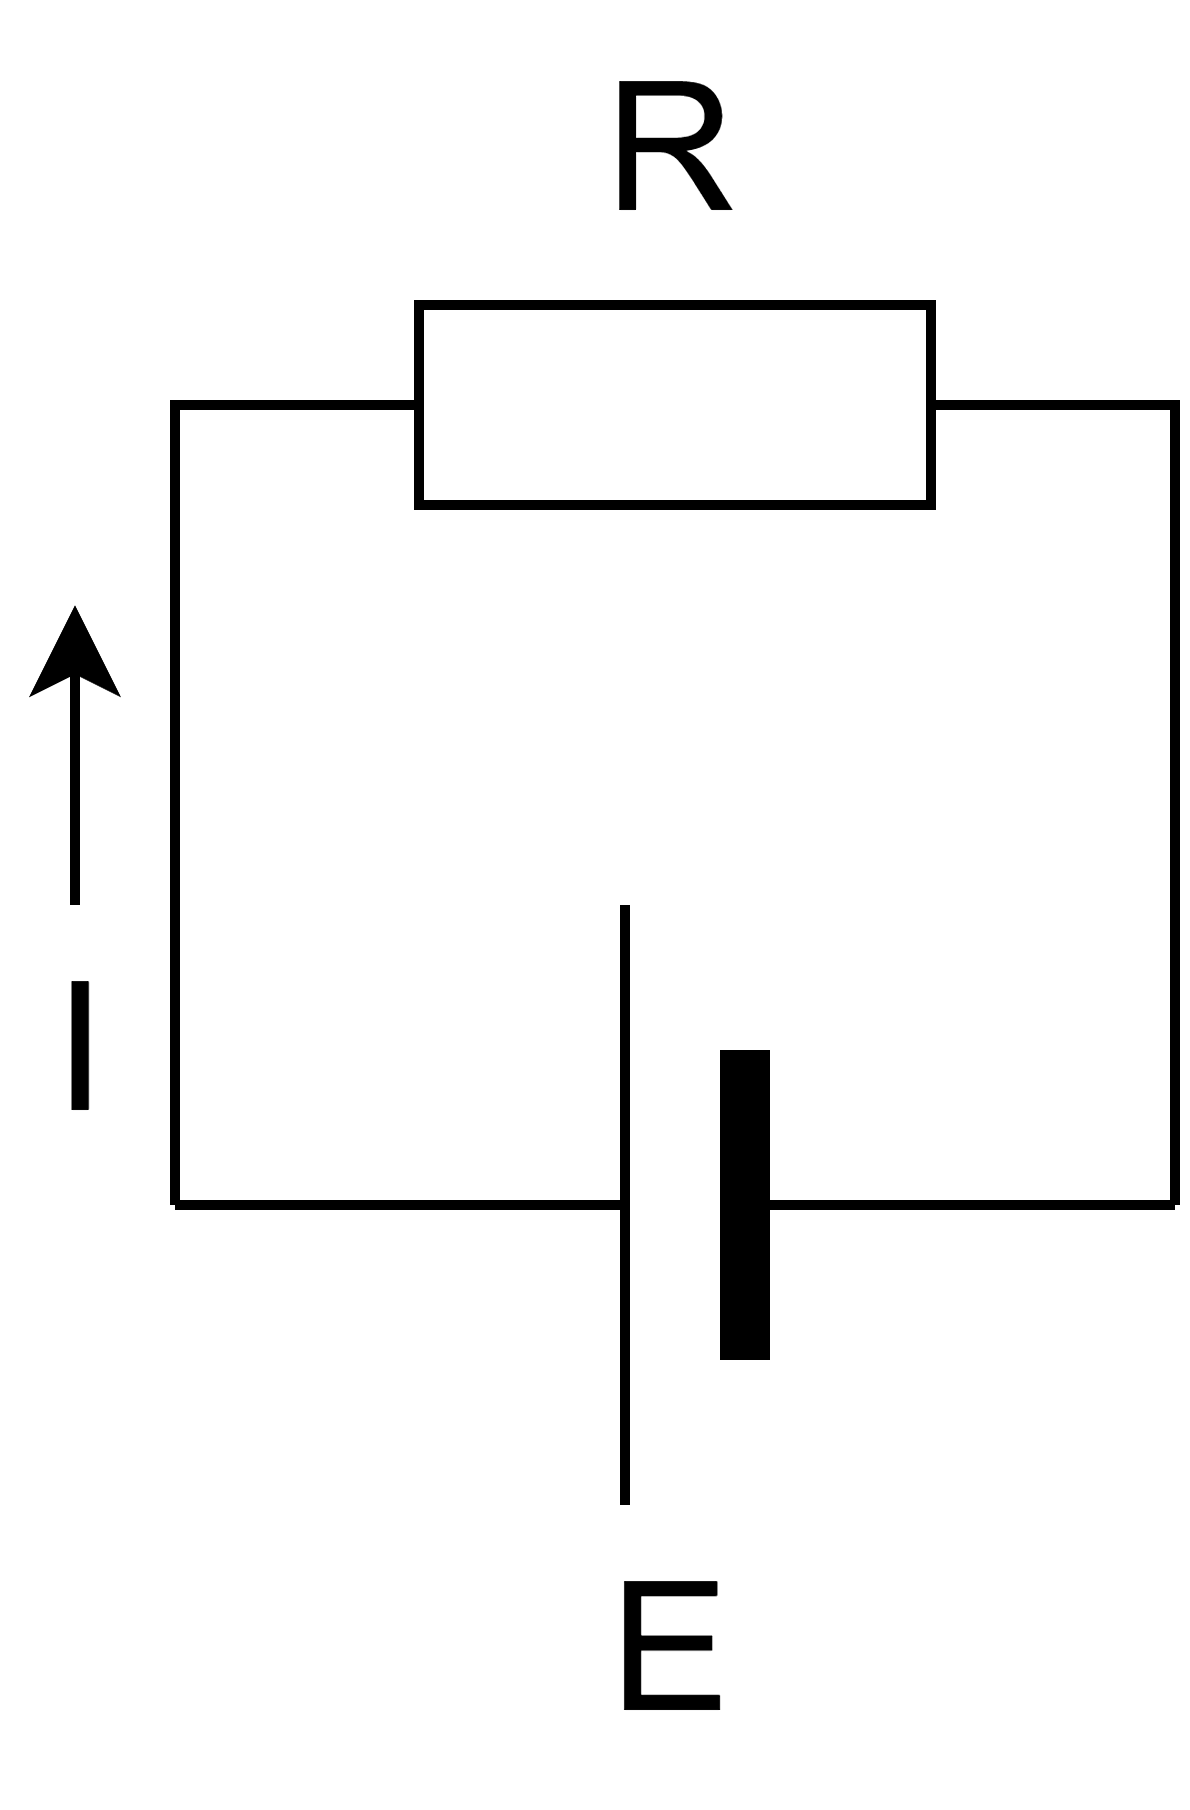
\includegraphics[keepaspectratio, scale=0.07]
       {img/ohm.drawio.png}
  \caption{}
  \label{fig:ohm}
 \end{figure}
\begin{equation}
  E = RI \label{eq:ohm}
\end{equation}

この係数Rが抵抗である。
同じ電圧ならば抵抗が大きいと電流は小さくなるため、抵抗は電流の流れにくさを表す。
通常、Rは時間によらず一定であるとみなして解析するが、実際の抵抗は温度変化による抵抗値の変動があるので注意する必要がある。
Rが一定であるとみなせるとき電圧と電流は比例し、このような関係は線形性とよばれる。
電気回路の諸定理の中には線形性を満たすものにのみ適用できるものも多いから適用範囲に注意しなければならない。



また、抵抗の逆数$G = 1/R$を用いると、オームの法則は以下のように変形できる。

\begin{equation}
  I = GE
\end{equation}

この$G$をコンダクタンスとよび、電流の流れやすさを表す。

\subsection{理想電源}

\subsubsection{理想電圧源}
回路の状態によらず、常に負極と正極の間の電圧が一定であり、一切の内部抵抗がない電源装置を理想電圧源と呼ぶ。

実際の電源装置は理想電源ではない。
たとえば、生活の中で身近な直流電源装置として、電池があげられる。
電池は利用しているとだんだんと消耗し、両端の電圧が下がっていく。
また、瞬間的に大きい電流が流れたときに両端の電圧が下がることがあり、やはり一定とは見なせない。
そして、電池は内部抵抗が存在するため純粋に電源の機能だけとは見なせないのである。

\subsubsection{理想電流源}
回路の状態によらず、常に接続部分に一定の電流を流す電源装置を理想電流源と呼ぶ。

電圧と電流の因果律を考えれば、電圧があることが原因で電流が生じるから、電流源はより現実の電源装置からは離れた概念である。
しかし、後述するように電源の等価変換を考えることにより回路解析では有用な場面がある。

\subsubsection{現実の電源の等価電源} \label{sec:source}
先に述べたように電池のような現実の電源は理想電源ではない。
しかし、内部抵抗を考慮することで、より現実に近い電源モデルを考えることができる。
図\ref{fig:real_battery}のように、電圧源の場合は理想電圧源$E$と直列に抵抗$R_{in}$を挿入し、電流源の場合は理想電流源$I$と並列に抵抗$R_{in}$を挿入することで、内部抵抗を考慮した電源モデルとなる。
\begin{figure}[tb]
  \centering
  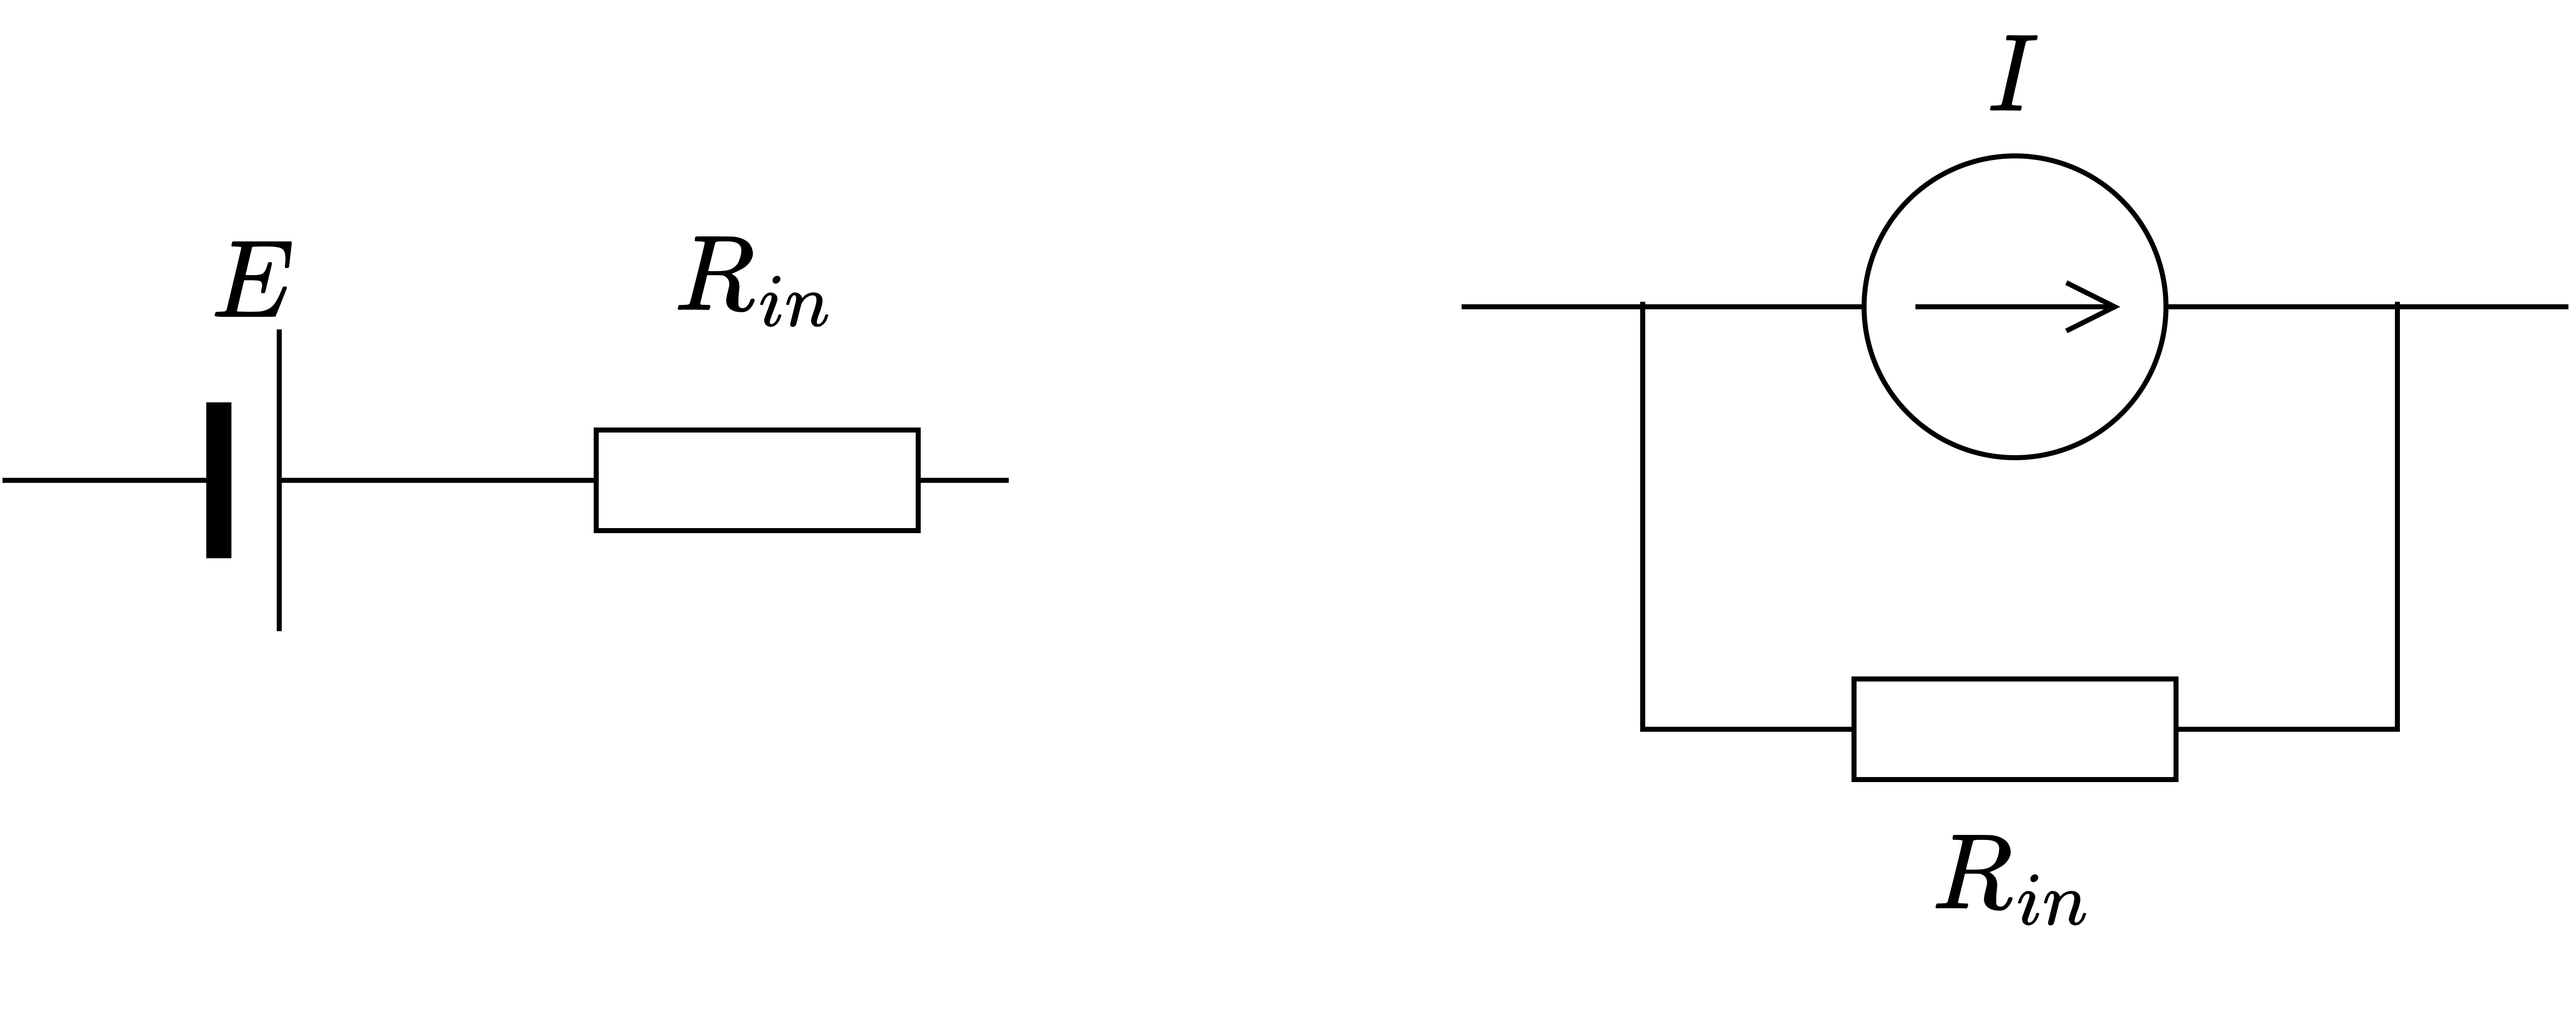
\includegraphics[keepaspectratio, scale=0.07]
       {img/real_battery.drawio.png}
  \caption{現実の電源の等価電圧源と等価電流源}
  \label{fig:real_battery}
 \end{figure}




\subsection{電力}

電気が単位時間に行う仕事、すなわち、仕事率のことを電力とよぶ。ある抵抗Rで消費される電力$P$は、抵抗にかかる電圧$V$と抵抗に流れる電流$I$を用いて、以下のように表される。
\[
  P = VI = RI^2 = V^2/R
\]
電力の単位はW (ワット) であり、$[\si{W}] = [\si{J}]/[\si{s}]$である。



\section{直流回路の解析}

\subsection{電圧上昇と電圧降下}
オームの法則を用いることで、単純な回路については解析することができる。

ここで、回路解析のうえで重要な概念である「電圧上昇」と「電圧降下」の概念について説明する。
図\ref{fig:voltup_down}のような回路を考える。
ただし電圧の矢印は電位の低い方から高い方へ向けて書くことと約束する。
この回路において、$1^\prime$を基準とした各端子の電位を考える。電流の向きに沿って考えると、まず、$1^\prime$から$1$へ移動する間の電源で$E$の電圧上昇があるから$1$の電位は$E$である。
次に、$1$から$2$に移動する過程では抵抗$R_1$により、$V_1=R_1I$の電圧降下がある。
そして、$2$から$1^\prime$に戻る過程で抵抗$R_2$により、$V_2=R_2I$の電圧降下がある。
これらから方程式を導くと、
\begin{align} 
  E &= V_1+V_2\\ \label{eq:ohm2}
    &= R_1I +R_2I
\end{align}
となる。
つまり、
\[
  (電圧上昇の和) = (電圧降下の和)
\]
あるいは、
\[
  (電圧上昇の和)-(電圧降下の和) =0
\]
が成り立つ。

次に、同じ意味であるが他の見方を示そう。
図\ref{fig:voltup_down}を見ると、電源電圧$E$は電流の方向に沿って上昇している一方で、抵抗$R_1, R_2$にかかる電圧は電流と逆の向きに沿って上昇していることがわかる。このような状況は、抵抗が「逆向きに接続された電源」のように振る舞っていると解釈することができる。この逆向きの電圧を「逆起電力」と呼ぶことがある\footnote{抵抗による逆起電力という言葉は交流回路で登場するインダクタ(コイル)による逆起電力と本質的に別の仕組みであるため、混同を防ぐため使わない方がよいという意見もある。回路方程式を立てるうえでは両者とも電流の逆向きに沿って正の起電力があると見なせるので同じ手続きで問題ない。}。
これを式にすれば、
\[
  (電源による起電力の和) = (逆起電力の和)
\]
となり、これは前に示した電圧上昇、電圧降下によるモデルと等価な式である。

% ここで、式\eqref{eq:ohm2}と式\eqref{eq:ohm}を比較すると、2つの回路は直列に接続された$R_1$と$R_2$を$R$に置き換えたものであるから、
% $R_1$と$R_2$を直列に合成した抵抗$R$は$R=R_1+R_2$の関係があることが導かれる。


\begin{figure}[tb]
  \centering
  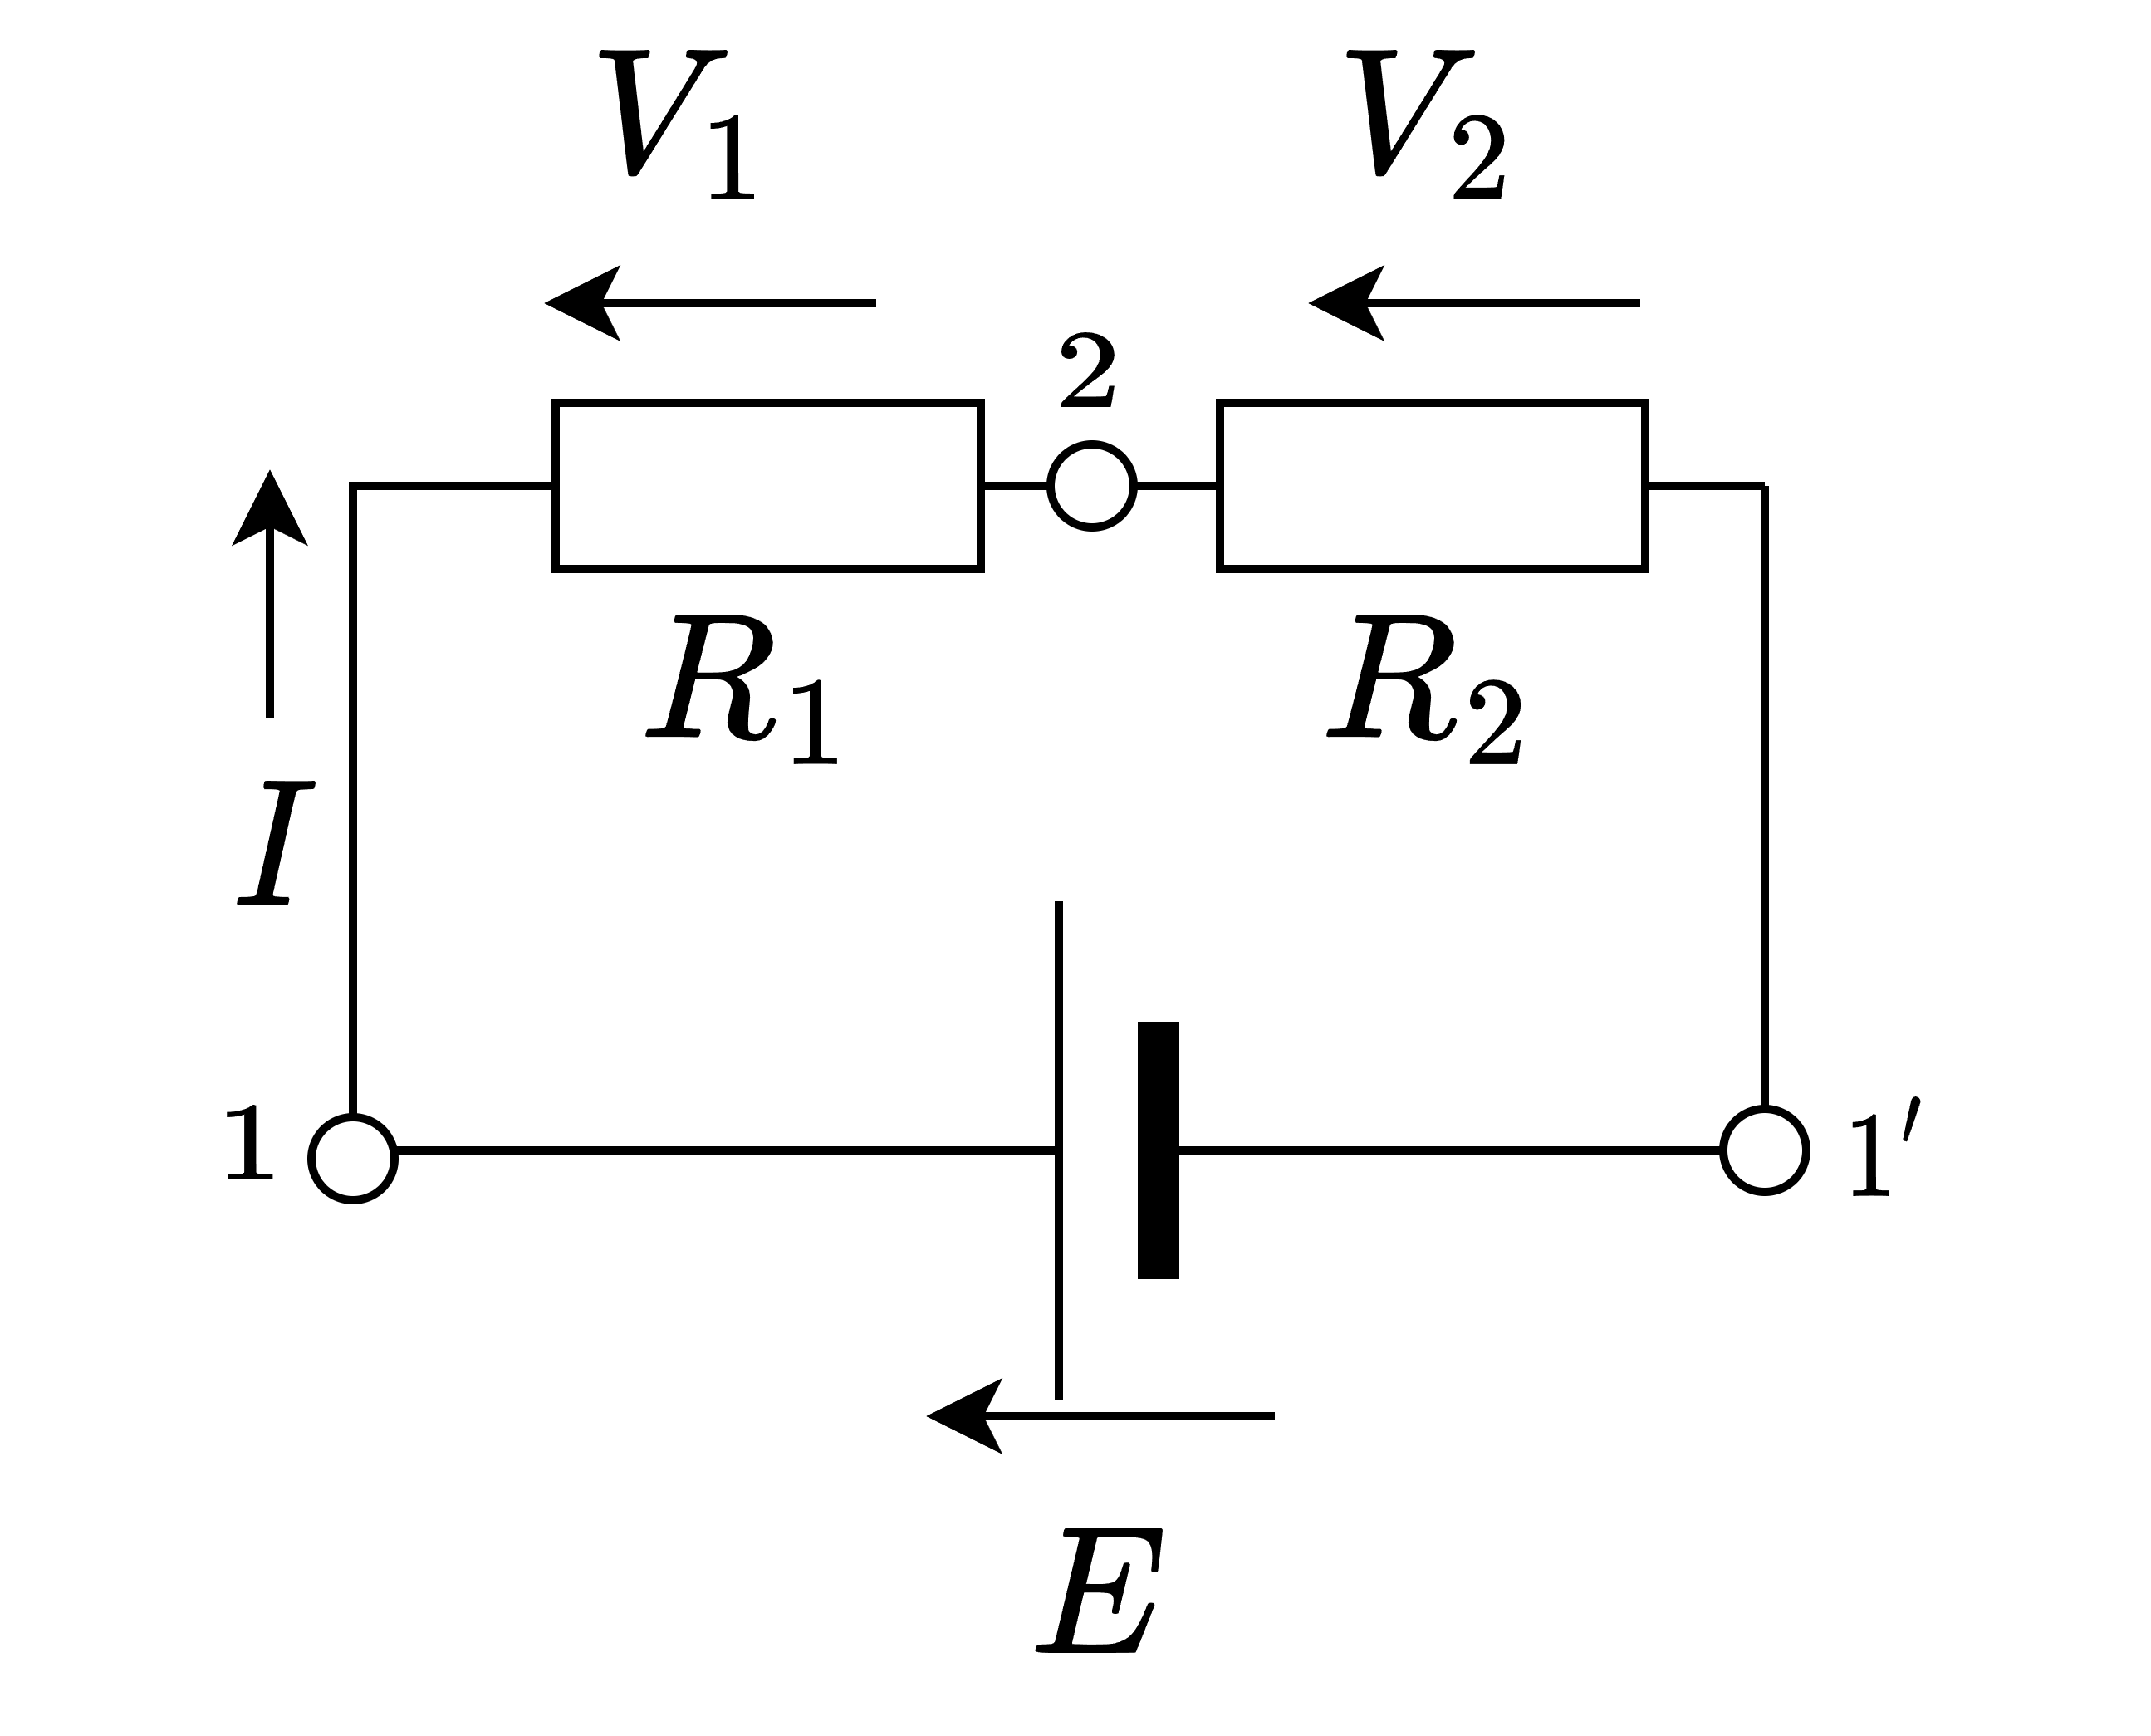
\includegraphics[keepaspectratio, scale=0.07]
       {img/ohm2.drawio.png}
  \caption{}
  \label{fig:voltup_down}
 \end{figure}


\subsection{キルヒホッフの法則}
オームの法則により、ループが1つしかない回路については解くことができる。
より一般的に、ループが複数の回路でも適用できる法則がキルヒホッフの法則である。



\subsubsection{キルヒホッフの電圧則(KVL)}
回路中にある閉ループをとる。
どのような経路を通ってきてもループを1周して戻ってきたときの電位は最初と同じである。

つまり、より複雑な回路についても、任意にループを定めたとき、
先に述べた式
\[
  (電圧上昇の和)-(電圧降下の和) =0
\]
が成り立つ。

一般にループ内に$n$個の電圧上昇があって$i$番目の電圧上昇が$E_i$と表され、$m$個の電圧降下があって$j$番目の電圧降下が$V_j$と表されるとき、以下の式が成り立つ。
\begin{equation}
  \sum_{i=1}^{n} E_i - \sum_{j=1}^{m} V_j = 0
\end{equation}



\subsubsection{キルヒホッフの電流則(KCL)}
ある点で回路が分岐しているとき、その点に流入する電流の総和とその点から流出する電流の総和は等しい。
つまり、分岐点に電荷が蓄積されることはない。

これを式に表そう。ある分岐点に$n$個の分岐があり、$i$番目の線に流れる電流を$I_i$とする。ただし、流入する方向を電流の正方向とする。このとき、次の式が成り立つ。

\begin{equation}
  \sum_{i=1}^{n} I_i = 0
\end{equation}





\subsection{閉路解析法}
キルヒホッフの法則を使えば理論的にはどのような回路を解くこともできる。
しかし、どの部分の値(電圧、電流)を仮定して、どのような立式をすればうまく解けるのかということは述べられていない。
ここでは、統一的な手順で回路を解くことができる方法のひとつとして、閉路解析法を紹介する\footnote{節点解析法というKCLをベースとした手法もあるが、閉路解析法の方がシンプルで使いやすいことが多い。本稿では節点解析法は省略する。}。
この方法はKVLを用いた方法であるから、電源がすべて電圧源である必要がある\footnote{後に紹介する電源の等価変換を用いれば電流源があっても解くことができる。}。

図\ref{fig:loop_analysis}のような回路を考えよう。この回路で各点に流れる電流はどのように表されるだろうか。
\begin{figure}[tbh]
  \centering
  
\includegraphics[keepaspectratio, scale=0.07]
       {img/loop.drawio.png}
  \caption{}
  \label{fig:loop_analysis}
 \end{figure}


この回路で、まず、2つの閉路に流れる電流(閉路電流、またはループ電流とよぶ)を仮定し、その2つの閉路に成り立つ方程式を導くと以下のようになる。

\begin{equation}
  \left\{ \,
      \begin{aligned}
      & E - R_1I_1 - R_2(I_1-I_2) = 0  \\
      & -R_2(I_2-I_1) - R_3I_2 = 0
      \end{aligned}
  \right.
  \end{equation}

これを解くことで、$I_1 = \dfrac{R_2+R_3}{R_1R_2 + R_2R_3 + R_3R_1}E$, 
$I_2 = \dfrac{R_2}{R_1R_2 + R_2R_3 + R_3R_1}$を得る。

一般的な回路において、仮定が必要な閉路電流の数$l$はグラフ理論の結果を用いることでわかる。
電気回路を節と辺で構成されたグラフと同一視する\footnote{何を節と辺に取るかというのは色々なやり方があるようで、たとえば、素子を節に取るやり方や、配線の交わる点を節に取るやり方がある。個人的には後者の方がわかりやすいと思う。配線の交わる点とはある点から3つ以上の分岐があるものを指しているが、仮に2つしか分岐がない点(つまり配線の交点ではない点)を節にとっても、その分辺の数も増えるため結果は変わらない。}と、$l$は節の数をn、辺の数をbとすれば、以下の式が成り立つ。
\[
  l = b-n+1
\]

\subsection{キルヒホッフの法則の問題点}
キルヒホッフの法則は理論的には万能であり、十分な情報が与えられていればすべての回路を連立方程式に帰着させて解くことができる。

しかし、手計算で回路を解く場合、計算ミスをしやすいうえ、最善手とはならず、もっと楽に解く方法がある場合も多い。
なぜなら、キルヒホッフの法則では一般的に、仮定したすべての未知数を求めるまで解が定まらない。
実際に回路を解きたいときは、ある部分のみを知りたい場合も多いから遠回りになってしまうのである。

ここからは、様々な解析手法を学び、キルヒホッフの法則から卒業しよう。
\subsection{分圧、分流}
\subsubsection{分圧}
キルヒホッフの方法から直ちに求められる公式が分圧、分流の式である。
いま、再び\ref{fig:volt_partial}に示す直列回路を考えよう。
この回路についてキルヒホッフの法則を用いて解析すれば、以下の式が成り立つことが直ちにわかる。
これを用いれば単純な直列回路ではキルヒホッフの法則を用いる必要がなくなるので時間短縮に役立つ。
\begin{align}
  V_1 &= \frac{R_1}{R_1+R_2}E\\
  V_2 &= \frac{R_2}{R_1+R_2}E
\end{align}


\begin{figure}[tb]
  \centering
  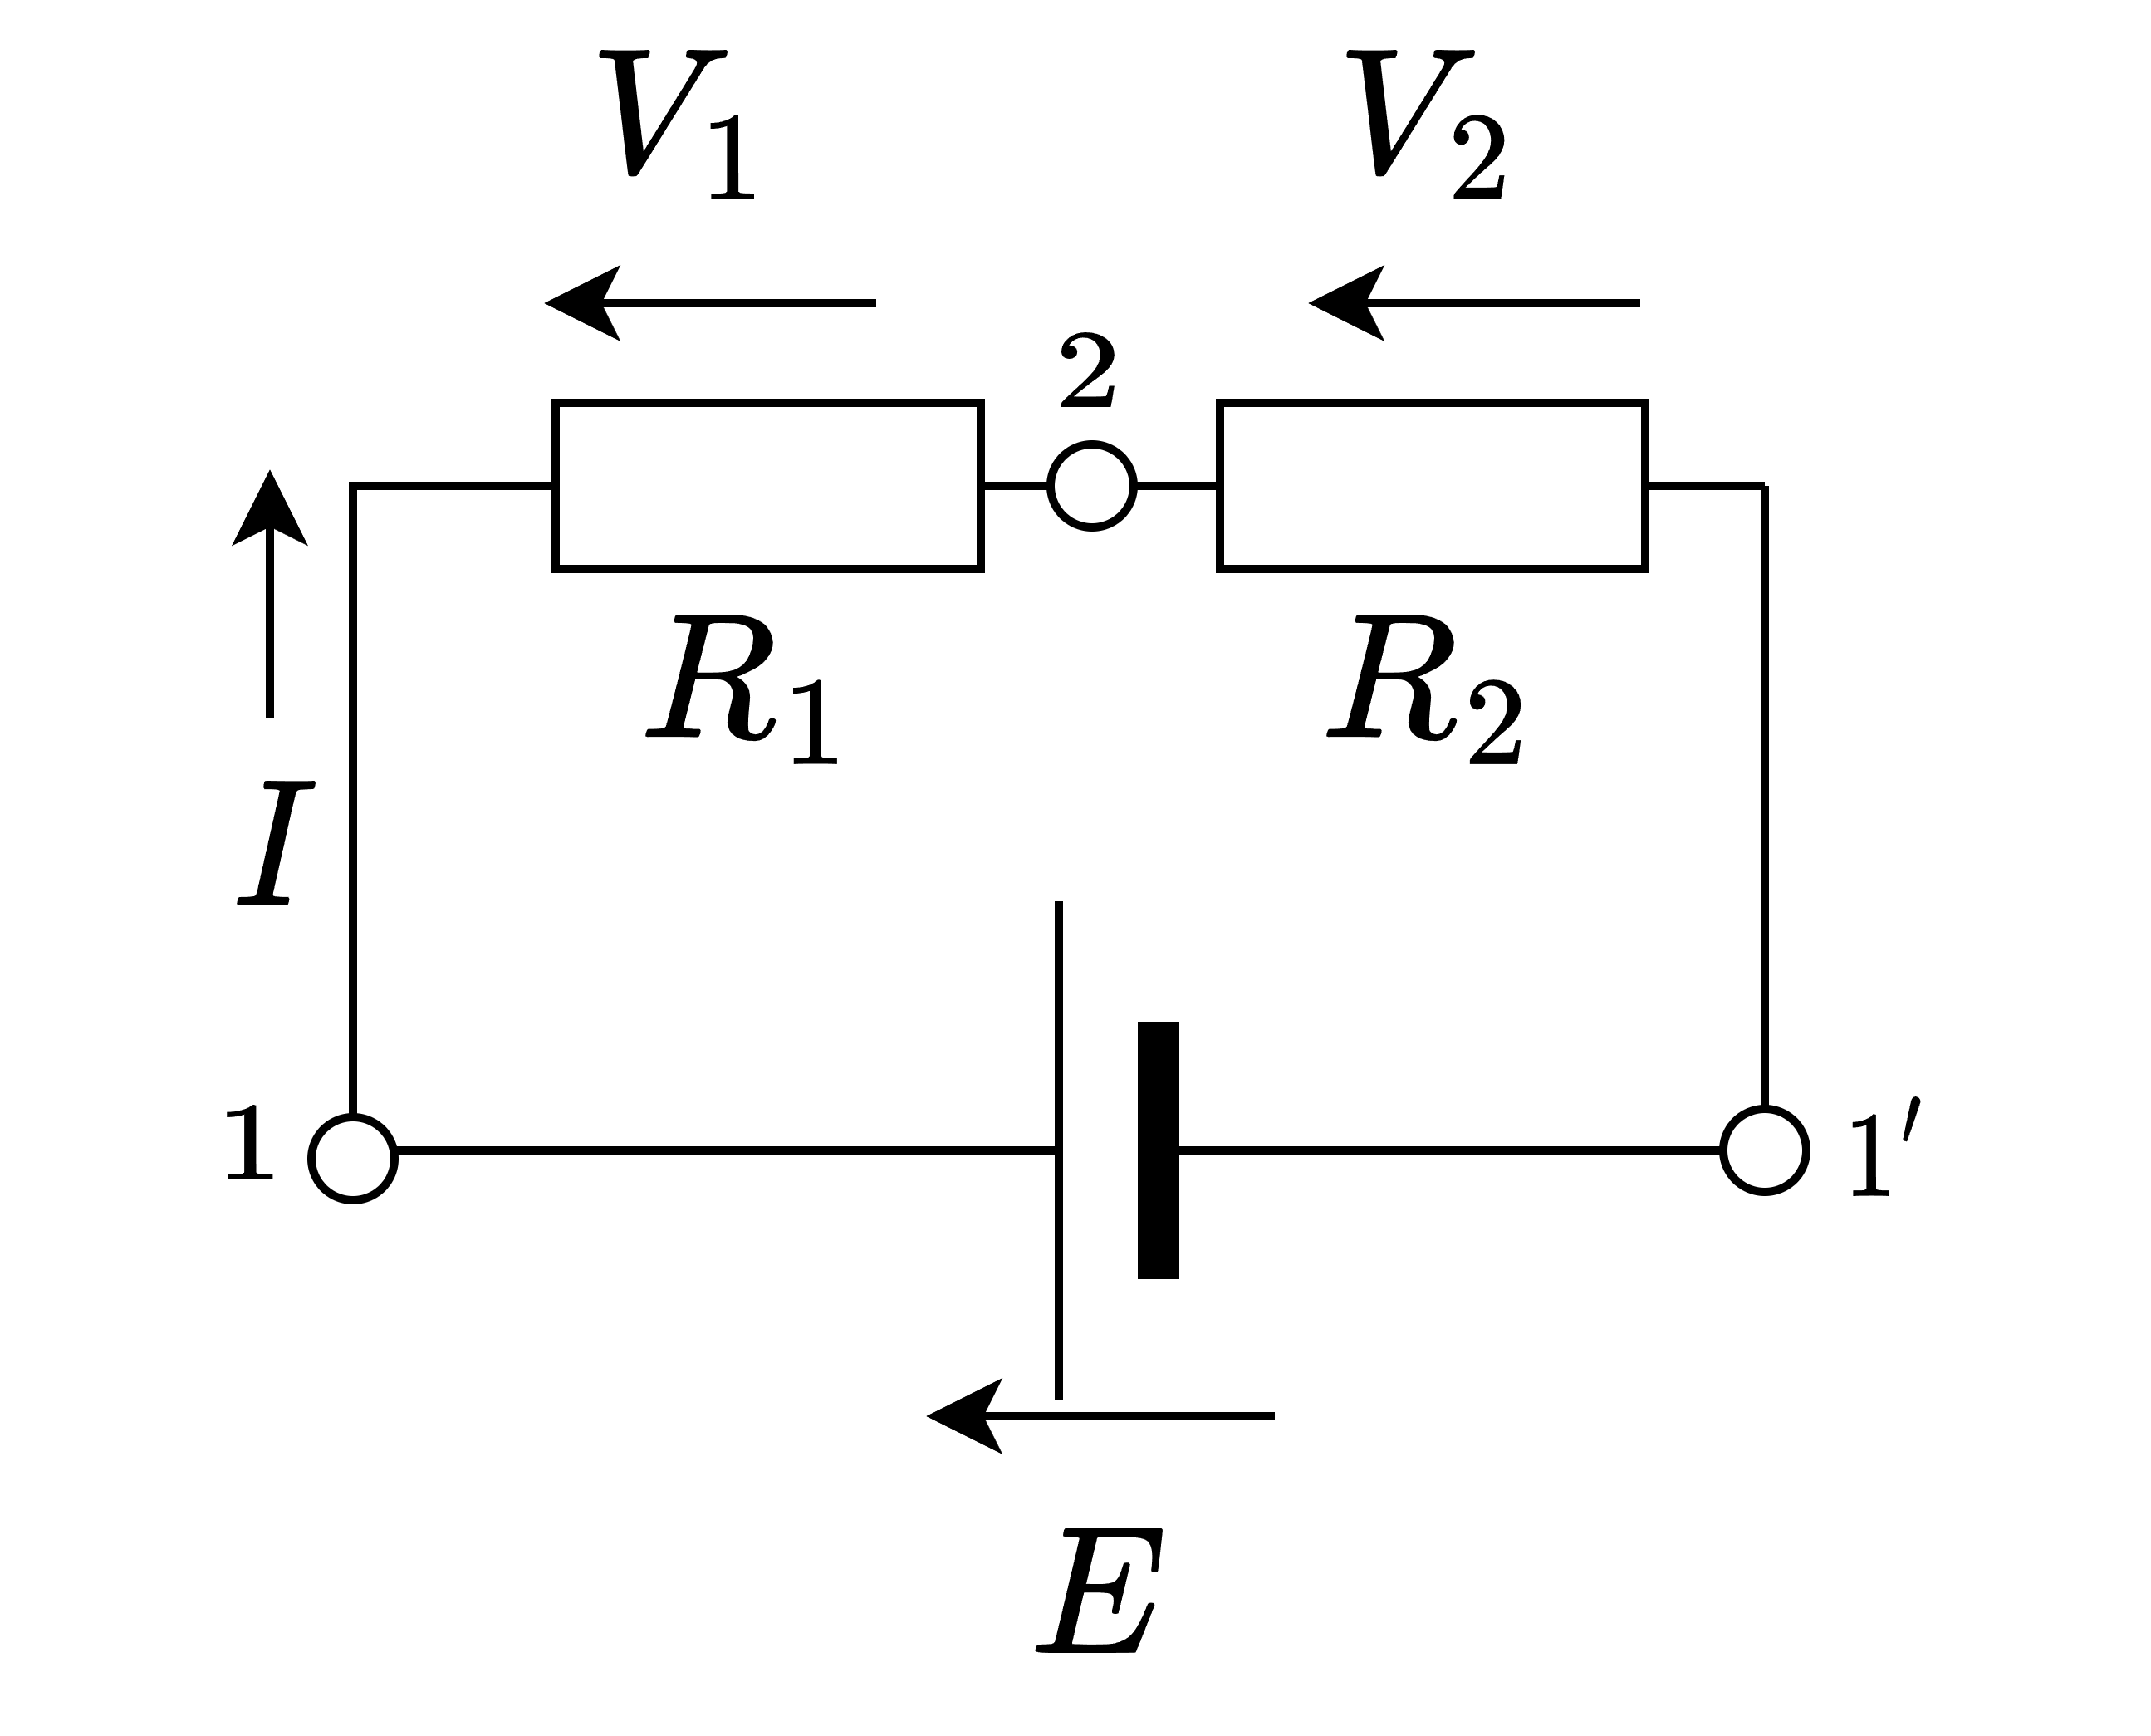
\includegraphics[keepaspectratio, scale=0.07]
       {img/ohm2.drawio.png}
  \caption{}
  \label{fig:volt_partial}
 \end{figure}

\subsubsection{分流}
次に、図\ref{fig:current_partial}の並列回路を考えよう。
この回路では$E$から全体に電流$I$が流れていて、分岐点で$R_1$側に$I_1$、$R_2$側に$I_2$が流れている。
これらの電流の関係を考えると、以下の式が成り立つ。
\begin{align}
  I_1 &= \frac{R_2}{R_1+R_2}I\\
  I_2 &= \frac{R_1}{R_1+R_2}I
\end{align}
分圧の式と比べると、分子の抵抗が逆になっていることがわかる。
これらの式は形が似ているので覚えにくいかもしれない。
そういうときには片方の抵抗を$0$や$\infty$ であると考えてみると正しい式かどうか確認することができる。

\begin{figure}[tb]
  \centering
  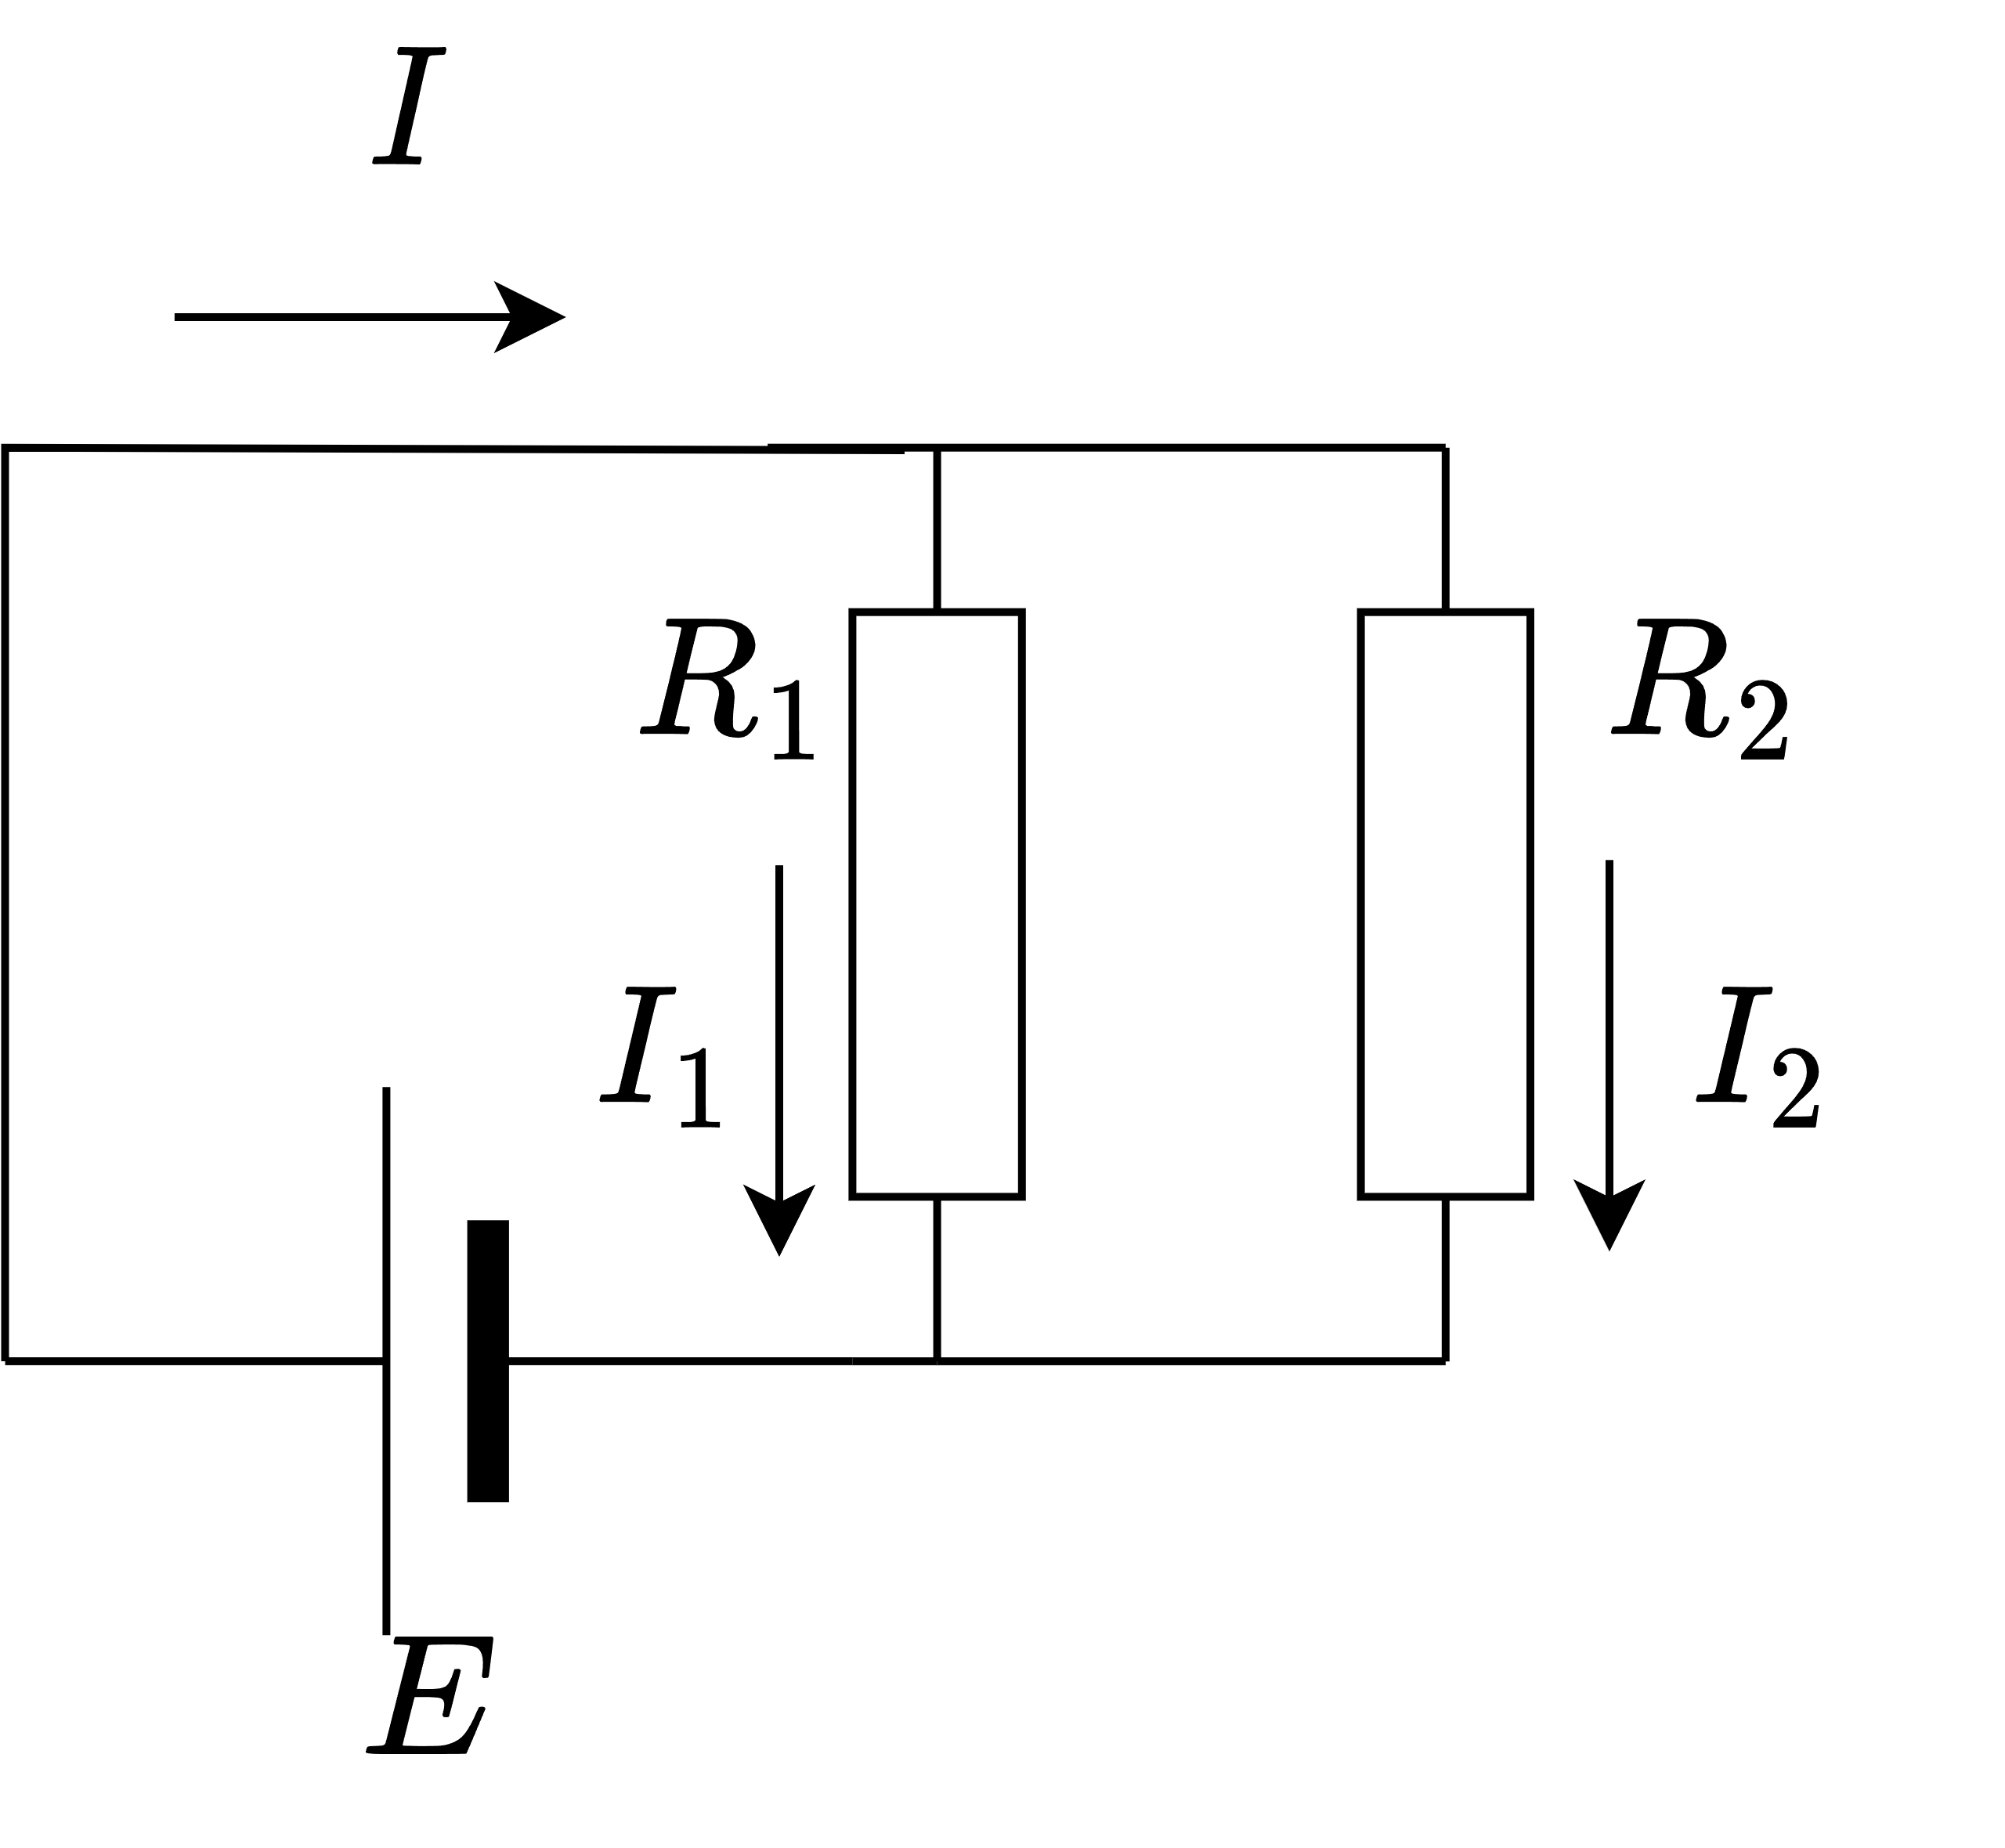
\includegraphics[keepaspectratio, scale=0.07]
       {img/para.drawio.png}
  \caption{}
  \label{fig:current_partial}
 \end{figure}

\subsection{合成抵抗}
複数の抵抗が直列や並列に配置されており、個々の抵抗に流れる電流や電圧には興味がないが、全体で流れている電流を求めたいということがあるだろう。あるいは、分流を求めるために先に全体の電流を求めたいことがあるかもしれない。
そういった際には、回路に接続された複数の抵抗をまとめて1つの合成抵抗とみなして解析する必要がある。

直列回路から始めよう。図\ref{fig:volt_partial}の回路において、
2つの直列抵抗をまとめてひとつの合成抵抗Rとすると、オームの法則より、
\[
  E = RI
\]
また、式\eqref{eq:ohm2}より、
\[
  E = (R_1+R_2)I
\]
これらの2式を比較すると、
\[
  R=R_1+R_2
\]
である。直列に接続された合成抵抗は単純に和を取れば良い。

次に、並列回路について考えよう。
図\ref{fig:current_partial}において、次の3式が成り立つ。
\begin{align}
  E &= R_1I_1\\
  E &= R_2I_2\\
  I &= I_1 + I_2
\end{align}

これら3式から、 $I = (\frac{1}{R_1} + \frac{1}{R_2}) E$が導かれ、これを合成抵抗Rを用いたオームの法則と比較すると、
\begin{align}
  \frac{1}{R} = \frac{1}{R_1} + \frac{1}{R_2}
\end{align}
よって、
\begin{equation}
  R = \frac{R_1R_2}{R_1+R_2}
\end{equation}
が成り立つ。

ここで、並列回路の合成抵抗をコンダクタンスG=1/Rを用いた式で表すと、以下のようになる。
\[
  G = G_1 + G_2
\]
直列回路では抵抗を用いた式が簡単に表されるが、並列回路ではコンダクタンスを用いると簡単に計算できる場合がある。
\subsection{電源の等価変換}
\ref{sec:source}節で電源には2種類あることを説明した。
これらは互いに相容れないものであるわけではなく、相互に変換することができる。
改めて電源の図\ref{fig:equvalent_source}を示す。
図の左の電圧源を右の電流源に変換するときには、以下のようにおけば良い。
\begin{align}
  I &= \frac{E}{R_1}\\
  R_2 &= R_1
\end{align}

逆に、電流源を電圧源の形に変換するときには以下のようにおけばよい。
\begin{align}
  E &= IR_2\\
  R_1 &= R_2
\end{align}

これらの証明は\ref{sec:Thevenin}節で紹介するテブナンの定理を用いると簡単に与えられる。
\begin{figure}[tb]
  \centering
  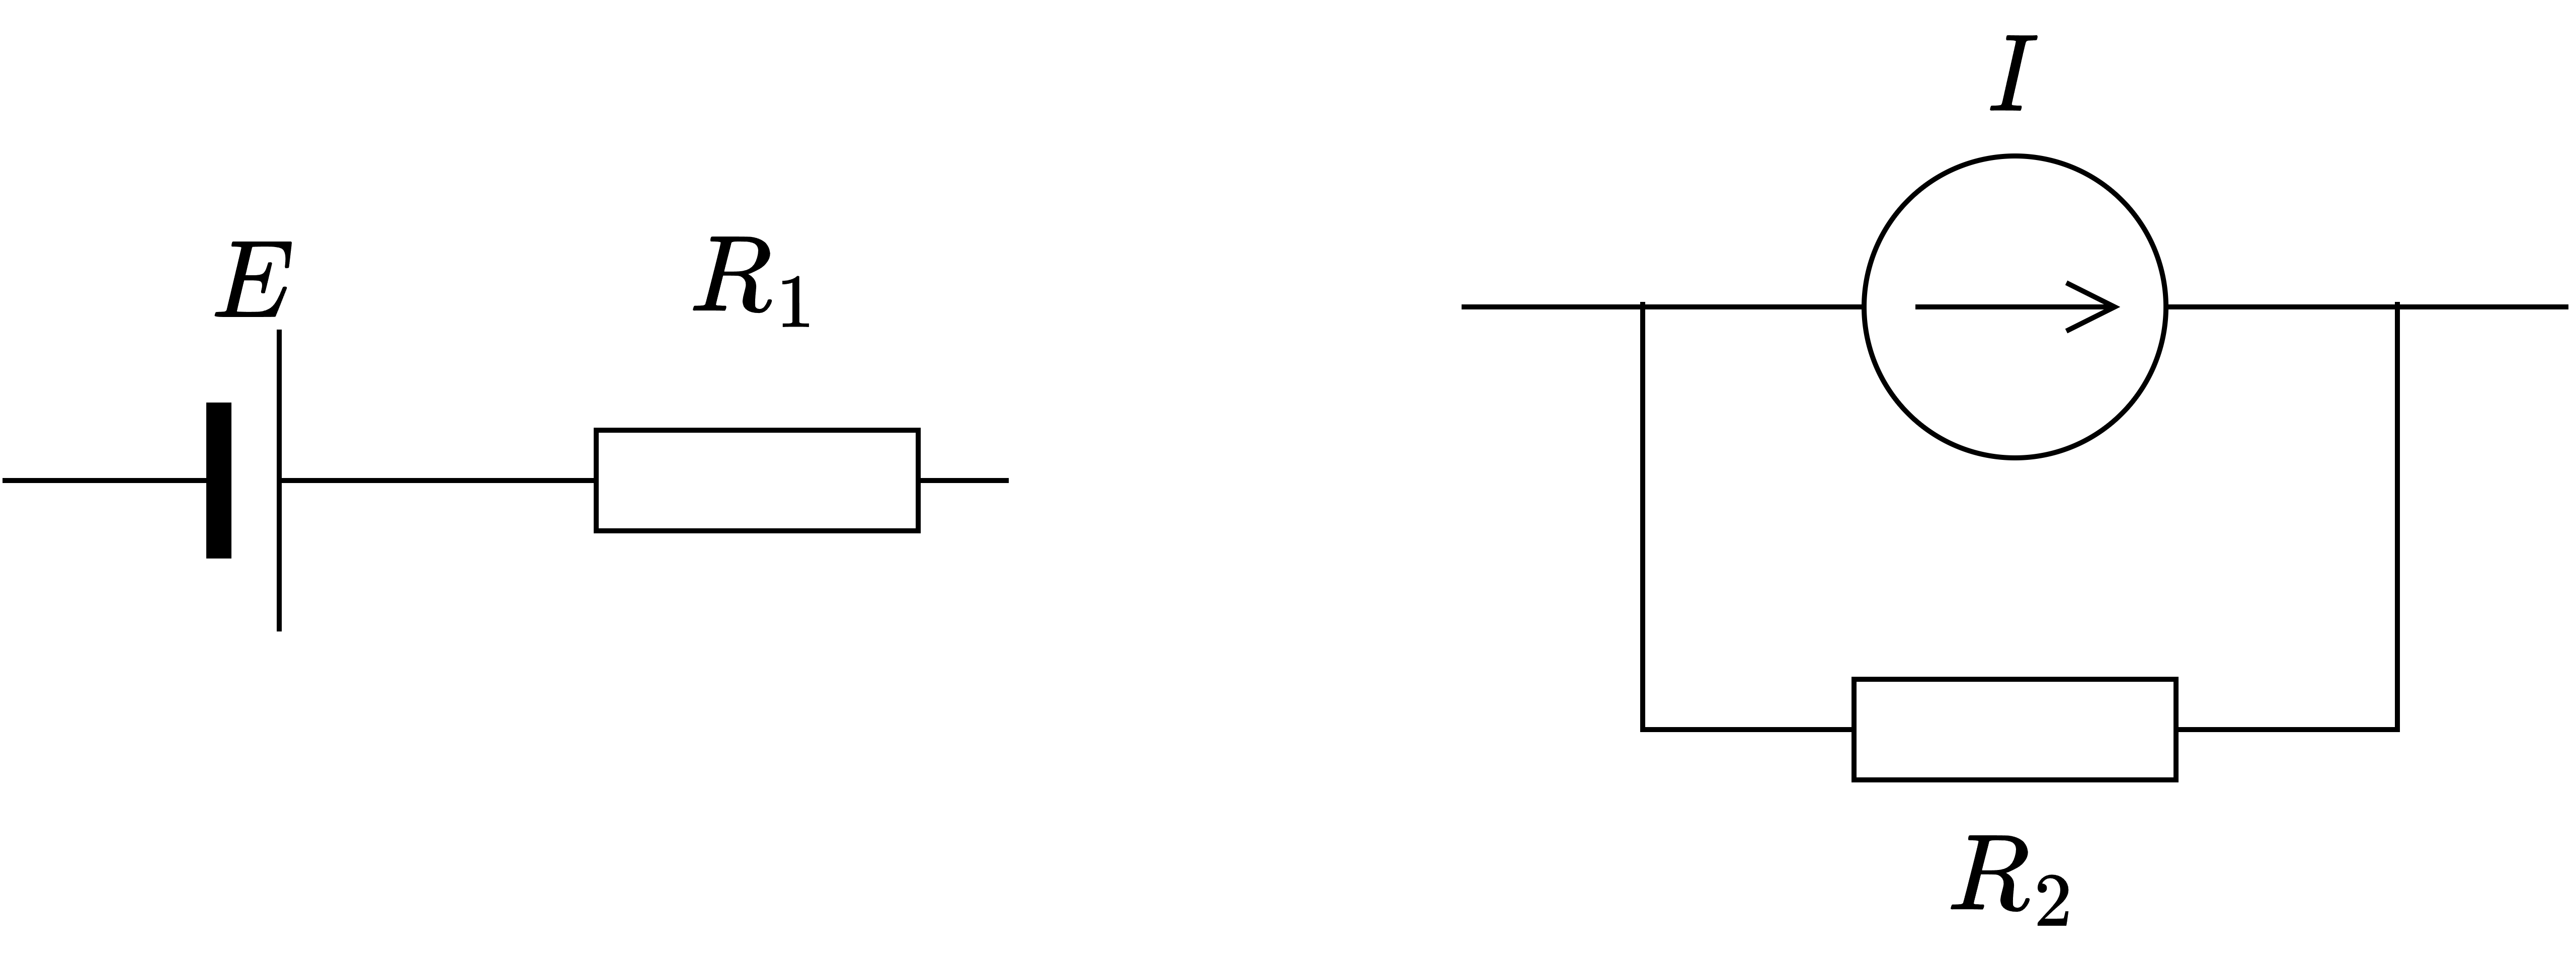
\includegraphics[keepaspectratio, scale=0.07]
       {img/real_battery2.drawio.png}
  \caption{現実の電源の等価電圧源と等価電流源}
  \label{fig:equvalent_source}
 \end{figure}

この変換規則を見たとき、実際の回路には複数の抵抗があるが、どこまでを内部抵抗として扱えば良いのか疑問をもつ人がいるかもしれない。結論から言うとそれは自由であり、どこまでの抵抗を内部抵抗として扱っても問題ない。
後に説明するが、この変換規則と合成抵抗の公式を繰り返し利用して回路を簡単な等価回路に置き換えて解くことができる。

\subsection{重ね合わせの理}
重ね合わせの理は、複数の電源が回路中に存在するとき、任意の地点の電流および、電圧はある1つの電源のみ機能していて他の電源を`ゼロ'にしたときの値をすべての電源について重ね合わせたものに等しい、という原理である。この原理は回路に線形性があるときのみ成り立つ。
電源をゼロにするとは、電圧源の電圧を0、電流源のある枝の電流を0にするということである。
つまり、図\ref{fig:short_open}のように、電圧源を短絡(ただの配線に置き換える)、電流源を開放する(配線を切り離す)ということに相当する。

\begin{figure}[tbh]
  \centering
  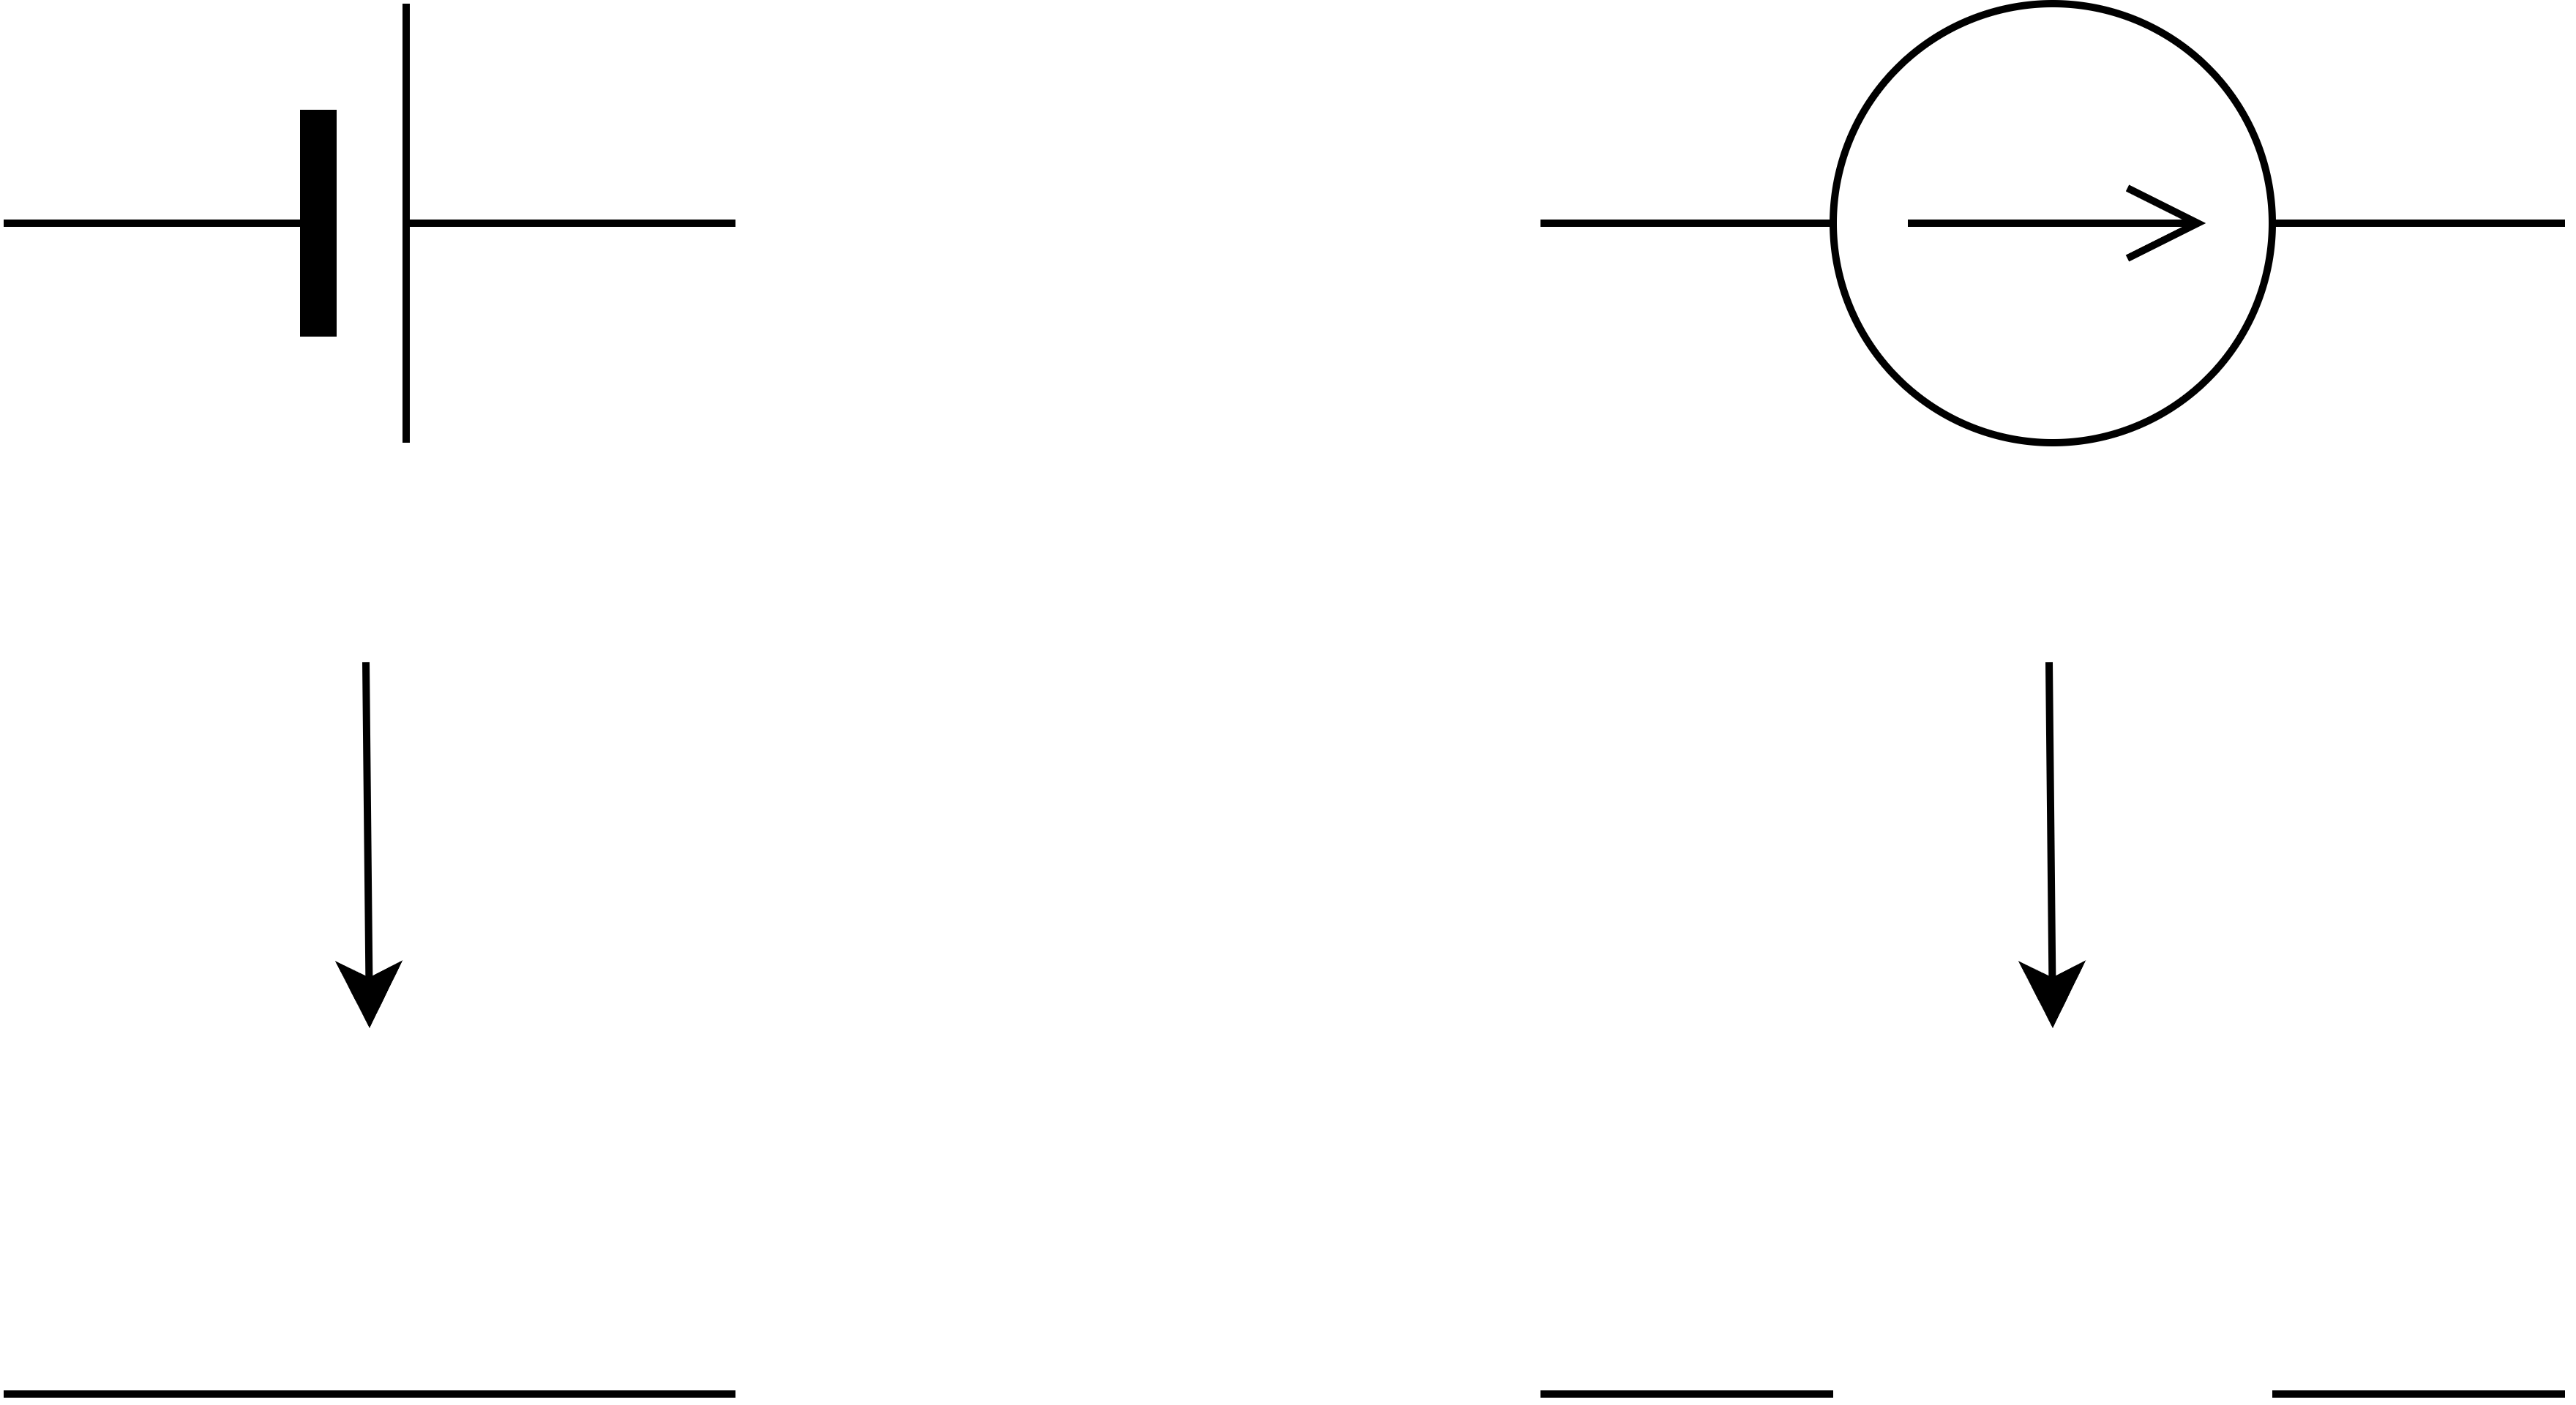
\includegraphics[keepaspectratio, scale=0.07]
       {img/short_open.drawio.png}
  \caption{電圧源の短絡(左)と電流源の開放(右)}
  \label{fig:short_open}
 \end{figure}


たとえば、2つの電源として電圧源$E_0$と電流源$I_0$が存在する回路があり、ある点$P$での電流$I$が知りたいとしよう。
まず、$E_0$の働きを知るために、$E_0$のみ機能をもたせた状態にし、$I_0$の両端を開放する。
その状態での$P$での電流を求めると$I_1$であった、とする。

次に$I_0$の働きを知るために、$I_0$のみ機能をもたせた状態にし、$E_0$の両端を短絡する。
その状態での$P$での電流を求めると$I_2$であった、とする。

これらの結果から、$I=I_0+I_1$が求められる。

電源が複数あったからといってキルヒホッフの法則が使えなくなるわけではない。
重ね合わせの原理は、より複雑な回路を解析するときに有用である。



\subsection{テブナンの定理}\label{sec:Thevenin}
テブナンの定理は、複数の素子から構成された回路網から取り出した2つの端子間を図\ref{fig:Thevenin}のように非常に単純な等価回路に置き換える定理である。この図における等価回路の電圧$E$を(2端子間を開放したときの電圧であるから)開放電圧と呼ぶ。$R_0$は2つの端子から内部を見込んだ内部抵抗である。
2つの端子間に抵抗$R$が接続されているとき、この抵抗を流れる電流$I$は以下のように表される。
\[
  I = \frac{1}{R_0+R}E
\]
この定理を実際に適用する回路において、考える端子間は必ずしも開放されている必要はない。定理を適用するときのみ自分で開放して考えれば良い。
内部抵抗を求めるときには、回路網側の電源について、電圧源は短絡、電流源は開放して考える。

\begin{figure}[tbh]
  \centering
  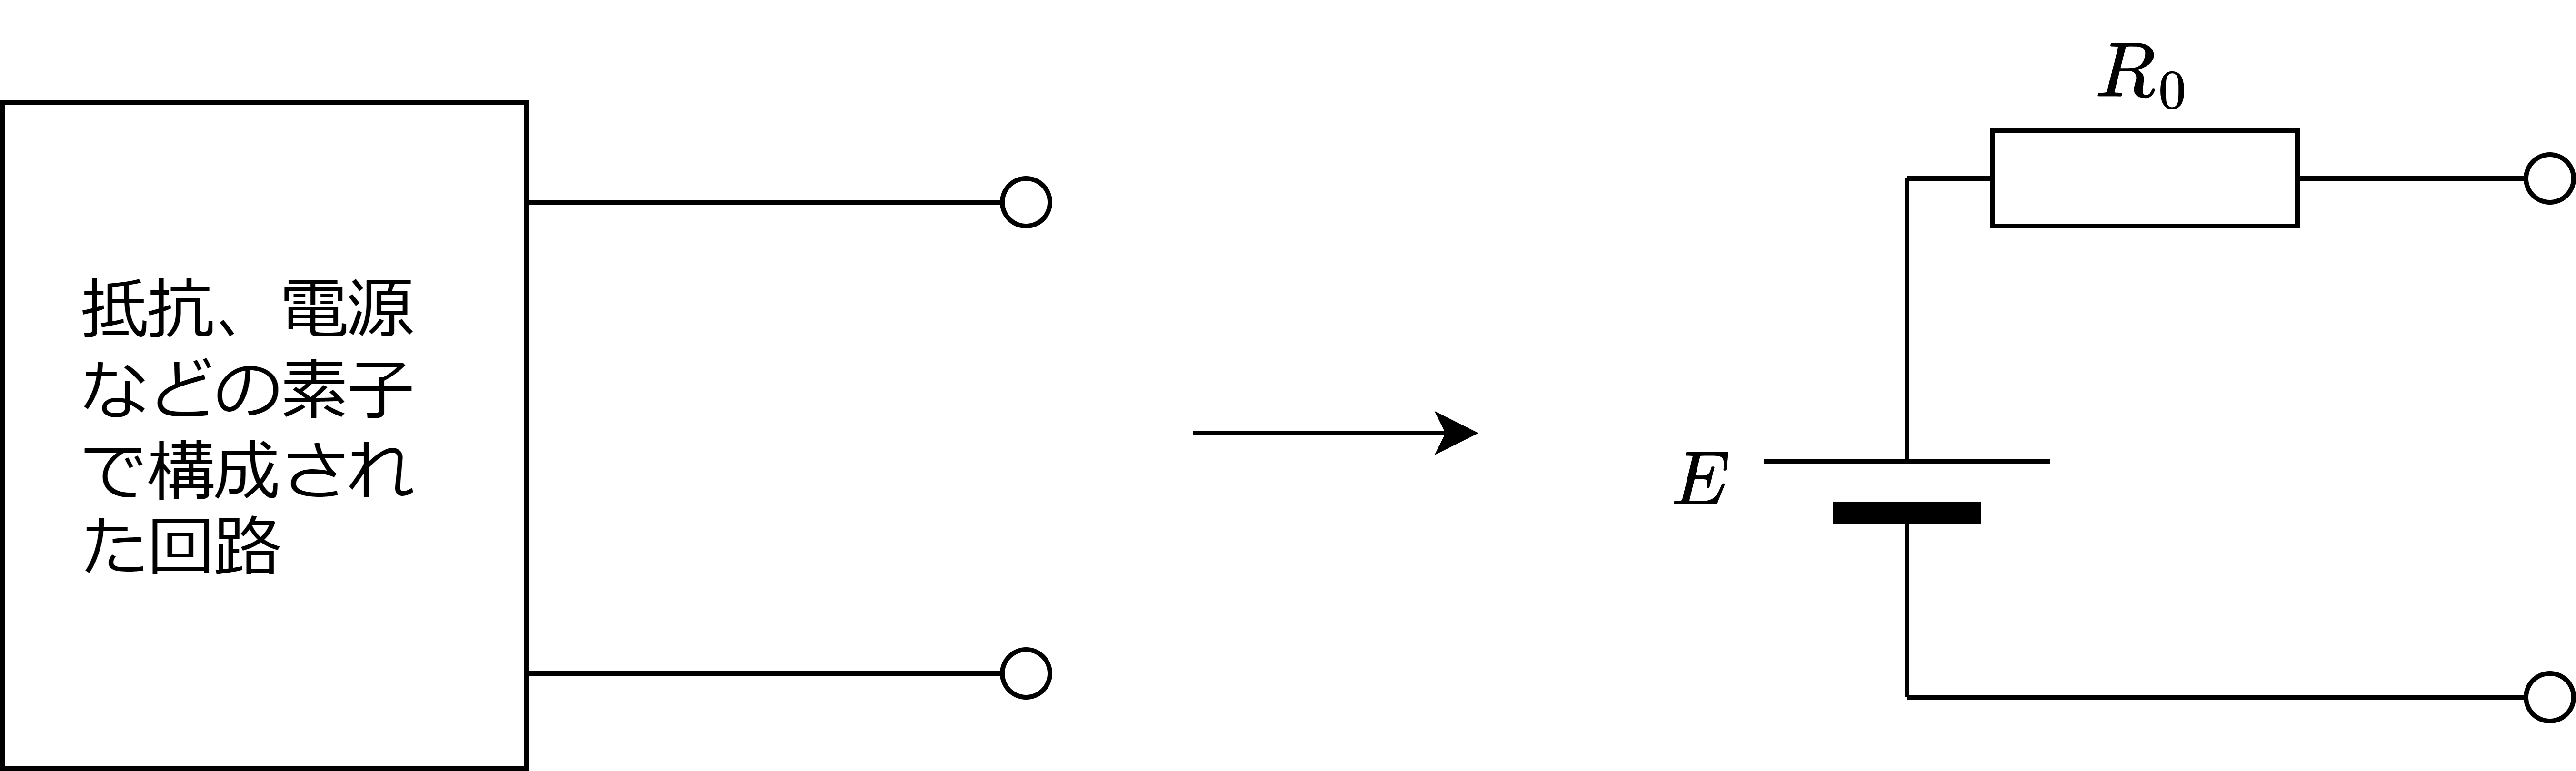
\includegraphics[keepaspectratio, scale=0.07]
       {img/Thevenin.drawio.png}
  \caption{テブナンの定理}
  \label{fig:Thevenin}
 \end{figure}



\subsection{定理の利用例}

定理を活用して、以前閉路解析法で解いた回路を改めて解いてみよう。

\begin{itembox}[l]{問題}
図\ref{fig:loop_re}の回路において、$I_1$と$I_2$を求めよ。
\begin{figure}[H]
  \centering
  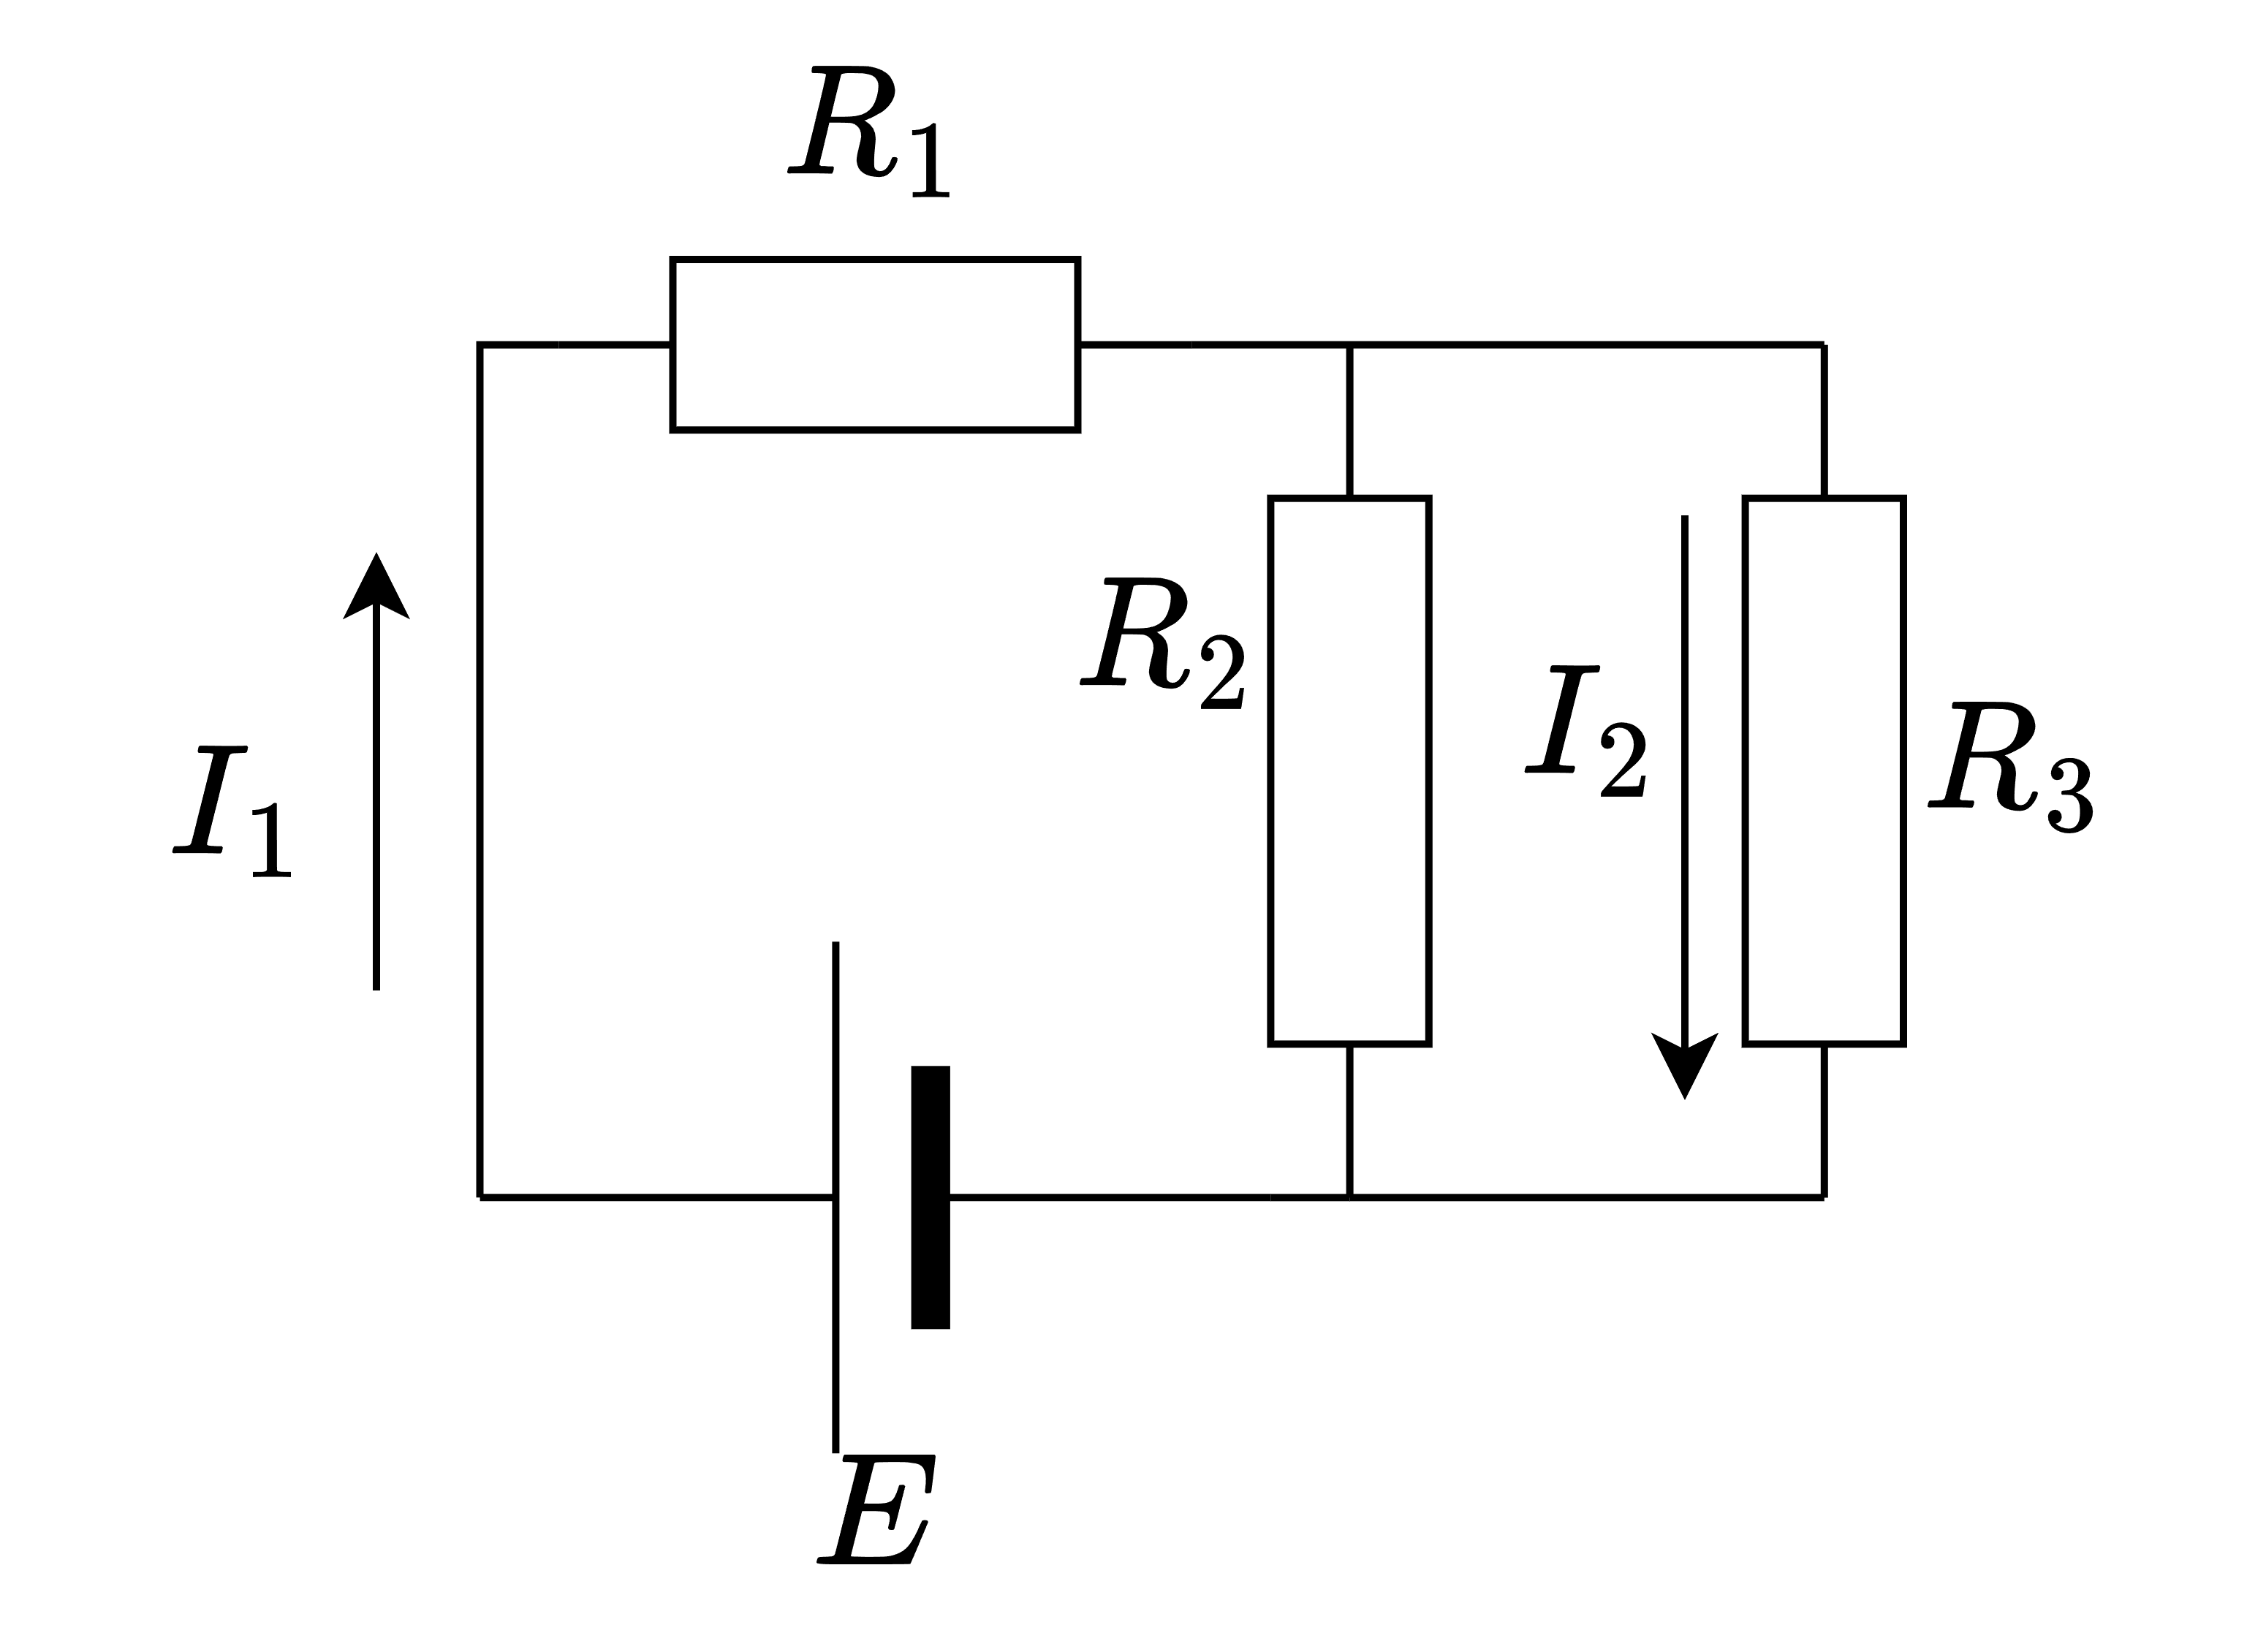
\includegraphics[keepaspectratio, scale=0.07]
       {img/loop_re.drawio.png}
  \caption{}
  \label{fig:loop_re}
 \end{figure}

\end{itembox}

\subsubsection{分流と合成抵抗による解法}
並列の抵抗を\paral の記号で表すとする。
全体の合成抵抗は $R_1+R_2\paral R_3 = R_1+\para{R_2}{R_3} = \frac{R_1R_2+R_2R_3+R_3R_1}{R_2+R_3}$であるから、オームの法則より
\[
  I_1 = \frac{R_2+R_3}{R_1R_2+R_2R_3+R_3R_1}E
\]

次に、分流を用いれば、

\begin{align}
  I_2 &= \frac{R_2}{R_2+R_3} I_1\\
  &= \frac{R_2}{R_1R_2+R_2R_3+R_3R_1}E \quad .
\end{align}



\subsubsection{電源の等価変換による解法}
$I_1$は工夫できないので省略する。

$I_2$を求めよう。
図\ref{fig:loop_eqv}のように、電源の変換と合成を繰り返し適用すれば、最終的にオームの法則が適用できる形になり、
\[
  I_2 = \frac{1}{R_1 \paral R_2 + R_3} \frac{R_2}{R_1+R_2}E
\]
よって、
\[
  I_2 = \frac{R_2}{R_1R_2+R_2R_3+R_3R_1}E \quad .
  \]

\begin{figure}[bth]
  \centering
  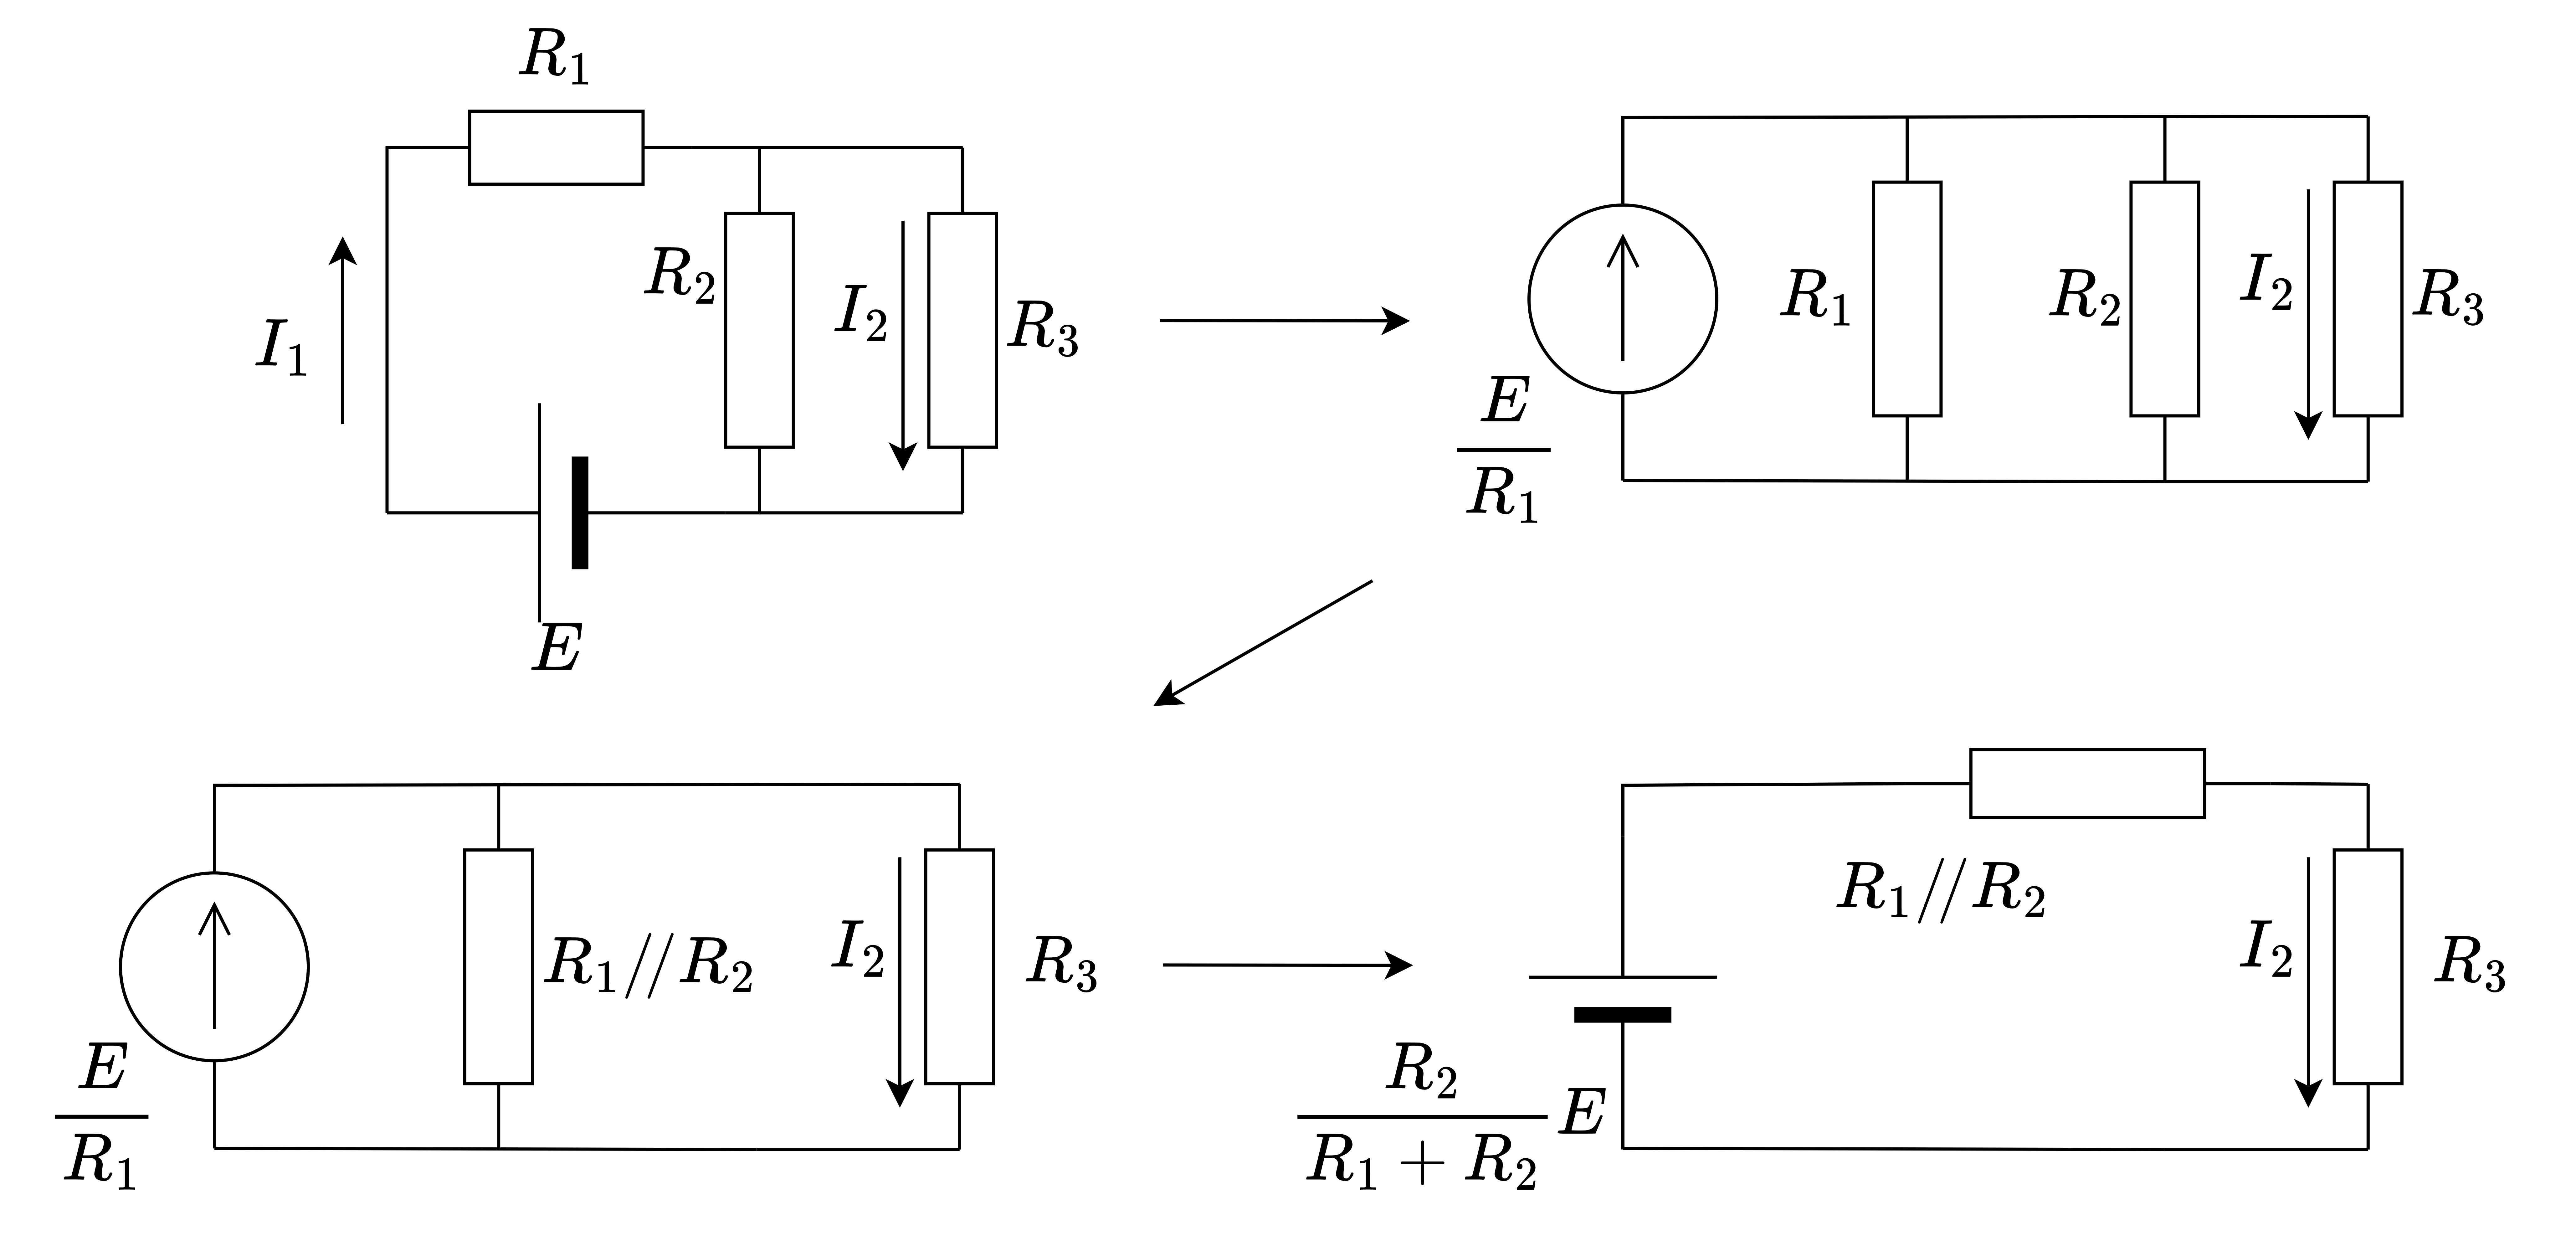
\includegraphics[keepaspectratio, scale=0.05]
       {img/loop_eqv.drawio.png}
  \caption{電源の等価変換と抵抗の合成を繰り返す過程}
  \label{fig:loop_eqv}
 \end{figure}

先にも述べたが、この方法は段階的にテブナンの定理を利用しているのと等価である。

\subsection{テブナンの定理による解法}
$I_1$については、$R_1$の両端を開放して開放電圧と内部抵抗を考えると先に示した分流と合成抵抗による解法と全く同じ形になるため省略する。

$I_2$について、$R_3$の両端を開放して、開放電圧と内部抵抗を求めよう。
開放電圧$V$は、$R_2$の両端の電圧に等しい。よって、分圧を用いて
\[
  V = \frac{R_2}{R_1+R_2}E
  \]

内部抵抗は、$E$を短絡して考えると、
\begin{align}
  R &= R_1 \paral R_2\\
    &= \para{R_1}{R_2}
\end{align}

よって、$R_3$に流れる電流は、

\begin{align}
  I &= \frac{1}{R+R_3}V\\
    &= \frac{R_2}{R_1R_2+R_2R_3+R_3R_1}E \quad .
\end{align}


このように種々の公式を利用することにより、キルヒホッフの法則よりも楽に答えを求めることができる。











\section{正弦波交流回路の解析}

\subsection{正弦波交流}
\[
  v(t) = V_m \sin(\omega t + \theta)
\]
の形で表された電圧(または電流)を持つ回路を正弦波交流回路という。

\omega を角周波数といい、周波数$f$を用いて$\omega = 2 \pi f$と表される。
$V_m$を振幅、
\theta を位相といい、交流回路においては、振幅のほかに位相のズレまで考慮する必要が出てくる。
$\theta = 0$のときに対し、たとえば$\theta = -\frac{\pi}{2}$のときを位相が$\frac{\pi}{2}$遅れているなどと言い、
逆に$\theta >0 $であれば位相が進んでいると言う。

\subsection{交流回路上の素子}

\subsubsection{抵抗}
交流回路上に抵抗がある場合について考察しよう。
直流回路におけるオームの法則はRが不変ならば$E=RI$が成り立つことを約束するものであった。
実はこの法則は、電圧や電流がが時間変化したとしても成り立つとして拡張してよい。
ゆえに、抵抗の両端に正弦波の電圧を印加すれば、
\begin{align}
  v(t) &= Ri(t)\\
  i(t) &= \frac{V_m}{R} \sin(\omega t + \theta)
\end{align}

よって位相は同相であり、電圧の振幅$V_m$、電流の振幅$I_m$に対し、
\[
  V_m = R I_m
\]
の関係がある。

\subsubsection{キャパシタ}
キャパシタ、またはコンデンサは、2つの導体板が向き合った構造の素子であり、両端に電圧$V$を印加すると、電荷移動が発生して2つの導体板がそれぞれ$+Q$、$-Q$ [C] に帯電する。このとき各導体板に蓄えられる電荷量は与えた電圧に比例し、
\[
  Q = CV
  \]
の関係をみたす。この定数$C$を静電容量、または単に容量といい、単位をファラッド [F] で表す。

電流の基本定義から、$i(t) = \dft{q(t)}$であるから、この$q$に$q(t)=Cv(t)$を代入すれば、
\[
  i(t) = C \dft{v(t)} \quad .
\]
この関係は逆に積分形式でも表され、
\[
  v(t) = \frac{1}{C}\int_{-\infty}^{t} i(t) \diff t \quad .
\]
キャパシタ$C$の両端に正弦波電圧を印加すれば、
\begin{align}
  v(t) &= V_m \sin \omega t\\
  i(t) &= \omega CV_m \sin (\omega t + \ang{90})
\end{align}
となるから、
電流の位相が電圧より常に\ang{90}進み、電圧の振幅$V_m$、電流の振幅$I_m$に対し、
\[
  V_m = \frac{1}{\omega C} I_m
\]
が成り立つ。$\frac{1}{\omega C}$を容量性リアクタンスという。



\subsubsection{インダクタ}
インダクタはコイルとも呼ばれる、鉄心、フェライトコアまたは空心にエナメル線等の導線を巻き付けた素子である。
電磁気学によれば、コイルに流れた電流が時間変化すると、自己誘導により逆起電力$v(t)$が$i(t)$と逆向きに発生し\footnote{電磁気学においては、電流に沿った向きに$v = -L\dft{i}$と、符号付きで与えられるが、はじめから電流と逆向きを正方向にとっておけばマイナスを付ける必要はない。}、以下のように表される。


\begin{equation}
  v(t) = L \dft{i(t)}
\end{equation}

この関係は以下の積分形式でも表される。

\begin{equation}
  i(t) = \frac{1}{L}\int_{-\infty}^{t} v(t)\diff t
\end{equation}

これらの式において、$L$をインダクタンスと呼び、ヘンリー [H]の単位を用いる。

インダクタ$L$の両端に正弦波電圧を印加すれば、


\begin{align}
  v(t) &= V_m \sin \omega t\\
  i(t) &= \frac{1}{\omega L} V_m \sin(\omega t - \ang{90})
\end{align}
となるから、
電圧の位相は電流の位相よりも常に\ang{90}進んでおり、電圧の振幅$V_m$、電流の振幅$I_m$に対し、
\[
  V_m = \omega L I_m
\]
の関係がある。$\omega L$を誘導性リアクタンスという。

\subsection{実効値}

\[
  V_e = \sqrt{\frac{1}{T}\int_{0}^{T} v^2(t) \diff t}
\]
のように2乗平均平方根値で定義される電圧値(または電流値)を実効値という。
ただし、$T$は周期である。正弦波交流に対しては、
\begin{align}
  V_e &= \frac{V_m}{\sqrt{2}}\\
  I_e &= \frac{I_m}{\sqrt{2}}
\end{align}
を満たす。
一般的に100 V の交流などというときには、実効値を示している。

\newcommand{\vsin}{V_m \sin\omega t}
\newcommand{\isin}{I_m \sin(\omega t + \theta)}
\subsection{交流回路の例}
\newcommand{\wL}{\omega L}
\newcommand{\wC}{\omega C}
\subsubsection{RL回路}
まず、正弦波交流電源$e(t) = \vsin$と抵抗$R$、インダクタ$L$を直列接続した回路を考えよう。
このとき回路方程式は、
\[
  Ri +L \dft{i} = \vsin
\]
このとき、回路が接続された瞬間は過渡現象が生じるが、十分長い時間が経つと応答電流も正弦波となり、そこから逸脱することはない。この状態を定常状態と呼ぶ。この章では定常状態のみを考えるものとする。
この式において、応答電流の一般解は微分方程式を解けば得られるが、定常状態の解のみを求めるならば、応答電流の形を$i(t) = \isin$とおいて解けば良い。
そのように解けば、
\[
  i(t) = \frac{V_m}{\sqrt{R^2 + \omega^2 L^2}} \sin (\omega t + \theta), \quad \theta = -\tan^{-1}(\frac{\omega L}{R})
\]
これを解く過程で三角関数の合成を用いた。

\subsubsection{RC回路}
同様に抵抗$R$と、キャパシタ$C$を直列接続した回路を考えよう。
このとき回路方程式は、キャパシタにかかる電圧を$v$とすれば
\begin{align}
  Ri + v &= \vsin \\
  i = C\dft{v}
\end{align}
同じように解を仮定して解けば
\[
  i(t) = \frac{\omega CV_m}{\sqrt{1+\omega^2 C^2 R^2}} \sin(\omega t +\theta), \quad \theta = \tan^{-1}(\frac{1}{\omega C R})
\]

この解法は三角関数の合成の公式を使わなければいけかったり、微分方程式をキルヒホッフの法則を用いて立てる過程で符号のミスや連立のミスが起こりやすかったりするためあまり使い勝手がよくない。そして、直流回路で紹介した種々の定理が使えないという問題がある。ここから先は複素数を用いた方法により、直流と同じように交流回路が解けることを示していく。

\newcommand{\dist}[2]{\sqrt{#1^2+#2^2}}
\subsection{複素記号法}
\newcommand{\e}[1]{e^{j #1}}
\newcommand{\ejwtth}{\e{(\omega t + \theta)}}
$i$は電流と混同しやすいため、虚数単位を$j$とする。オイラーの公式$e^{j(\omega t+\theta)} = \cos(\omega t + \theta) + j\sin(\omega t + \theta)$
を用いれば、信号$s(t) = A\sin(\omega t + \theta)$について
\begin{equation}\label{eq:def_phasor}
  s(t) = \mathrm{Im}[A e^{j(\omega t + \theta)}] =\mathrm{Im}[ A e^{j\theta}e^{j\omega t}]
\end{equation}

と表される。ただし、$\mathrm{Im}[X]$は$X$の虚部を表す。
このとき、時間に依存しない振幅と位相を抽出した成分$S = Ae^{j\theta}$を$s(t)$のフェーザ表示という。
フェーザ表示は時間ではなく後述するように周波数に依存するから、周波数領域での表示ということがある。これに対して、$s(t)$を時間領域での表示という。
時間領域で微分した信号のフェーザ表示を考えると、指数関数であるから以下のように与えられる。
\[
  \dft{s(t)} \leftrightarrow j\omega S
\]
すなわち、時間領域での微分は周波数領域で$j\omega$を掛けることに対応する。
逆に、時間領域での積分は周波数領域で$1/j\omega$を掛けることに対応する。

抽象的でわかりにくいので、実際に回路を考えよう。先のRL直列回路を再び考えるとする。
微分方程式を再掲すれば、
\[
  Ri +L \dft{i} = \vsin
\]

オイラーの公式を考えると、$\sin(\omega t + \theta)$ は$e^{j(\omega t+\theta)}$の中に``含まれている''と見なせるため、$e^{j(\omega t+\theta)}$という形に置き換えて考えると、
\[
  Ri + L \dft{i} = V_m \e{\omega t}
\]
ここから$i$を仮定して解くが、この$i$も$\ejwtth$で置き換えて表すと、
\begin{align}
  i &= I_m \ejwtth \\
  \dft{i} &= j\omega I_m \ejwtth
\end{align}

と表されるから、微分方程式は、
\[
  R I_m \ejwtth + j\omega L I_m \ejwtth = V_m \e{\omega t}
\]
となる。ここで、よく見ると$\e{\omega t}$で割ることができるから、全体を$\e{\omega t}$で割ると、
\[
R I_m \e{\theta} + j\omega L I_m \e{\theta} = V_m
\]
というように時間依存性が消えた式となる(これがフェーザ表示で時間依存性を考える必要性がない理由である)。
ここで、$I_m \e{\theta} = \dot{I}$とおけば\footnote{フェーザ表示は複素数であり、ベクトルに近い性質をもっているからただのスカラと区別するためにドットをつけた記法で示すことが多い。個人的には時間微分のニュートン記法と混同しそうなのであまりよい記法とは思わないが、慣習に従っておくことにする。}、$\dot{I}$こそが、i(t)のフェーザ表示であり、
\begin{align}\label{eq:phasor}
  R \dot{I} + j\wL \dot{I} &= V_m\\
  \dot{I} &= \frac{V_m}{R+j\wL}\\
    &= \frac{V_m}{\dist{R}{\wL}\e{\theta_0}}\\
    &=\frac{V_m}{\dist{R}{\wL}}e^{-j\theta_0}
\end{align}
ただし、$\theta_0 = \tan^{-1}\wL/R$である。
ここで、フェーザ表示の定義式\eqref{eq:def_phasor}を思い出せば、$\dot{I}$の
時間領域信号$i(t)$は以下のように逆変換できる。
\[
  i(t) = \frac{V_m}{\dist{R}{\wL}}\sin(\omega t - \theta_0)
\]
これは、時間領域のまま解くのと同じ結果である。
この過程で、前半は時間領域が消えることを示しただけなので、実際に問題を解くときにはフェーザ表示を置いた式\eqref{eq:phasor}から始めれば良い。電流と電圧のフェーザ表示を複素電流、複素電圧などとよぶ。
この式では、微分要素が消え、抵抗$R$のほかに、あたかもインダクタが$j\wL$の抵抗であるかのように振る舞っていることがわかる。
一般に周波数領域であたかも抵抗のように振る舞っている複素数$\dot{Z} = R + jX$をインピーダンスと呼ぶ。
$R$は抵抗、$X$はリアクタンスである。この回路では、合成インピーダンスは$R+j\wL$である。
キャパシタについても同じように解析すれば、インピーダンスは$\frac{1}{j\wC}$であることがわかる。
インピーダンスを用いることで、インダクタやキャパシタが含まれている交流回路であってもあたかも複素数の抵抗を持った直流回路のように解くことができる。これにより、これまでに紹介したすべての解析手法が再び使えるようになった。

確認のため、この手法でRC直列回路を解いてみよう。
キャパシタのインピーダンスは$1/j\wC$であり、電圧のフェーザ表示$\dot{V} =V_m e^{j0}=V_m$を用いると、複素電流$\dot{I}$は、
\begin{align}
  \dot{I} &= \frac{1}{R+ 1/j\wC} \dot{V}\\
          &= \frac{j\wC}{1+j\wC R}\dot{V}\\
          &= \frac{\wC \dot{V}}{\dist{1}{(\wC R)}} e^{j(\frac{\pi}{2}-\theta)}, \quad \text{where} \; \theta = \tan^{-1} \wC R
\end{align}
と表される。ここで、$\tan (\frac{\pi}{2}-\theta) = 1/\tan\theta$であるから、$\frac{\pi}{2}-\theta$を改めて$\theta$とおけば、$\theta = \tan^{-1}1/\wC R$である。
最後に時間領域に戻せば
\[
  i(t) =\frac{\wC V_m}{\sqrt{1+(\wC R)^2}}\sin(\omega t + \theta) \quad .
  \]

非常に楽に解くことができた。
% \section{過渡現象}
% \subsection{過渡現象の導入}
% これまでの回路では、定常状態のみの解析を対象とし、微分方程式の過渡解を考えてはいなかった。
% 交流回路については、最初に時間領域を考えたように立てた微分方程式を完全な形で解けば過渡現象を考慮した解を求めることができる。
% 直流回路ではどうだろうか。直流回路ではこれまでにインダクタやキャパシタを考えてはいなかった。理由として、定常状態ではキャパシタは回路の開放、インダクタはただの配線と見なせるので何も面白みがないからである。
% しかし、スイッチのついた直流回路でスイッチを入れた瞬間のことを考えると、キャパシタには充電されるから電流が流れるし、インダクタは逆起電力で電流が流れない、というように定常状態とは反対の現象から始まるのである。


% \section{回路素子の性質}





% \chapter{古典制御の基礎}
% \section{概要}

% \section{制御系の導入}

% \section{ラプラス変換と伝達関数}

% \section{PID制御}

% \section{安定性解析}



\chapter{ハードウェア設計}\label{cha:hardware}
\section{ハードウェア概観}
本章ではハードウェア設計について説明する。
今回設計したハードウェアは大きく分けてベース、光センサ基板、メイン基板、その他にユニバーサル基板を用いた小基盤から実装されている。


外観を示すと、図\ref{fig:overview}のようになっている。
\begin{figure}[tbh]
  \centering
  \includegraphics[keepaspectratio, scale=0.07]
       {img/img_v3Overview.jpg}
  \caption{ハードウェアの外観}
  \label{fig:overview}
 \end{figure}




\section{回路図}
図\ref{fig:circuit}に回路図を示す。

\begin{figure}[tbh]
  \centering
  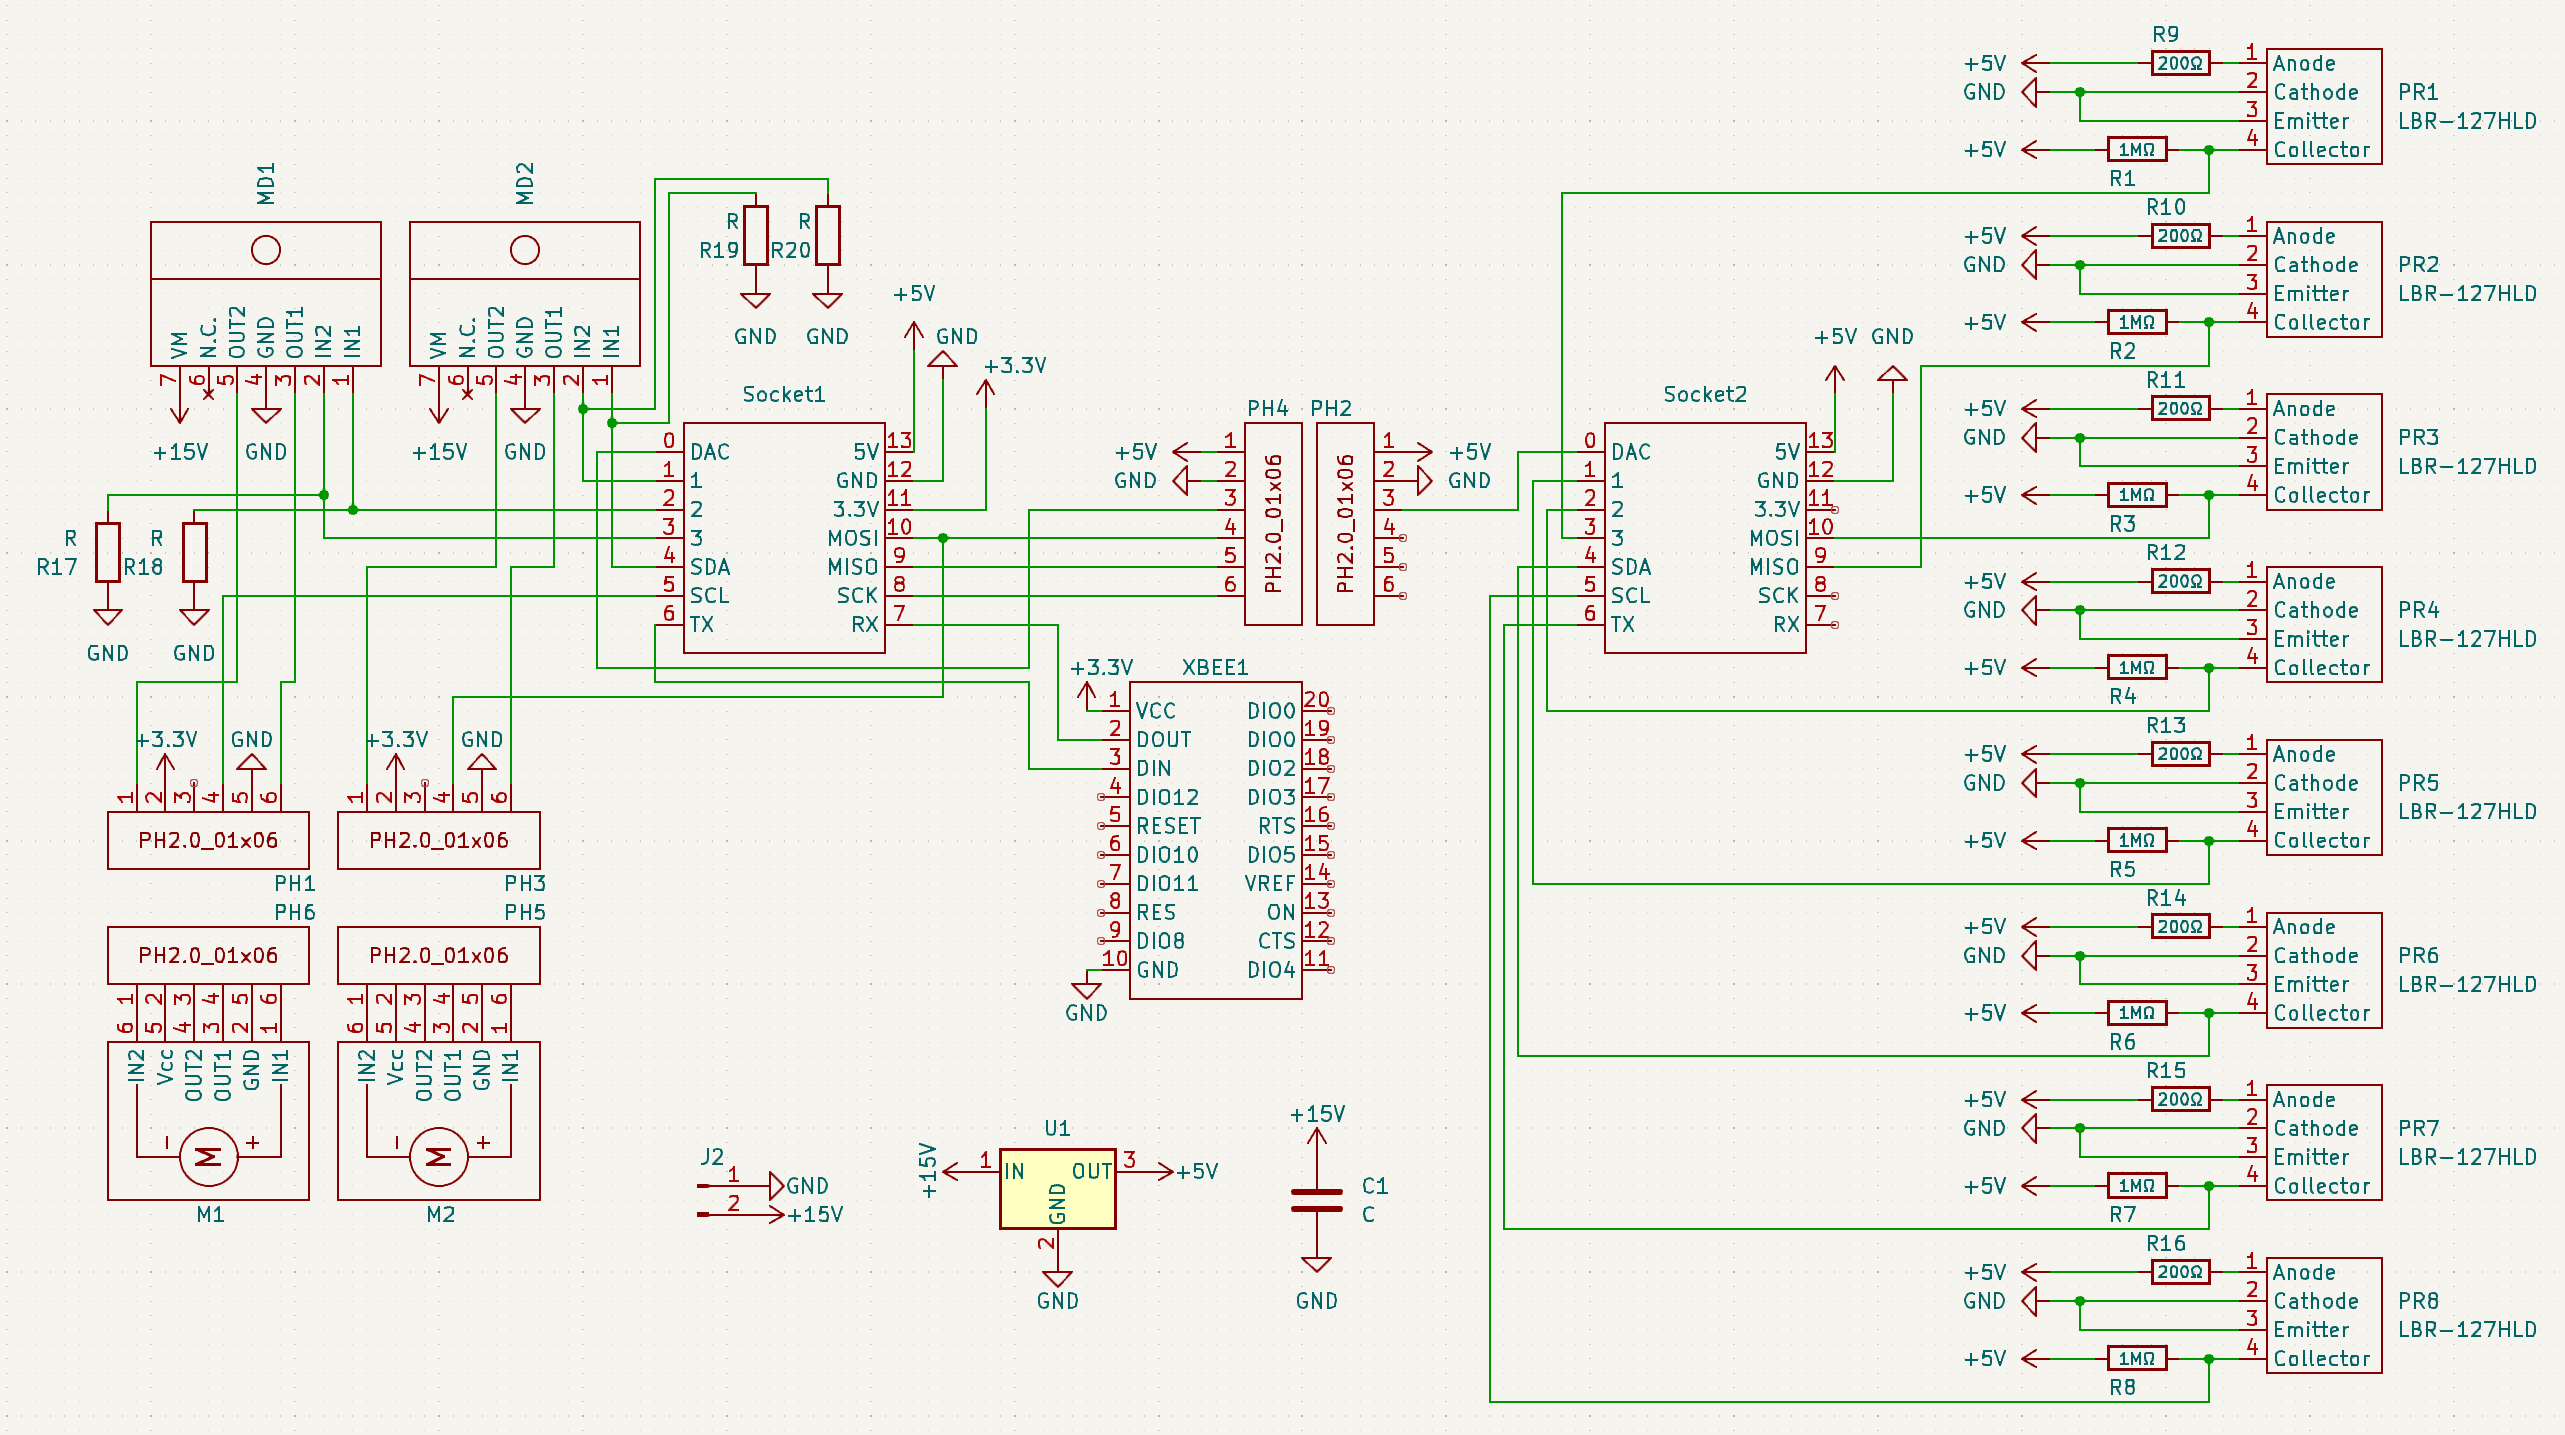
\includegraphics[keepaspectratio, scale=0.35]
       {img/figure_all_circuit.png}
  \caption{回路図}
  \label{fig:circuit}
 \end{figure}

PH2に接続された部分が光センサの基板部分の回路であり、それより左側がメイン基板の回路である。


\section{部品表}
以下に部品表一覧を示す。
モータについては、12 V、ブラケットありの製品で、530RPM(望月氏出資機)、1000RPM(筆者出資機)のものを使用した。

\begin{table}[H]
  \begin{center}
    \begin{tabular}{l|l|l|l|l} \hline
      記号 & 部品名 & 単価(円) & 個数 & 購入先 \\ \hline
      (センサ部) & & & \\ \hline
      PR & フォトリフレクタ & 70 & 8 & \href{https://akizukidenshi.com/catalog/g/g104500/}{秋月電子通商} \\
      R1 $\sim$ R8 & チップ抵抗($\SI{1}{\Mohm}$) & 0.71 & 8 & \href{https://ja.aliexpress.com/item/1005001794062302.html?channel=twinner}{AliExpress} \\
      R9 $\sim$ R16 & チップ抵抗($\SI{200}{\ohm}$) & 0.71 & 8 & \href{https://ja.aliexpress.com/item/1005001794062302.html?channel=twinner}{AliExpress} \\
      MP1 & ICソケット (16P) & 13 & 1 & \href{https://akizukidenshi.com/catalog/g/g100007/}{秋月電子通商} \\
      Socket2 & ICソケット (16P) & 13 & 1 & \href{https://akizukidenshi.com/catalog/g/g100007/}{秋月電子通商} \\
      PH & PHコネクタ ベース付ポスト & 15 & 1 & \href{https://akizukidenshi.com/catalog/g/g112806/}{秋月電子通商}\\
      ユニバーサル基板に実装 & Seeeduino Xiao & 850 & 1 & \href{https://akizukidenshi.com/catalog/g/g115178/}{秋月電子通商} \\
      \hline
      (メイン基板) & & & \\ \hline
      ピンソケットに実装 & Seeeduino Xiao & 850 & 1 & \href{https://akizukidenshi.com/catalog/g/g115178/}{秋月電子通商} \\
      MD1,MD2 & モータドライバ TB6643KQ & 350 & 2 & \href{https://akizukidenshi.com/catalog/g/g107688/}{秋月電子通商} \\
      R1 $\sim$ R4 & カーボン抵抗(炭素皮膜抵抗) 1/4W \SI{1}{\kohm} & 1 & 4 & \href{https://akizukidenshi.com/catalog/g/g125102/}{秋月電子通商} \\
      Socket1 & ICソケット (16P) & 13 & 1 & \href{https://akizukidenshi.com/catalog/g/g100007/}{秋月電子通商} \\
      PH & PHコネクタ ベース付ポスト & 15 & 3 & \href{https://akizukidenshi.com/catalog/g/g112806/}{秋月電子通商}\\
      C1 & 電解コンデンサ(100 \mu F 25 V) & 10 & 1 & \href{https://akizukidenshi.com/catalog/g/g117877/}{秋月電子通商} \\\hline
      (その他) & & & \\ \hline
      機体に実装 & 1セルリチウムイオンバッテリー & 321 & 4 & \href{https://ban.ggood.vip/14ElT}{Banggood} \\
      機体に実装 & エンコーダ・ギアボックス付きモータ & 1805 & 2 & \href{https://ja.aliexpress.com/item/1005005954131759.html?spm=a2g0o.order_detail.order_detail_item.3.cf3b1691UYt6KT&gatewayAdapt=glo2jpn}{AliExpress} \\\hline
    \end{tabular}
    \caption{部品表}
    \label{部品表}
  \end{center}
\end{table}

\section{ベース}
ベースは3Dプリンタを用いて造形されており、材質はPLAフィラメントである。
部品としては本体、センサ部連結パーツ、接地部、その他小部品に大別される。
図\ref{fig:3dmodel}に3Dモデルを示す。

\begin{figure}[tbh]
  \centering
  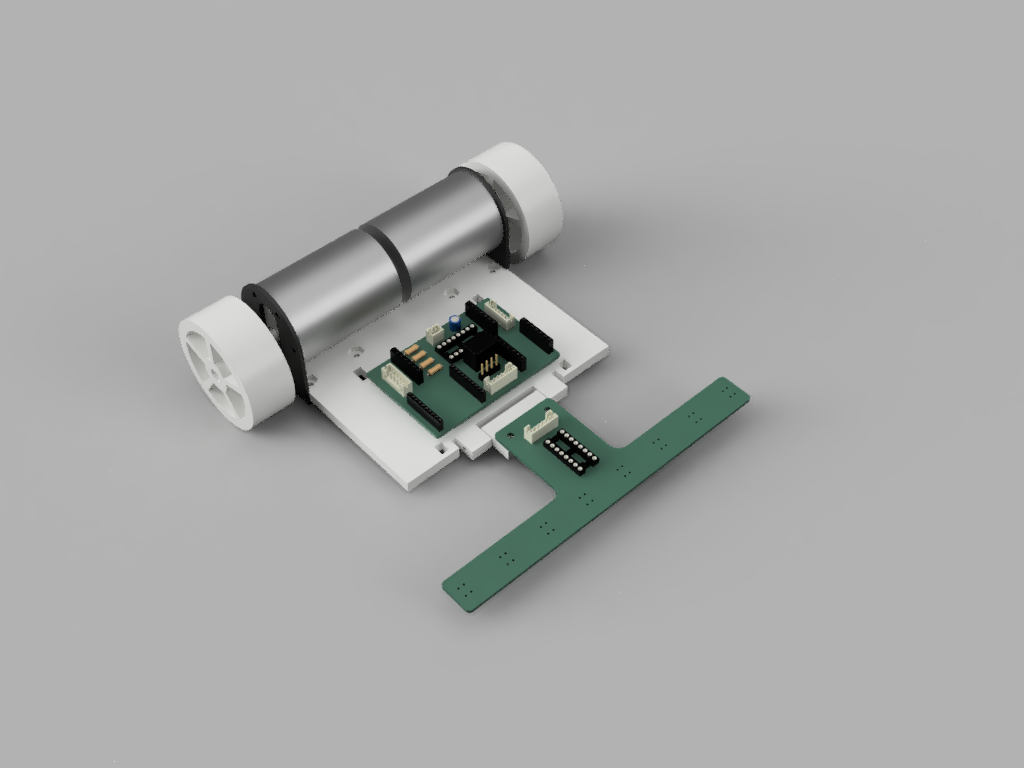
\includegraphics[keepaspectratio, scale=0.4]
       {img/figure_carFramev3_angle.png}
  \caption{ハードウェア設計の3Dモデル}
  \label{fig:3dmodel}
 \end{figure}


\section{光センサ部}
光センサ部は、プルアップ抵抗とフォトトランジスタによる光センサが8個付いており、これらの信号はセンサ用マイコンに送られてソフトウェア的に1つの信号に集約されたうえでメイン基板にアナログ値として送られる。


\section{光センサ拡張マイコン基板}
本来は光センサ出力はマルチプレクサを経由してメイン基板ですべて処理される予定であったが、問題が発生したため、マルチプレクサの部分からユニバーサル基板を生やし、その基板上に別のマイコンを載せて別処理させることになった。
前方にマイコン接続用のUSB Type-Cが飛び出しているため、正面衝突に弱く、拡張マイコンごと外れることもあるため、取り扱いに注意しなければならなかった。

\section{メイン基板}
メイン基板は、光センサ、エンコーダなどすべてのセンサ値を集約し、モータを適切に制御する役割がある。
基板上の役割は電源回路と信号回路に大別される。

電源回路としては、公称値3.8 V のバッテリを4セル直列接続した約16 V の電源と、レギュレータによって5 V に降圧された電源の2種類の電圧が運用されている。16 V 電源はモータを回すために使用し、5 V電源はマイコンやセンサを作動させるために使用されている。
元電源側にコンデンサを並列に挿入してあるため、瞬間的な電圧変動にもある程度の耐性をもつ。

信号回路は、センサ値の取得、マイコンによる制御、モータのPWM制御等に使用されている。



\section{電源基板}
バッテリセルを4つ直列接続するためのPHソケットが並んだユニバーサル基板。すべての電源はこの基板から取られている。スイッチもこの基板に実装されている。










\chapter{ソフトウェア設計}\label{cha:software}
\section{ソフトウェア概観}
%ブロック線図とかこのへんに書く
\subsection{全体構成}
本章ではソフトウェアの構成に必要な理論について説明する。
今回構成した走行体には、光センサとモータのエンコーダという2つのセンサが搭載されていおり、
それらの値をモータの制御に反映したフィードバック制御アルゴリズムを構築する必要がある。
そこで本機ではモータの回転速度を制御量、PWM制御の入力量を操作量としたPID制御を用いることとした。
ただし、一般的にPID制御は1入力1出力の系であるから、光センサとエンコーダという2つのセンサ値のある系ではそのまま
適用することができず、少し工夫が必要となる。ライントレーサの制御には例えばETロボコンについて
の記事~\cite{ETM}が詳しい。これによれば、光センサのPID制御値とエンコーダのPID制御値をそれぞれ計算し、和を取ったものを直接操作量としてPWM制御に入力すればよいとされている。この手法は両方の制御がダイレクトに操作量に反映されるのでよいパラメータを設定できれば非常に応答性が高いプログラムになると思われる。しかし、6つのパラメータを同時に調節する必要があり、走行の様子からどのパラメータをどの程度調節すればよいのかを
見極めるのは初学者には難しい。そのため、今回はセンサ値のPIDから各モータの目標速度を変更し、
その速度に向かってモータ側のPID制御を行うという2段のPID制御を行う方式を最終的に採用した。この方式は、センサ値から直接操作量を変更しないで間にモータ側のPID制御を挟むため、必ずしも最適な速度制御とはならない可能性、およびディレイがある可能性があることが欠点である。
しかし、モータ側のPIDパラメータの調整とセンサ側
の調整を切り離し、1度に3つのパラメータのみ対象として調整することができることがメリットである。
この構成を1つのモータに注目してブロック線図で示すと、以下のようになる。

\begin{figure}[tbh]
  \centering
  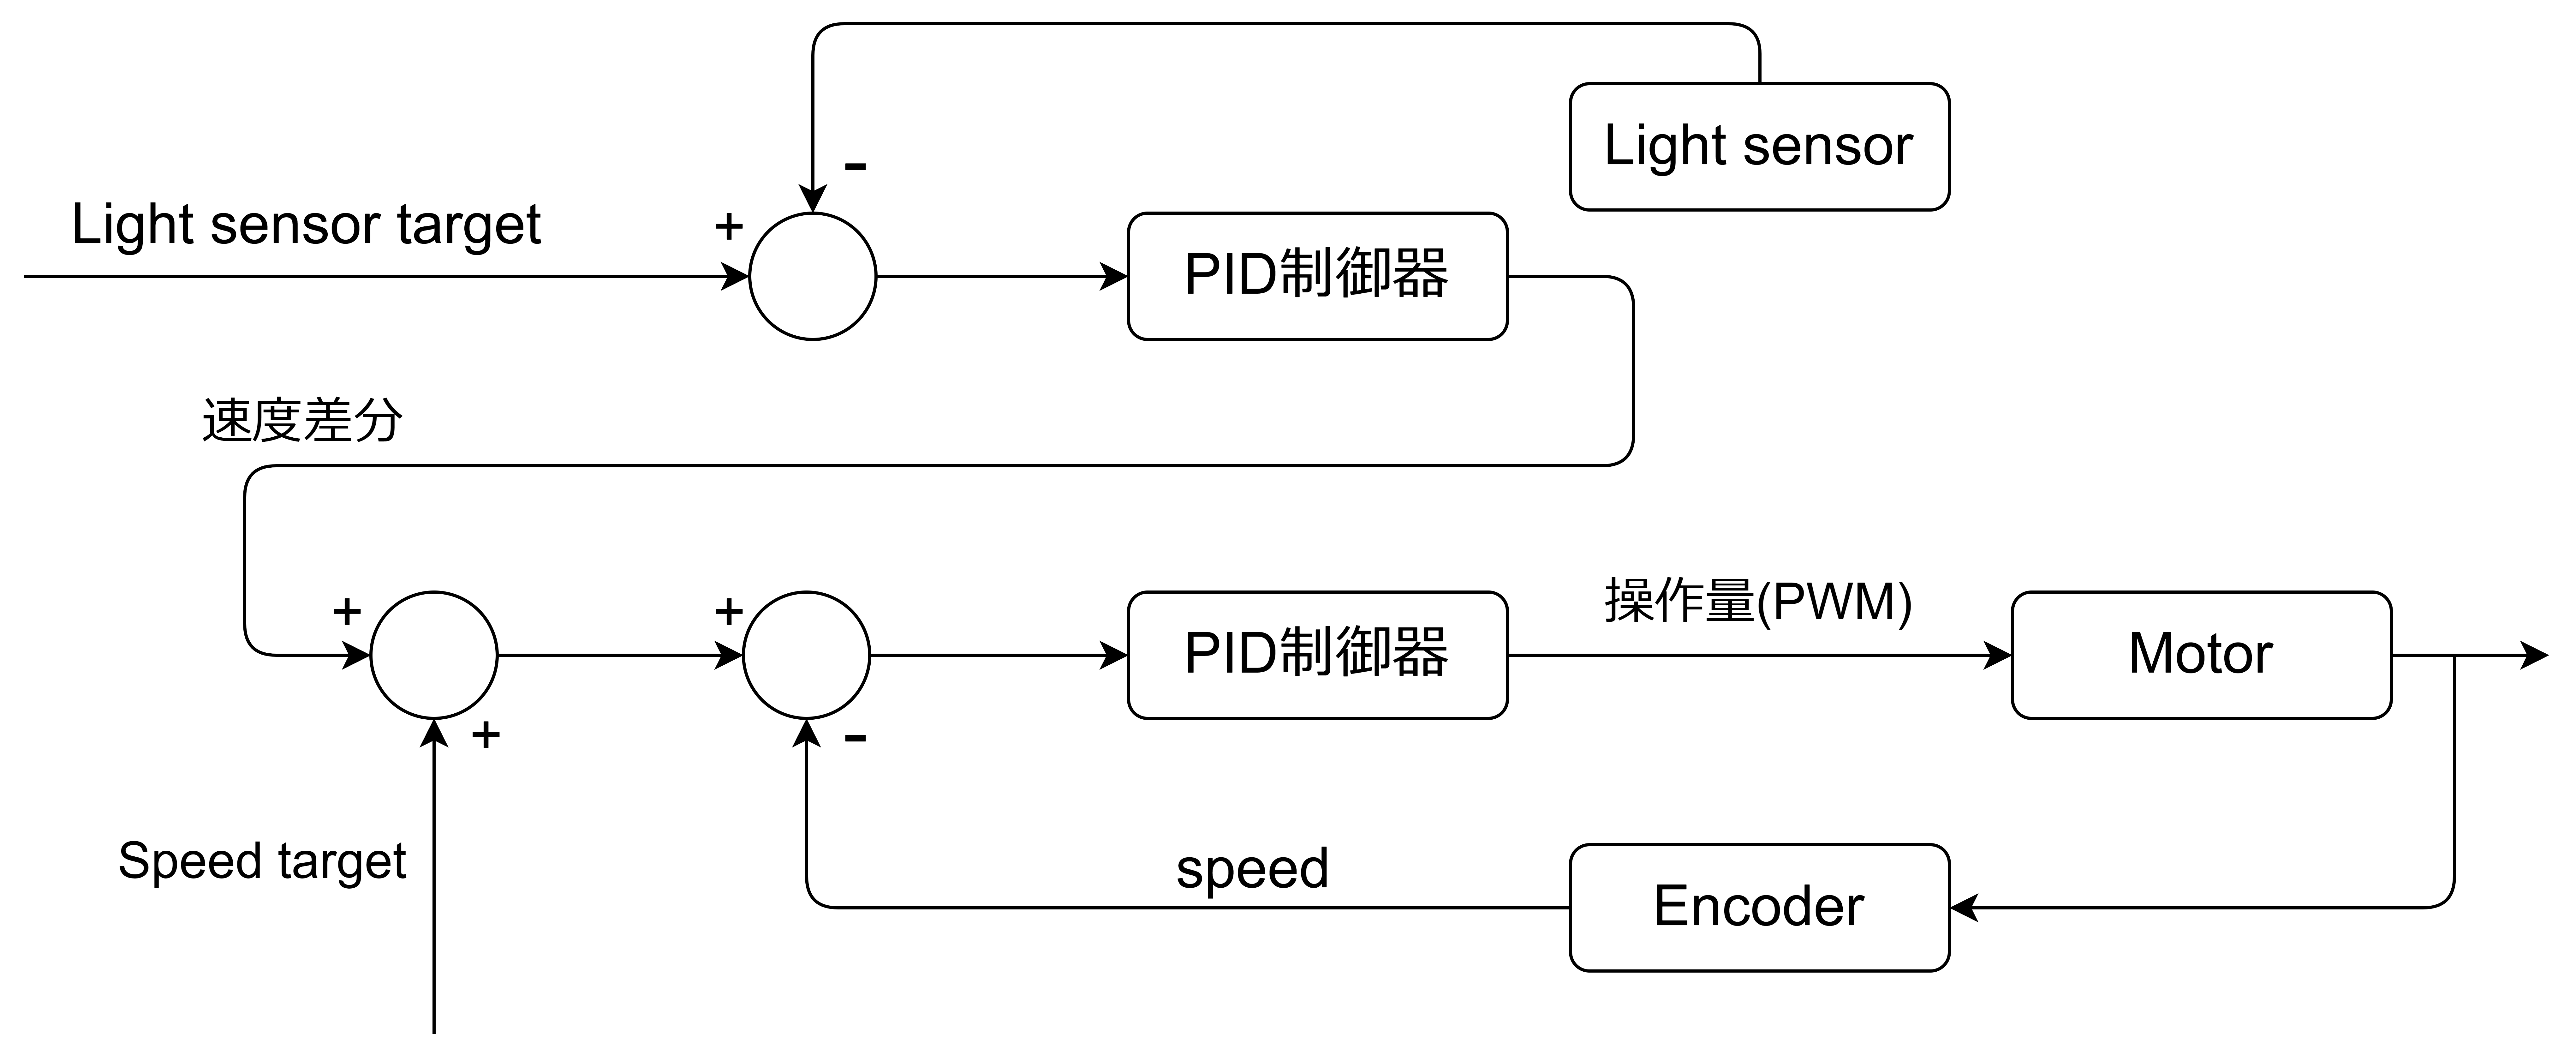
\includegraphics[keepaspectratio, scale=0.05]
       {img/block_line.drawio.png}
  \caption{採用したシステムのブロック線図}
  \label{fig:blockline}
 \end{figure}

PID制御器が2つ直列に接続されていること、および速度のPID制御の前で3つの値の加減算が行われていることが特徴的である。

%制御の具体的な内容は後の\ref{sec:PIDestimate}節から\ref{sec:SensorIntegration}節に記述する。

\section{光センサ値の検出}
\subsection{コース線の中心の推定}
先に述べたように、本機は8つのセンサを積んでいるが、PID制御に回すためには1つのスカラ値に変換する必要がある。センサ値の統合には様々な方法があるが、線が機体の外側に行くほど絶対値の大きい値を返すような単調な関数となっていることが望まれる。
そこで、本機では2つのモータを結んだ線の中心から、コース線の中心と推定される位置の角度をセンサ値として利用する。ここで、コース線が左側にあるとき、負の値を返し、右側にあるときに正の値を返すとする。
位置関係を示すと、図\ref{fig:linepos}のようになる。
\begin{figure}[bt]
  \centering
  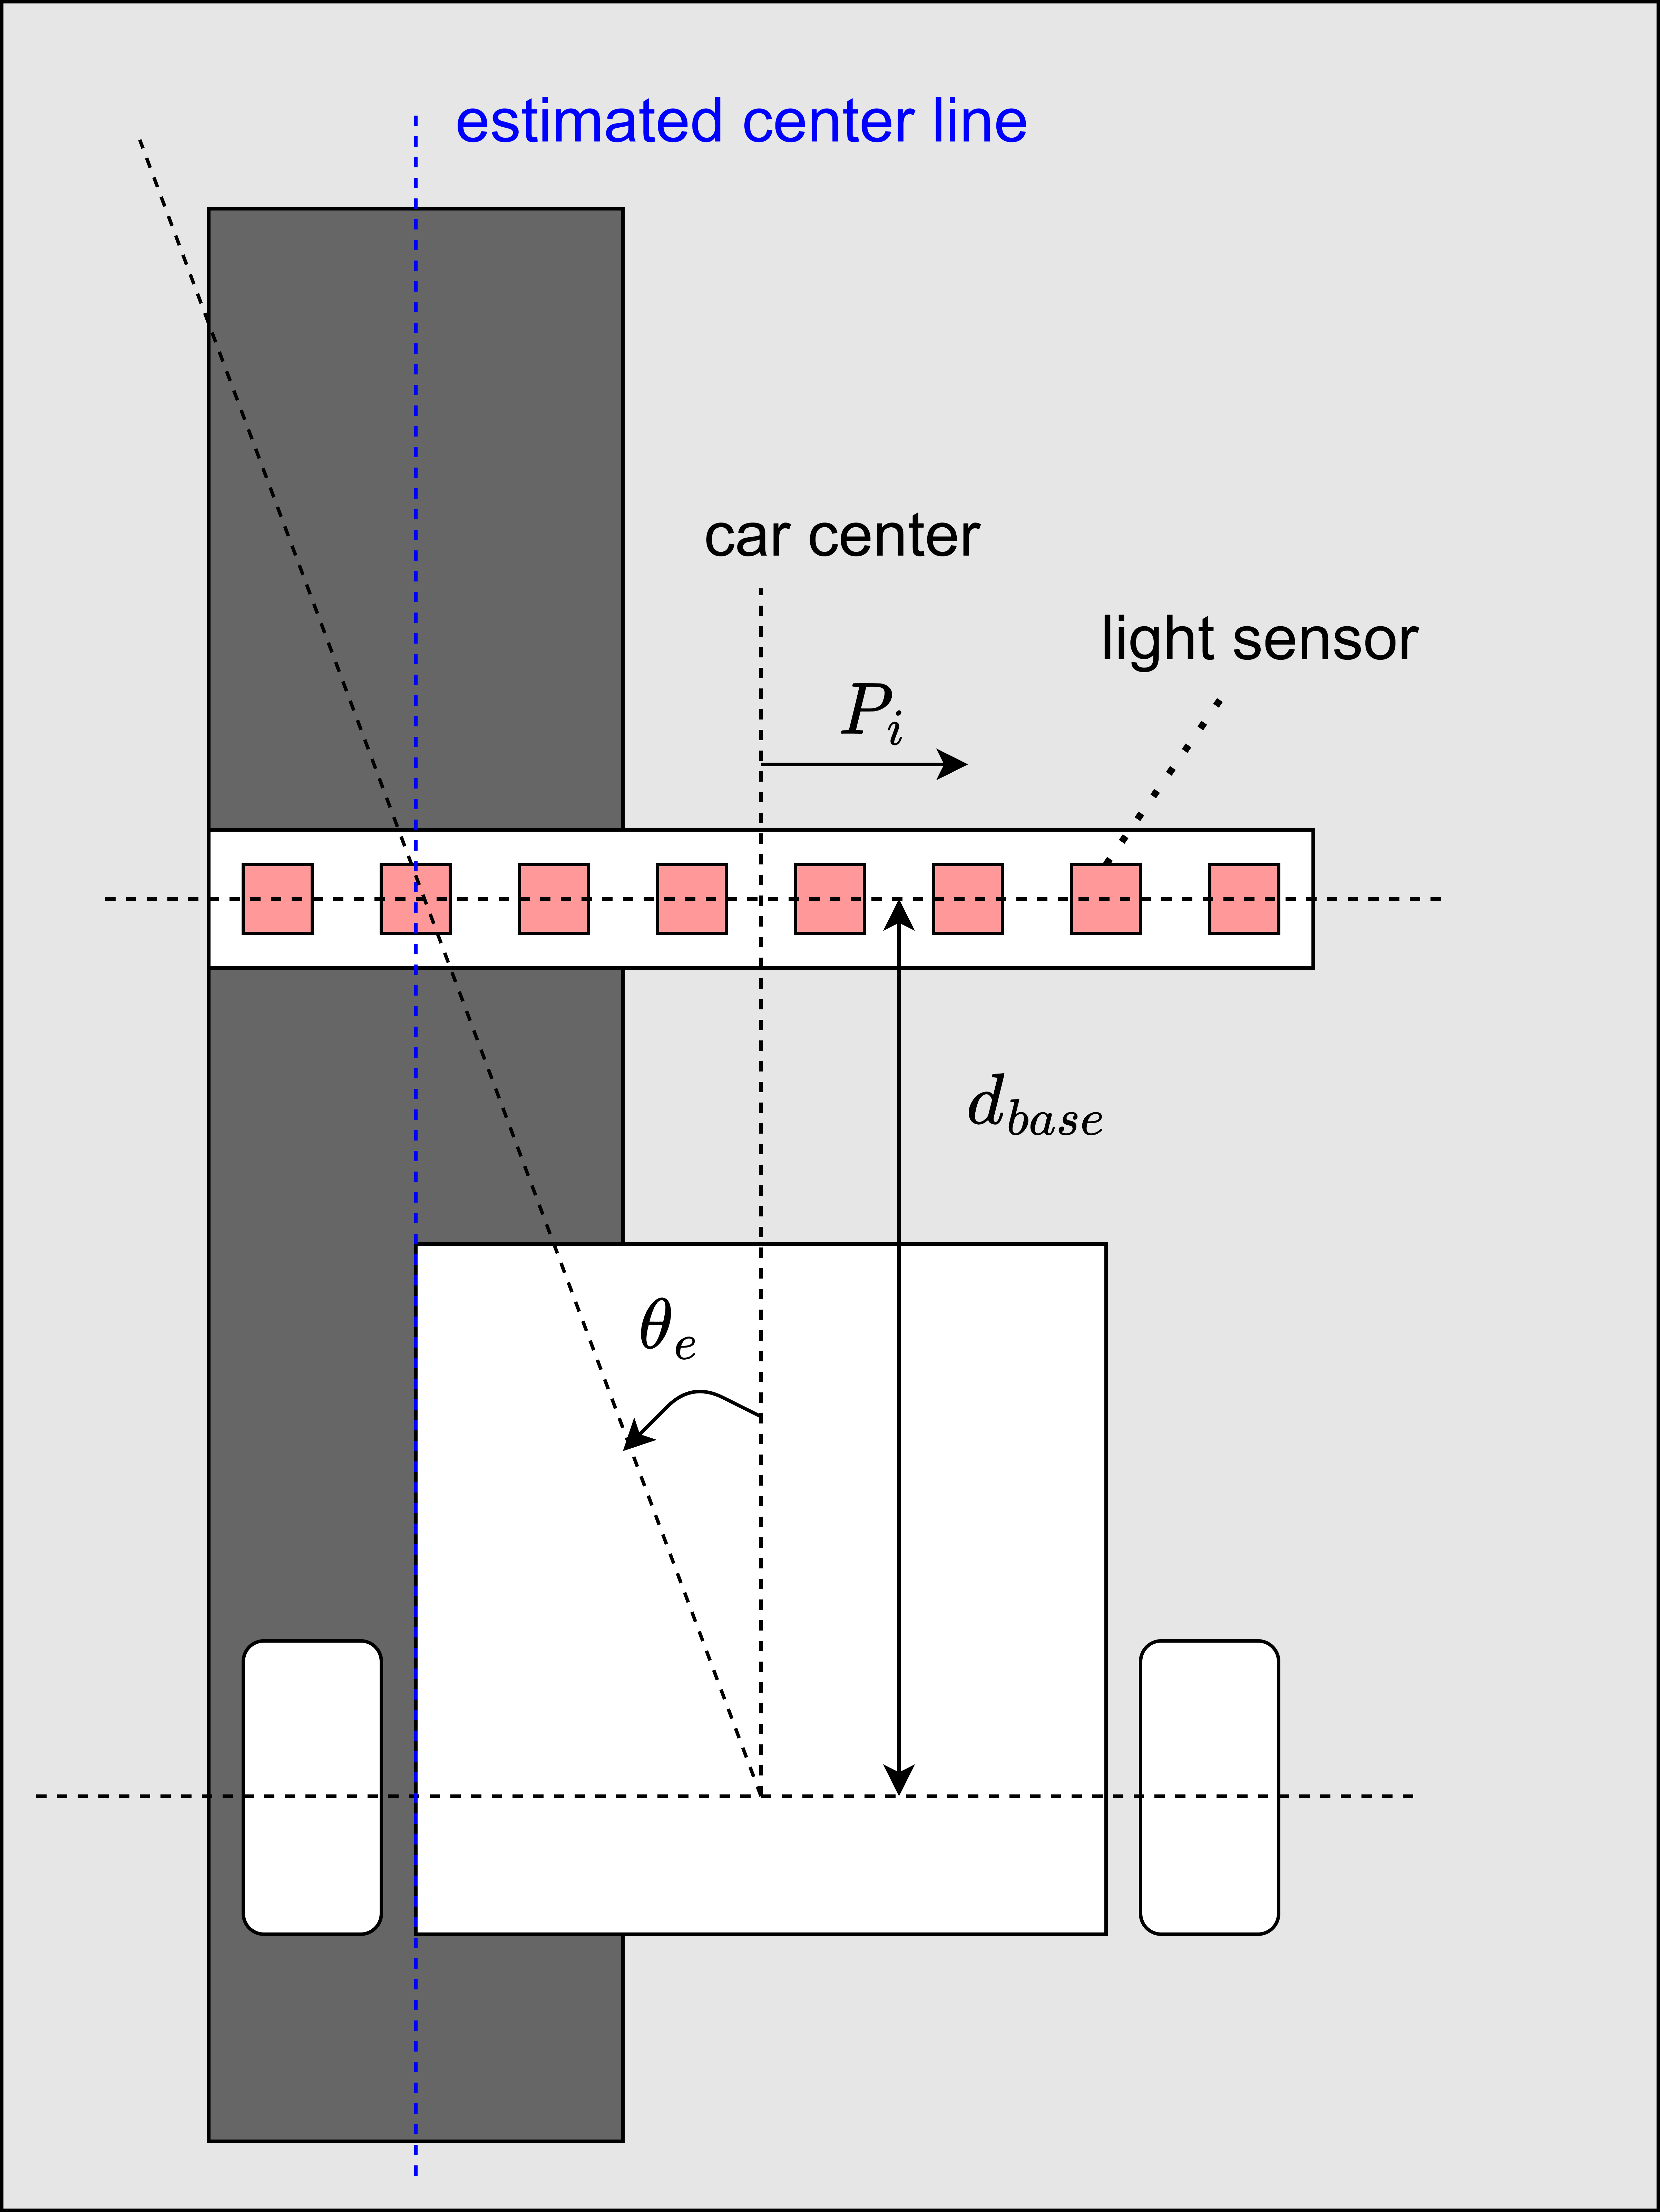
\includegraphics[keepaspectratio, scale=0.05]
       {img/sensor_theta.drawio.png}
  \caption{位置関係}
  \label{fig:linepos}
 \end{figure}


まず、コース線の中心位置を推定する方法を考えよう。
図の左側のセンサから順に0番から7番であるとする。
車体の中心線car\_censorを基準として右側を正、左側を負とする座標系を考えると、
各センサの位置は0番から順に-7, -5, -3, -1, 1, 3, 5, 7 [cm]にある。
つまり、i番目のセンサ位置$P_i$は
\[ 
      P_i = -7 + 2i
\]
である。
次に、センサiがコース線に乗っているか判定する関数を$b[i]$とすれば、

\begin{equation}
  b[i] = 
  \begin{cases}
   1 & (センサiがコース線上にある) \\
   0 & (センサiがコース線上にない)
   \end{cases}
\end{equation}

$b[i]$はセンサの実測値に対してしきい値を付けることで容易に実装することができる。

よって、これらを足し合わせ、``コース線上に乗っている"センサ数Nで割り、平均を取ることでコース線の推定位置$P_e$は

\[ 
  P_e = \frac{1}{N} \sum_{n=0}^7 b[i] P_i
    \]

\subsection{角度の推定}

次に、車軸から見込んだ推定角度$\theta_e$を求めよう。
本機において、車軸とセンサのある位置までの距離$d_{base} = 13 [\mathrm{cm}]$である。また、$\tan \theta_e = \frac{P_e}{d_{base}}$である。
ゆえに、
\[
  \theta_e =  \tan^{-1} \frac{P_e}{d_{base}}
\]
である。

三角関数は計算量が他の演算に対して大きいのでボトルネックとなることがある。その際には、$\tan^{-1}$をテイラー展開して、適当な次数で切ることで冪関数として扱えば良い
\footnote{$\arctan x$のテイラー展開は2次近似まで$x$であるから、大きさの正規化さえ気をつければ$P_e$を直接角度の推定値として扱ってもあまり問題はない。今回は精度を優先した。}。
今回の配置であれば、5次近似程度あれば十分な精度である。
しかし、実際に実験した結果、今回は特にボトルネックにならなかったので、検討はしたものの、特に必要はなかった。

\subsection{読み込みのボトルネック}
以上で8つのセンサを1つのスカラ値に変換することができた。
この処理では8つのセンサを順次読みこむことから、ボトルネックとなり得ることに注意する必要がある。
実は当初設計では採用したマイコンではピンが不足していたのでマルチプレクサを順次切り替えて処理する形式を取っていた。
しかし、実際に試したところ、回路設計の関係なのか、1度切り替えてから電圧が安定するまで110 \mu s 程度要することがわかった\footnote{マルチプレクサ側の問題ではない。モーターのエンコーダも同様にマルチプレクサを使っていたが、3 \mu s程度のディレイで問題なく動作した。}。このディレイは毎回挟むと後述の速度検出のサンプリング周波数が不足するため解消する必要があった。
そのため、本機ではマイコンを2台利用するように設計を変更し、光センサ値の検出に関係する部分をすべて移動した。
遅延への懸念から、光センサ用マイコンから本マイコンへの通信には通信プロトコルを使用せず、適切なレンジにマッピングしたアナログ値(電圧)を出力し、受け取り側で扱いやすい値に再マッピングすることで問題なく利用することができる。
今回は受け取り側で[-10, 10]の範囲に再マッピングした。

\section{速度の検出}
\subsection{エンコーダ}
速度の検出にはモータに付いているエンコーダを活用する。
エンコーダにはホールセンサが付いており、車輪を回転させると、1回転で決まった回数$P$だけデジタルでパルスが送られる。
本機においては$P=11$である。
つまり、信号を$f(t)$とし、モータを定速で回転させたならば$f(t)=1 \; \mathrm{(HIGH)}$となる時間と、$f(t)=0 \; \mathrm{(LOW)}$となる時間を周期的に
繰り返す。
通常モータは正転と逆転を判別するために位相の異なるホールセンサが2つ搭載されている。しかし、今回はモータは逆転しないものとし、1つのエンコーダにのみ着目する。

\subsection{センサ値のサンプリング}
デジタル値が流れている生データから速さを取得するためには、信号の値の変化を捉えてその時間間隔を調べればよい。1つのエンコーダで捉えられる値の変化はHIGH to LOW または LOW to HIGH の2種類である。仮に両方の変化を捉えるとすれば、1回転で$2P$回の変化を捉えることとなる。一般に、より多くの変化を捉えるほうが精度のよい速さが求められるが、サンプリング周波数に注意する必要がある。プログラム中で速度を毎ループ計算せずに非同期で処理する場合、1ループにかかる時間の逆数がサンプリング周波数である。
そして、1ループで1回の変化が起こる状態(毎回のループでHIGH -> LOW -> HIGHと変化している状態)が取得しうる最高速度であり、それ以上の速度は測定できない。しかし、そもそもナイキスト定理を考えれば、この状態はすでにエイリアシングが発生して精度が低下しているから元の信号の周波数は更に低くなければいけない。さらに言えば、ナイキスト定理では2倍のサンプリング周波数があれば良いことになっているが、波形を復元する特別な工夫がないなら10倍以上の周波数を使うべきである。
フーリエ変換を考えて厳密に言えば、デジタル信号は矩形波であるから、無限大の周波数がなければ修復できない。そのため、どのようなサンプリング周波数で計測しても、たまに飛び値が出る。しかし、モータは瞬間的に追従することはできないうえ、次の瞬間には正しい値に戻っていることを考えれば飛び値が出ることは問題にならない。そして、LOW->HIGH->LOWをあたかも1つの波であるかのように捉えてその周波数を考えてみればこの計測法でも比較的正しい速度が計算できることがわかる。こちらで考えても周波数が高すぎるときは、変化の読み落としが発生しているので全く信用にならない。本機ではLOW to HIGHのみを捉えることとする。

ここまでは、非同期で処理する場合を考えた。では同期処理ではどのような問題があるだろうか。
まず、同期処理では毎回の処理でそのときの速度を定める。つまり、毎回速度が確定するまでこの処理のみを実行するので、読み落としは発生せず、エイリアシングの問題等は一切考える必要がない。ここだけ聞くと、同期処理のほうがよく聞こえるかもしれないが、問題はこの処理が終わる(= エンコーダの変化を2点で捉える)まで次の処理に進めないことである。高速走行時には短い時間で変化を捉えられるので大きな問題にはならないかもしれないが、低速時には待ち時間が増えるし、停止時には停止しているかどうかを明確に判別できるだけの最大待ち時間待たなければならなくなる。その時間はモータに依存するが本機においては最低でも20msであった。つまり、1ループに最大20ms、高速走行時でも非同期処理よりは当然遅く、数msの待ち時間が発生する。待ち時間とはつまり制御が入らずに空走する時間である。例えば、50cm/sで走行中に5msの待ち時間があったとすると、空走距離は50cm/s \times 5ms = 0.25cmである。僅かな量に感じるかもしれないが、これだけの空走距離があると急なカーブ等には対応することが困難である。つまり、同期処理で速度を取得すると非常に大きなボトルネックになるので、速度の計算は非同期処理にする必要がある。


\subsection{生データから速さへの変換}
前節でモータ1回転に捉える変化数を決めた。改めて$P$とおく。つまり、本機においては$P=11$である。
次に、値の変化にかかった時間を$\Delta t$ [\mu s] とする。モータのギア比(減速比)をRとする。タイヤの直径を$D$ [cm] とすれば、タイヤ外周部の速度$v$ [cm/s]は次の
ように表される。
\[ v = \frac{\pi D \times 10^6}{R P \Delta t} \]

これは実質的に時間の1変数関数であり、残りは機体に固有の定数であるから、切り分けて前処理に回すことで処理を高速化できることに留意したい。
また、車体が停止しているとき、$\Delta t$は永遠に求まらないため、同期処理と同様に一定時間経過したら速度を0と判定するしきい値時間を用意する必要があることに注意する。

\subsection{非同期処理の実装}
本機はArduino互換ボードを使用しており、ソフトウェアの実装言語はArduino言語である。そのため、Python等高機能言語に実装されているasync/await等の高級な非同期処理インターフェースはない。
そのような状況でシンプルに非同期処理を実装するためには、時間を確認することが有効である。Aruduino言語には、経過ミリ秒を表示するmillis()やマイクロ秒を表示するmicros()が存在するため、それを用いることで素朴な非同期処理を実装することができる。

その他の選択肢としては、今回は採用していないが割り込み処理にする方法が考えられる。
ボード依存であるが、Arduinoは割り込み処理をサポートしている。ホールセンサの信号の変化をトリガとした割り込み処理をすればより
無駄のない速度計測ができる可能性がある。
\subsection{ノイズ対策}
エンコーダでは、ホールセンサの信号をHIGHとLOWで送信する。回転の途中で値の境界付近の状況にあるとき、短い周期で信号が震えることがある。これはスイッチにおけるチャタリングに近い現象であり、同様に対策が必要となる。
本機では、信号値を取得する際に毎ループで続けて3回取得し、すべての信号値が揃わなければ信用できないとして信号を取得し直す、というロジックによりこの問題へ対処した。



\section{モータ制御}


\subsection{センサのPID制御}\label{sec:SensorIntegration}
これまででそれぞれのセンサ値を取ることができた。次にこれをモータの動作に落とし込む必要がある。
用いるPID制御を時間の式で示せば、
\[
  y = K_p e + K_i \int e \; dt + K_d  \frac{\mathrm{d}e}{\mathrm{d}t}
\]
ただし$e$は目標値から現在値を引いた偏差である。
これはアナログ値であるから、デジタル値による記法に変換する必要がある。これにはいくつかの流儀があるが、今回は最も基本的な方式として、微小時間は無視する、積分要素は面積を取らずに現在差分を単純に足す、微分要素は差分要素に置き換えるという方法を取った。


今一度PID制御器の結果がどのように使われるか確認すると、
光センサについてのPIDの結果は曲がる方向に応じてモータの目標速度を変化させる役目をもつ。
モータについてのPIDの結果はもちろん所望の目標速度に近づくようにモータへ送る操作量を調整する。

%本機体において、センサ値は、メインとは別のマイコンで処理されて送られてくる。送られてきた値は処理しやすいように、[-10, 10]の範囲にマッピングするものとする。
図\ref{fig:blockline}にブロック線図を示してあるから、あと必要なことはそのまま実装して、パラメータの調節を行うことのみ(これが一番大変かもしれない!)である。

\subsection{光センサにおけるPID調整前のパラメータ推定}\label{sec:PIDestimate}
PID制御のパラメータ調節は地道な作業であるが、論理的に考えられる部分については、ある程度あたりをつけてから始めると楽である。
特に、PID制御の調節はP制御から始め、$K_p$の大きさによって他の値のレンジの決定されるので、$K_p$の正当性が最も重要である。
ここでは、光センサのP制御値について考察を行うことでパラメータにあたりをつけてみよう。

ライントレースを行ううえで一番走行が難しいのは急カーブである。逆にいえば、急カーブを走行してもコースアウトせずに即座に車体の安定を取り戻せる状態なら他の場所は問題にならない。では$K_p$をいったいどのくらいの大きさにすれば最も急なカーブを曲がり切れるだろうか?

最も急なカーブの曲率半径を$r$[cm]とする。車体の中心線からタイヤの中心までの距離を$d$[cm]とする。与えた走行速度目標を$v_t$[cm/s]とする。ここで、走行速度目標とはカーブに差し掛かって光センサ値による補正がかかった値ではなく、光センサ値によらない(つまり、直進中の値とも言える)である。
ある瞬間、走行体は角速度$\dot{\theta}$[rad/s]で円運動をしているとしよう。このとき、機体の制御により、外側の車輪の目標速度は$v_t + \Delta v$、内側の車輪の速度は$v_t - \Delta v$に変更される。ただし、$\Delta v $は$K_p$に依存する値である。このとき、速度に関する次の2つの式が成り立つ。

\begin{align}
  v_t + \Delta v &= (r+d)\dot{\theta}\\
  v_t - \Delta v &= (r-d)\dot{\theta}
\end{align}
ここから$\dot{\theta}$を削除することにより、
\begin{align}
  \frac{v_t+ \Delta v}{v_t-\Delta v} &= \frac{r+d}{r-d}\\
                                    &= k
\end{align}
とおくと、$k$は$r$と$d$によって決まるからコースと車体のプラットフォームが変わらない限り定数である。
このkを用いると、
\[
  \Delta v = \frac{k-1}{k+1}v_t
\]
と表される。つまり、光センサのPID制御全体で$\Delta v$ より大きい速度の変化分を出せないと曲がりきれないことが実験しなくてもわかる。

本機体について考えてみよう。
本機体において、$d=7.5$[cm]
速度$v_t =100$[cm/s]で、曲率半径$r=10$[cm]の円を曲がるとする。このとき、$k = 7$であるから、
$\Delta v = \frac{6}{8}v_t = \frac{3}{4}\times 100 = 75$である。
いま、光センサ値が[-10, 10]の範囲でマッピングされている。現在の光センサの値を$l$とする。
光センサの目標値は中心である0とすれば$e=l$。ここでの偏差は定義とは反対であるが、その後のデータの与え方を反転させれば問題ない。絶対値で扱っていると考えても良い。
P制御しか行わない状態を仮定すると、$\Delta v = K_p |l| > 75$となる。
光センサが最大値のときにぎりぎり曲がりきれると仮定すると、$l=\pm 10$で、$K_p > 7.5$となる。
実際にはもっと余裕を持ちたいのでより大きな値となると推定される。
たとえば、$l=8$で曲がりきりたいとすると、$K_p > 9.38$程度となる。
これとD制御を組み合わせることで、急なカーブでもより安定して走行することができる。

実際に採用した値が$K_p=10.0, K_d = 12.5, K_i = 0.0002$であることを考えるとこの考察は非常に有益であることがわかる。



\subsection{アドホックな調整}
%ダンパーとsk
ここまでで、カーブを含めたほとんどの場合において安定した走行をするための議論は完了した。
しかし、まだ特殊な場合で安定しない可能性が残されている。本節ではそのような特定の状況に対応するアドホックな処理について議論する。

安定しない可能性があるのは速度0からの立ち上がりの状況である。
理由は2つある。

1つ目は、目標速度を大きくすればするほど、初めのP制御が強く効くからである。
理想的状況であれば、速やかに目標速度に到達するため問題ない。しかし、左右のモータの回りやすさに差がある場合、初めの制御量が大きく入ると左右差が大きく出やすく、場合によっては修正する間もなくコースアウトしてしまう。

これに対応するためには立ち上がりの偏差に制限をかければよい。つまり、両輪が低速時に限り、現在速度から逆算したターゲット速度を与えることで実現される。これは、数式モデルとしては異なるが、一次遅れ要素に似た性質をもつ。
つまり、以下のようにすればよい。
\begin{verbatim}
  DelayAccelerationSpeed(targetSpeed, maxError, leftCurrentSpeed, RightCurrentSpeed)
    if leftCurrentSpeed < threshold and rightCurrentSpeed < threshold
      newTargetL = min(leftCurrentSpeed + maxError, targetSpeed)
      newTargetR = min(RightCurrentSpeed + maxError, targetSpeed)
      return newTargetL, newTargetR
    else
      return TargetSpeed, TargetSpeed
\end{verbatim}
副次的効果として、偏差の最大値が部分的ではあるが制限されることになるため、モータ側のPID制御の$K_p$をより大きくしても問題が起こりにくくなる。すべての場合で偏差の最大値を制限すれば偏差がmaxError以下であることが保証されるのでそれを念頭に置いた設計ができるが、急カーブを曲がりにくくなるという難点があるため推奨しない。

安定しないもう1つの理由は、センサのPID制御値の速度依存性である。
\ref{sec:PIDestimate}節で速度に応じて与えるべきセンサの$K_p$が変化することを述べた。
もちろん$K_p$は目標速度に合わせて作られているから、立ち上がりの速度ではいささか強く効きすぎる。
そして、先に述べたように、モータには個体差があるから同じように操作量を与えてもまっすぐに進み出すわけではない。
その結果、低速でラインを跨ごうとし、一方の車輪が完全に止まろうとする、逆向きに曲がろうとしてもう一方の車輪が完全に止まろうとする、という動作を繰り返して、振動的な挙動をしながら加速する。このような挙動ではスムーズな立ち上がりとは言えないから、対処したほうがよい。

これに対応する解決策も単純であり、両輪が低速であるときにはセンサのPIDの係数を書き換えれば良い。
もちろんなめらかに変化させることもできるが、低速用の係数を用意して、書き換えるか、書き換えないかという2段階があれば十分であると思われる。
本機の場合は、50cm/sにチューニングしたPID値を用意して二段階にしておけば十分安定した走り出しとなった。

\subsection{Xbeeとの通信}
低速で走行実験を行う場合、万が一コースアウトしても手で止めに行けば問題にならない。
しかし、100cm/sといった高速で走行する場合、手で止めると機体にダメージが入ったり、手で止める前に壁に衝突する危険性がある。
走行会の前に事故によって機体が破損するといった事態は絶対に避けなければならない。
これを避けるため、遠隔で発進と緊急停止を行うことができる機能があるとよい。
やり方は様々あると考えられるが、本機ではXbeeを搭載して遠隔シリアル通信による発進と停止の機能を実装した。


\section{ソースコード}
長くなるので、GitHubのリポジトリと、
付録\ref{cha:code}に添付している。

GitHubリポジトリのリンクは\url{https://github.com/RiceCake1/LineFollow/tree/main}.

この節では、実装を関数別に簡単に解説する。
なお、Arduinoではデフォルトでsetup関数とloop関数が必要である。
setup関数は起動時に1度だけ呼ばれる関数であり、ピンの設定や、初期化等を書く場所である。
loop関数はsetup関数のあとに常に呼ばれる関数であり、メインループとなっている。

\subsection{光センサ関係(光センサ用ボード側)}
\subsubsection{float ReadSensorBinary(int sensorNum)}
センサがコース線に乗っているか判定する関数。

\subsubsection{float ReadSensor(int sensorNum)}
アナログ値を読み[0,1]にマップして返す関数。デバッグ用。

\subsubsection{int getLinePos()}
以前使われていた、センサ値の統合アルゴリズムv1。

\subsubsection{float getLinePosThetaWeighted()}
以前使われていた、センサ値の統合アルゴリズムv2。
角度を考慮し始めた。
試行錯誤の痕跡。

\subsubsection{float getThetaWithArctan()}
最終的に採用された、センサ値の統合アルゴリズムv3。
解説した通り単調な関数となっていて、非常に安定性が高い。
これに変更してからカーブ後の振動の収束が有意に早くなった。

\subsection{光センサ関係(メインボード側)}
\subsubsection{float getLinePos()}
メインボード側で光センサ処理用マイコンから送られてきた値を読み、[-10.0, 10.0]の範囲に再マップする関数。
\subsubsection{float getPIDsensorValue(int linePos)}
光センサのPID制御値を計算し、返す関数。
低速時に係数を変更するアドホック処理も含まれている。



\subsection{エンコーダ関係}
\subsubsection{int \_smoothEncoderSignal(int encoderNum)}
ノイズ対策として3回エンコーダの信号を読み、すべて一致するまで繰り返す内部関数。
\subsubsection{bool \_isChanged(int encoderNum)}
信号が変化したかを判定する内部関数。
\subsubsection{float \_getSpeedWithTime(int motorNum)}
1つのモータについて非同期処理で速度を取得する内部関数。
\subsubsection{void getSpeedWithTime(float *spd)}
上の関数を用いて両輪の処理をまとめた関数。
\subsection{モータの制御関係}
\subsubsection{void controlMotor(float Rspeed, float Lspeed)}
[-1,1]の値の2引数を取り、両輪のPWM制御を簡単に行う関数。
負の値ならば後退、正の値ならば前進。
本番環境では内部関数だが、デバッグ用途ではそのまま使える。

\subsubsection{void delayAccelerationSpeed(float targetSpeed, float *newTargetSpeed, float maxError = 10)}
アドホック処理のための関数。
立ち上がりの速度偏差に制限をかける。

\subsubsection{void controlEachMotorWithPID(float rightTargetSpeed, float leftTargetSpeed)}
左右モータの目標速度をそれぞれ引数に取り、PID制御値を計算して、controlMotorでモータを制御する。

\subsubsection{float limitSpeedOnCorner(float targetSpeed, float deacceleratedSpeed, int linePositon)}
終盤に作られた失敗作。コーナーでは両輪とも減速すれば平常時の目標速度が速くても曲がり切れるのではないだろうか、という仮説に基づいて作られたアドホック制御関数。実際には、この関数が働き始めるときにはすでにブレーキには遅すぎる地点であることがわかった。
消されたものも多いが、このプロジェクトにはこのような不採用になった関数が山程存在し、その数だけ試行錯誤があった。
参考までに、最終形である現在ではメインボードのコードは280行程度であるが、一時期は500行以上あった(1月20日のコミット)。

\subsubsection{void controlMotorFromSensors(float targetSpeed, float deacceleratedSpeed=10)}
最終的に採用されたすべてが集約された関数。
センサ値の取得、光センサのPID制御値の計算、モータのPID値の計算、モータへの操作量の入力までがすべてこの関数で繋がった。

\subsection{その他}
\subsubsection{float mapFloat(float InputValue, float InputLower, float InputUpper, float OutputLower, float OutputUpper)}
ある範囲内の実数を別の範囲にマッピングするための関数。

\subsubsection{show...()}
show関数系は名前が示すものをシリアルで表示するデバッグ用関数。

\subsubsection{initAll()}
名前の通り、変数の初期化等をまとめている関数。
setupで実行するほか、Xbeeで停止させていた走行体を再び走行させるときに実行される。

\subsubsection{Xbee()}
無線通信を行い、ソフトウェア的に停止、発進を行うための関数。
高速でのデバッグでは壁に衝突するなど事故が乱発していたため、必ず機体を緊急停止できる人員を配置し、その人の許可\footnote{電源を入れると発進する状態のときに``Cleared for run"の合図。後に電源を入れても自動で発進せず、管制官が発進信号を送るように変更された。}なく発進させてはいけないという管制塔システムを導入した。
その結果安全性が向上し、機体を破壊することなく無事本番を迎えられた。




\chapter{評価}\label{cha:eval}

\section{ループ速度}
1ループがどの程度の時間で回るか、というのはよい制御をするために非常に重要である。
ボトルネックが大きかった当初、1ループは8\~20 ms 程度であった。
最終的には1ループが203 \mu s 程度となり、10倍以上の高速化が達成された。

\section{実測記録}
530RPMのモータを使用した機体では59秒、1000RPMのモータを使用した機体では65秒であった。
同じ速度ではローギアのモータの方が安定すること、およびチューニングにかけた時間が前者の方が長いことを考えれば妥当な結果であある。
\section{感想}
この実験はライントレーサをフルスクラッチで製作し、爆速で走行させるという高い目標をもって始まりました。
小中学生の頃に電子工作をかじっていて、基本的な回路の理解があり、プログラムも普通に書ける私(と望月氏)にとっては既製品の機体を少し改造して走行させるというのはある意味当たり前にできることだ、という前提があったからです。
無論、昨年まではラズパイとev3を用いるという制約があったので今年もそうであればここまで野心的な実験にはならなかったと思います。
第一回目の授業で先生が、昨年と違ってすべて部品について自由で、何が必要か(そして、何が学びになるか)を考えて始めてほしい、という旨と情報共有は自由という旨が説明されたときから、望月氏とタッグを組んでこのプロジェクトは始まりました。

両者ともにソフトウェア、ハードウェアの両方ともある程度扱える素養はあれど、
私はどちらかというとソフトウェア寄りの研究をこれまでにしていて、数学などを活用して理論的に考えていくことが得意なのに対し、望月氏はハードウェアの研究をしていましたから、ハードウェア側の設計は望月氏の方が長けていました。
それゆえ得意分野が相補的な関係になっていたことはチームを組むうえで非常にメリットだったかと思います。
私達が春学期に取っていた実験はどちらも複数人で進めるものでしたので、複数人で作業するのは実験の目的のひとつだろう、と思っていたし、オンライン世代というのもあるのですが、10人もいるのにお通夜のような雰囲気の実験教室を非常に心配していましたから積極的にコミュニケーションが図れるように画策していました。
ほぼ全員参加のdiscordを作ったり(これはあまり活用されなかった)、手が止まっている人や机がきれいな人に声をかけて困りごとがないか聞いて回ったり(これはかなり有効で、いろいろ出てくる。ハードウェアの知識のない人が自由にしろ、壊すなと言われると何を調べるべきかもわからないというのはあたりまえ。質問をしに行くのも最初のうちは何を質問していいかわからないので難しい。)しました。効果の有無はわかりませんが、最終的には割と会話も生まれ、全員完成できたことは素晴らしかったと思います。

少し話題が逸れましたが、このような背景があるため、私がこの実験を通じて学ぼうとしたことは、もちろんハードウェア寄りです。
具体的には、知識として、大学レベルの電気回路の知識、制御工学の基礎について。
そして、実践として、回路の設計やこれまで経験のないSMDのはんだ付け、カシメ工具でPHコネクタを通すなどの作業などです。

この中でも電気回路の知識は非常に身につけられたと思うので、紙面を割いて電気回路の解説を書いてみました。
理解をしていても自分で解説を書くのは存外難しく、導入があまり美しくないほか、計算を省略しがちなので対象が初心者とも上級者とも言い難い微妙な仕上がりになってしまったこと、書こうと計画していた部分まで書き上がらなかったのは反省点です。
制御工学も軽くは勉強したのですが、解説できるほどではなかったことと時間が足りなかったので解説は書きませんでした。

これらの知識を前提として、機体の設計はできています。
私のスキル的にはハードウェアよりもソフトウェアのコントリビューションが多いですから、このレポートではハードウェアの部分は比較的少ないページ、ソフトウェアの部分は重点的に解説しています。

次に、本体に関する反省点なのですが、レポートを書くためにソースコードを整理していたらいくつか大きなバグが見つかりました。
1分切りというかなりの好成績でコースを走破したあの機体なのですが、実はまだ本領発揮していなかった可能性があるようです。
走行会後にこれが見つかったことだけが惜しい点でした。
ほかには、元の設計どおりではうまく動かず、設計が度々変更されながらユニバーサル基板が増えていったことも反省点ではあるのですが、これは初めてのロボット製作であることを考えると致し方ないかと思います。

最後に、私事でございますが、このレポートは大学院飛び入学予定の私にとって学部最後のレポートになります。
そのため、記念としてかなり本気を出して書きました。
非常に長いことで先生に手間を取らせて申し訳ありませんでした。
ここまでお読み頂きありがとうございました。

















\bibliography{reference}
\bibliographystyle{junsrt}




\appendix

% \chapter{応用的な電気回路解析}
% \section{4端子回路}

% \section{ひずみ波交流の解析}

% \section{三相交流}

% \section{分布定数回路}


\chapter{設計の変遷}
本付録では、最終成果物に至るまでの設計の変遷を示す。

\section{零号機}
すべてev3を用いて授業初日に作り上げた機体。
ev3の性能評価のために使われた。
この機体の評価により、初日にしてev3を一切使わない設計に移行することを決定した\footnote{もちろん、そのほうが勉強になるという事実が後押しした。}。

\section{初号機}
10月中に作り上げた実験機。
図\ref{fig:b_machine}のように、配線はブレッドボードとジャンパ線、固定はマスキングテープ、土台にいくつかのレゴパーツ、
センサは本番機同様のもの、モータはエンコーダなしギアなしのDCモータを直接搭載したプロトタイプである。
加速力は非常に低いが、フィードバック制御がないため直線で際限なく速度が上がって次のカーブを曲がりきれずコースアウトする。一方でカーブが連続する地形では普通に走ることができた。
回路設計はこの機体のときにほぼ確定した。
問題点を洗い出し、設計の原型を形作ったという点で非常に重要な役割を果たしたプロトタイプである。
これ以降は徐々に本番機に近づいていくが、変化が追いやすい部分ごと紹介する。
\begin{figure}[bth]
  \centering
  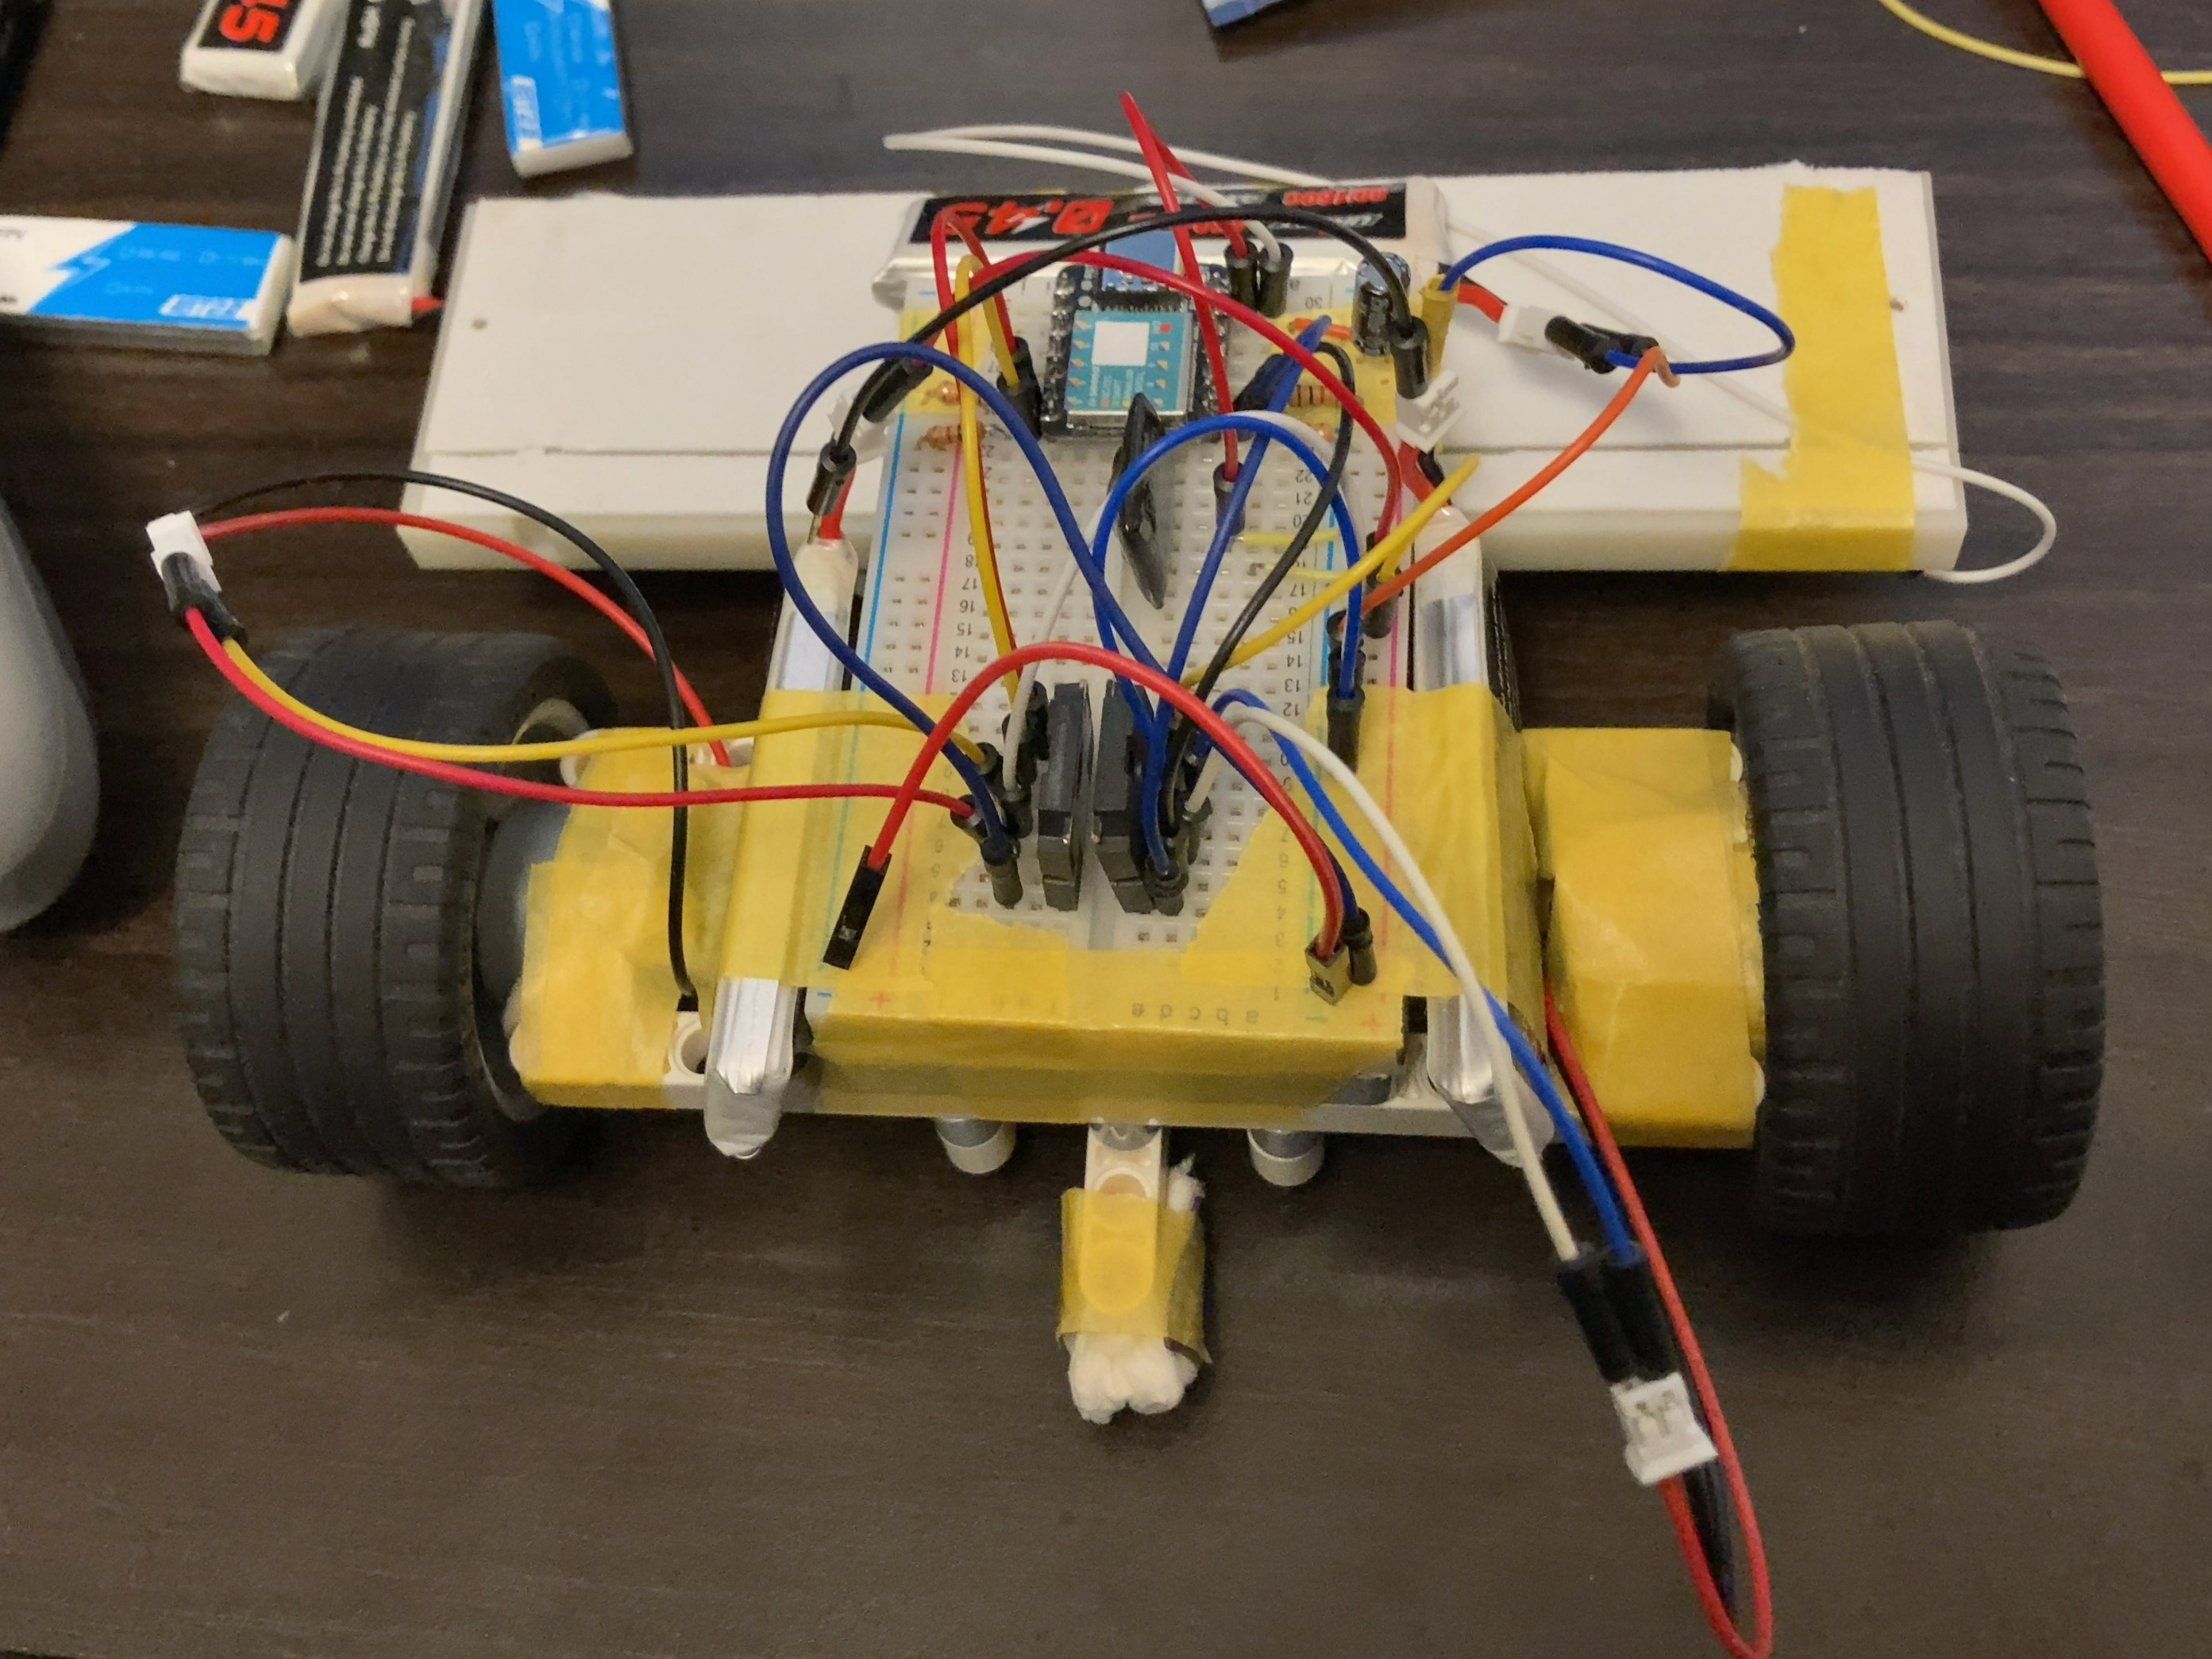
\includegraphics[keepaspectratio, scale=0.2]
       {img/beginning_machine.jpg}
  \caption{初号機}
  \label{fig:b_machine}
 \end{figure}

\section{ベースの設計}
\subsection{Version 1}
初期には本年のコースはなかったので、昨年のコースに合わせた設計(図\ref{fig:v1_machine})。
結論から言うと、今年のコースは遥かに去年のものより難しく、物理的に曲がり切ることができない設計であったためボツになった。
この設計は高速走行を目指してホイールベースが大きめ\footnote{前輪がないのでこの用法は厳密には誤りなのかもしれないが、ここではセンサ下の接地部分と後輪間の距離をホイールベースと書いている。}に作られていたほか、横幅もゆとりがあった。
高速で走る走行体はセンサが車輪から遠いほど必要な回転量が減るので有利であることでこのような設計となっていたが、今年のコースの急なカーブに対応できず、改善が求められた。


\begin{figure}[bth]
  \centering
  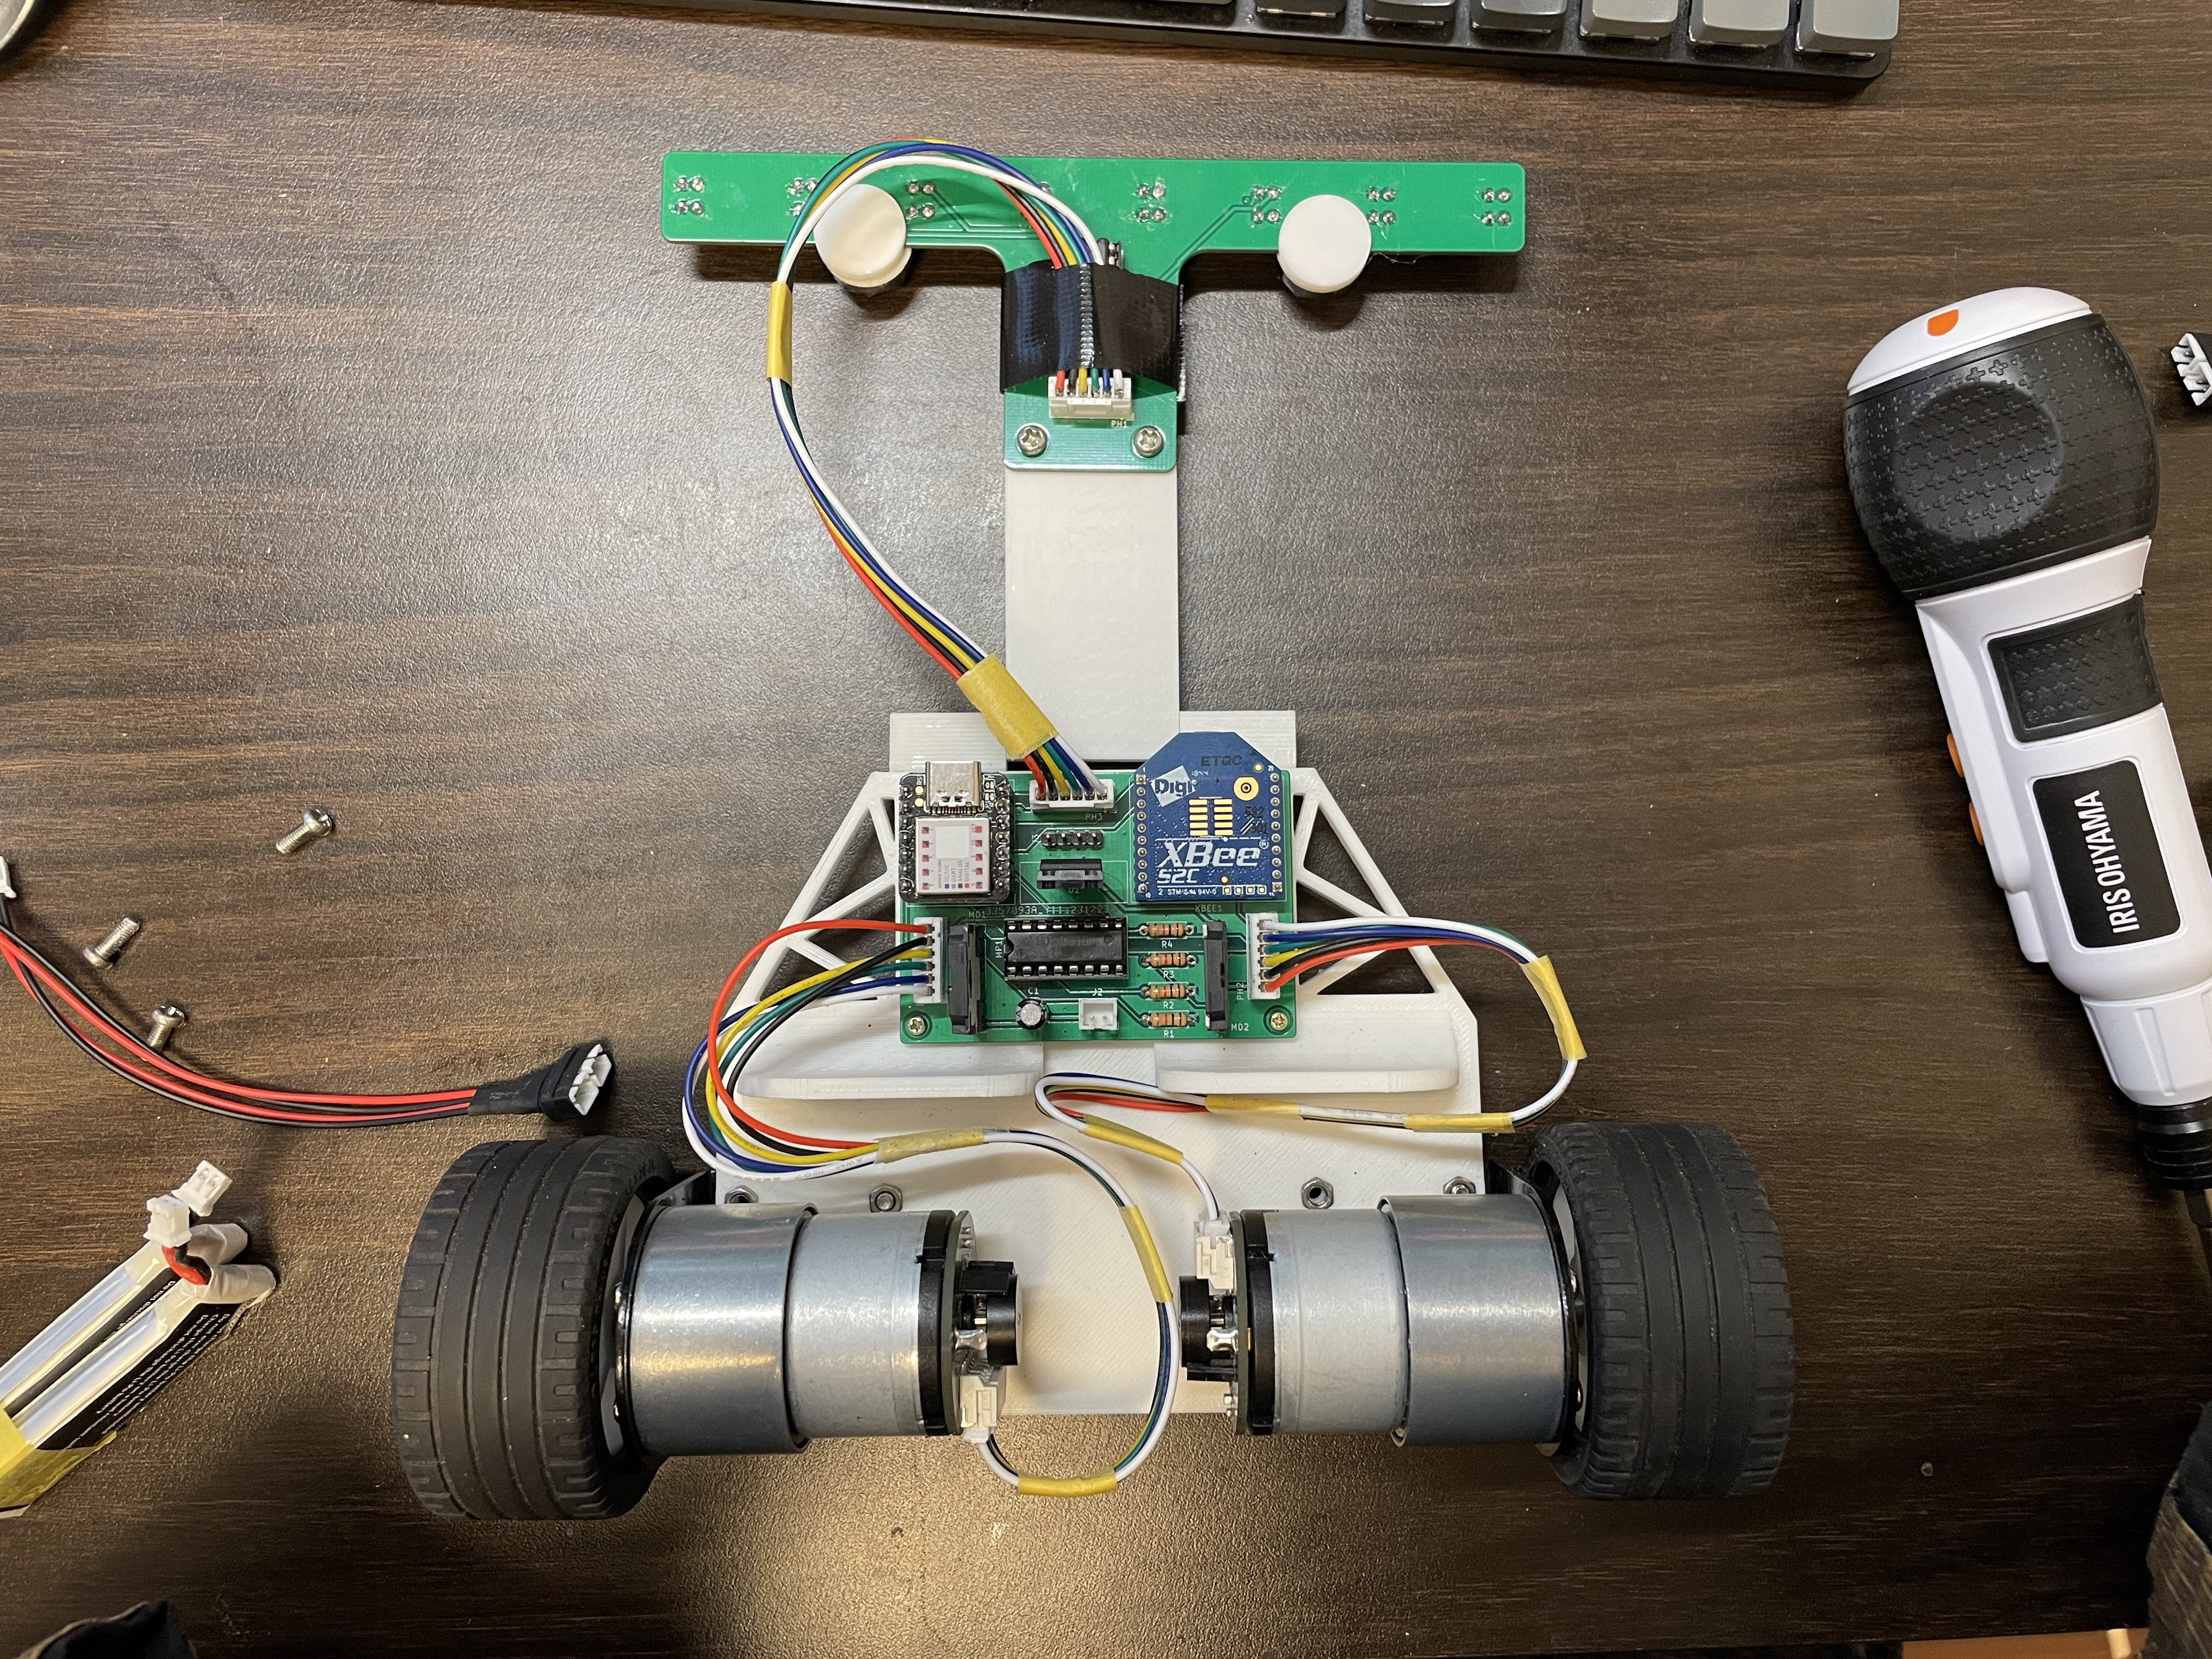
\includegraphics[keepaspectratio, scale=0.11]
       {img/ver1_machine.jpg}
  \caption{ベース Version 1を採用した機体}
  \label{fig:v1_machine}
 \end{figure}

\subsection{Version 2}
最終的に採用された設計。本編で解説した通りのものである。
ホイールベース、横幅ともに限界まで縮め、旋回性能を上げた。
\begin{figure}[bth]
  \centering
  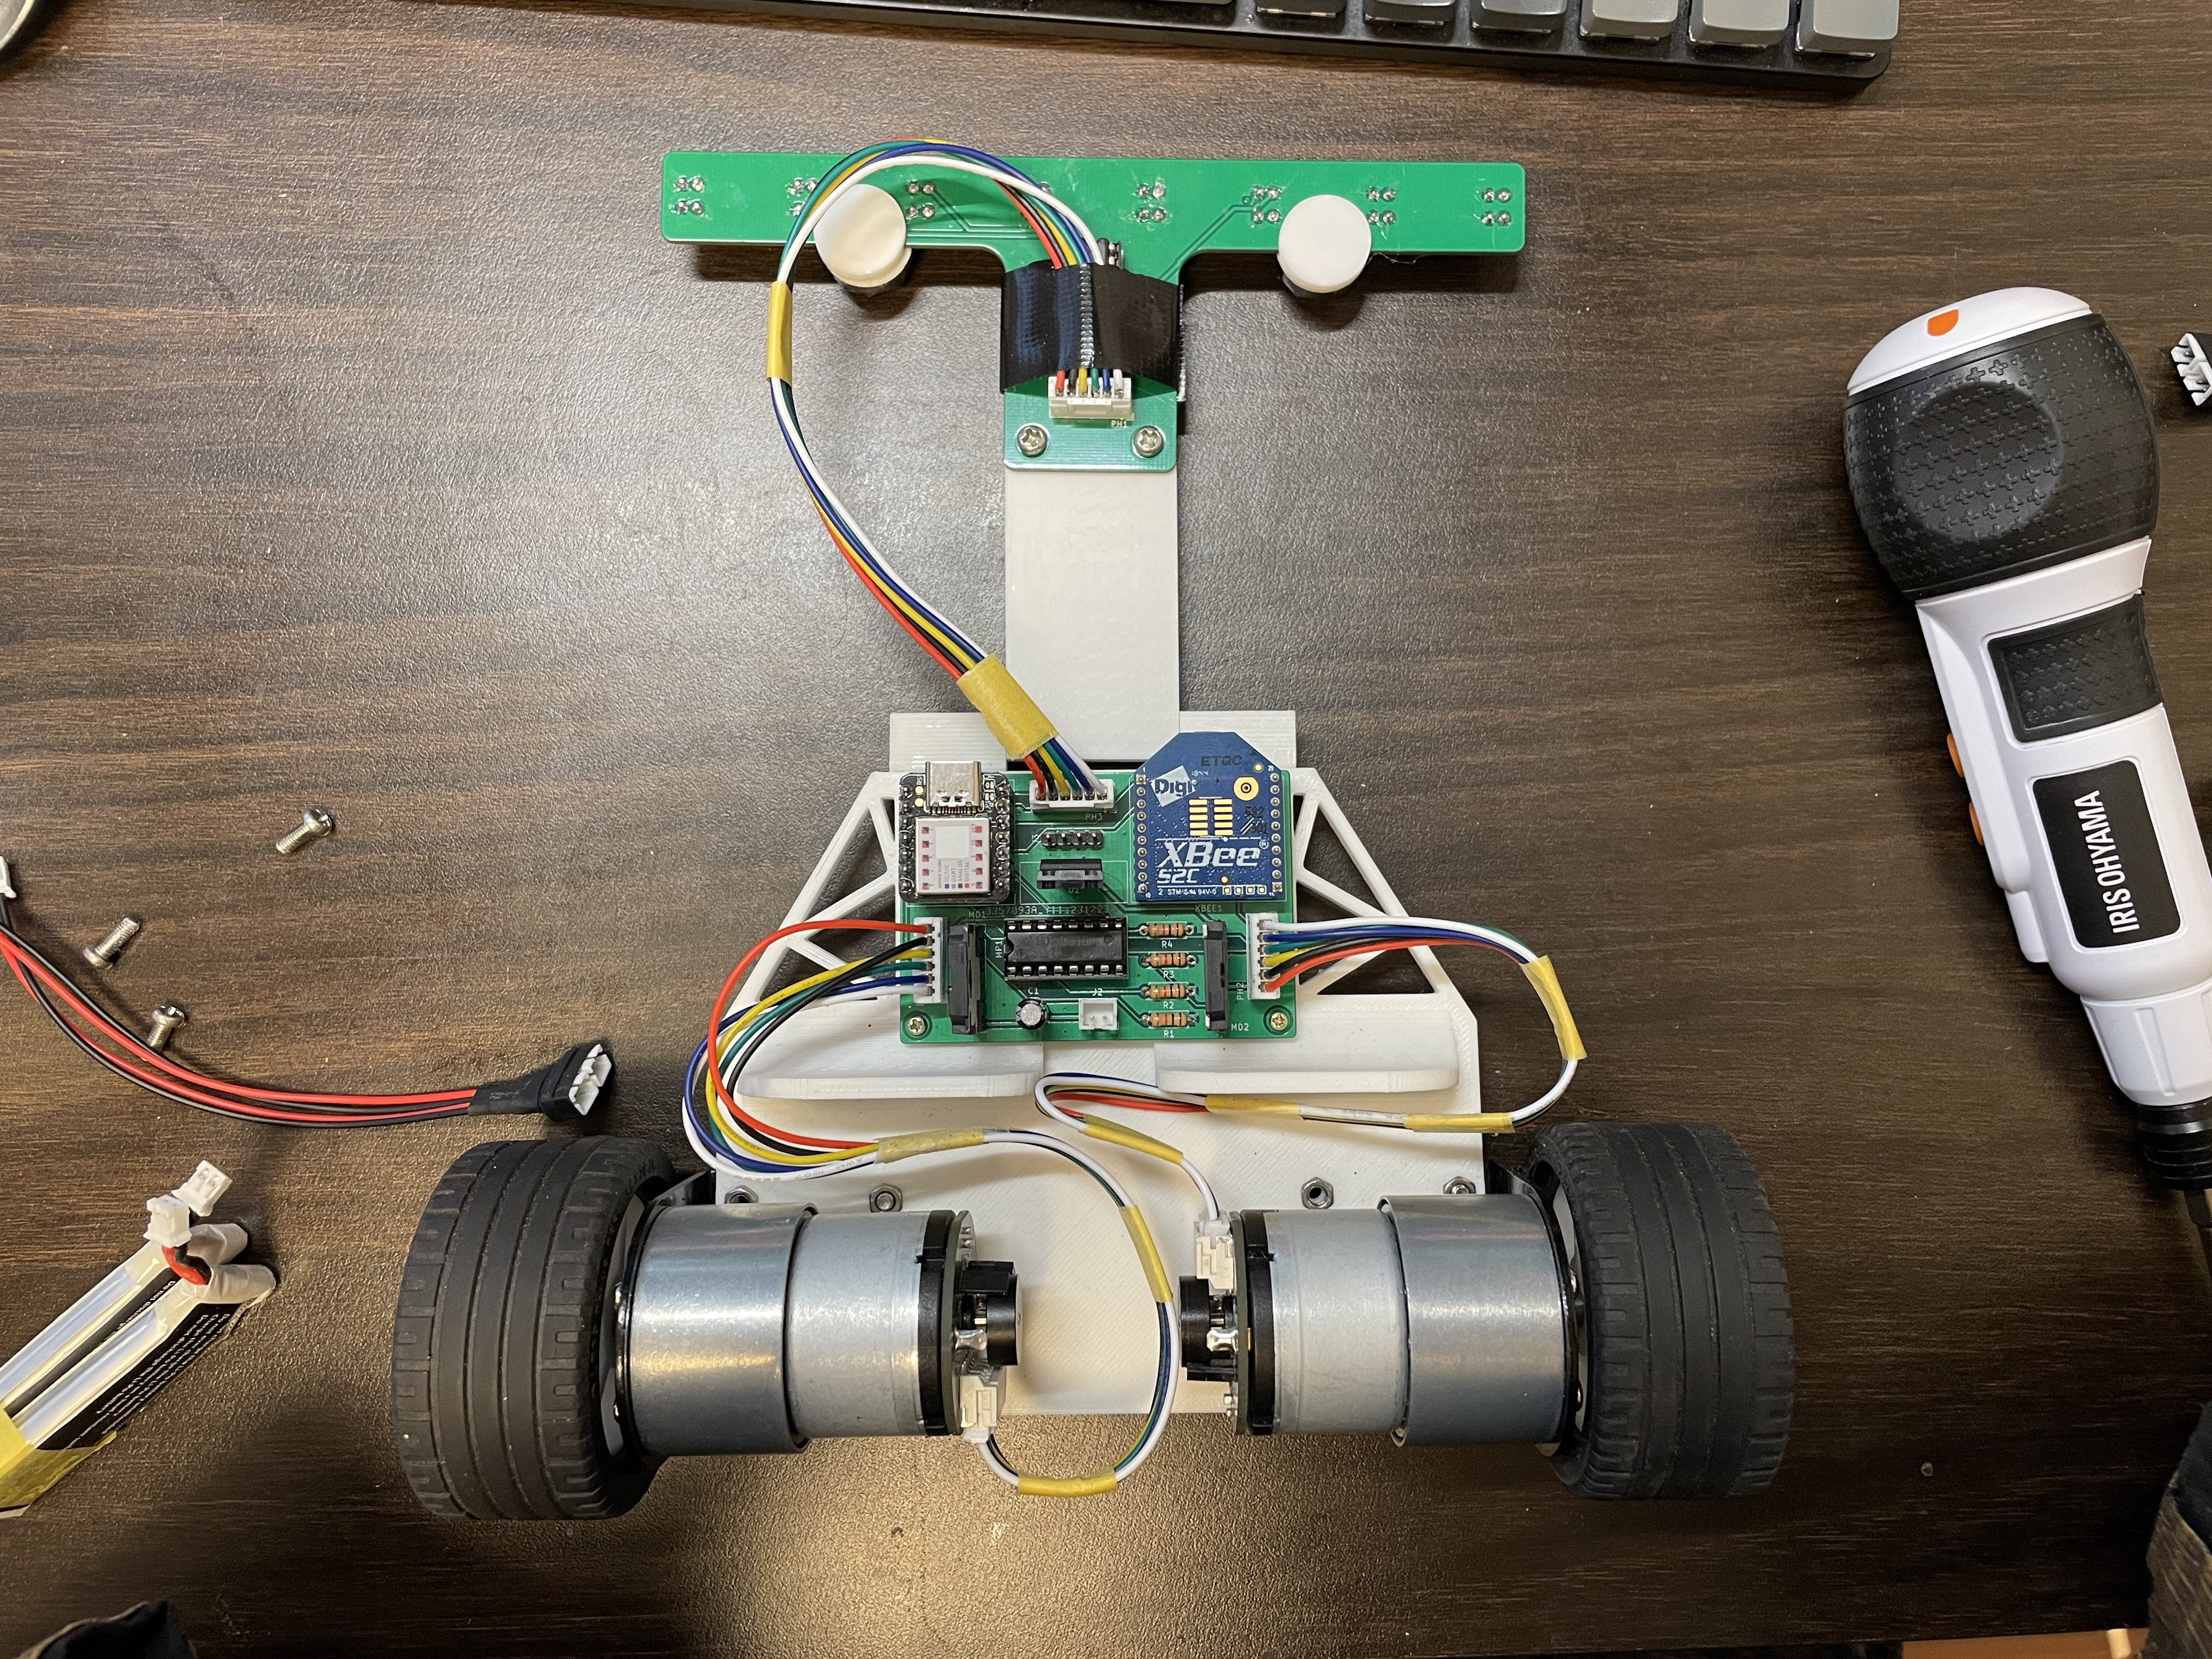
\includegraphics[keepaspectratio, scale=0.11]
       {img/ver1_machine.jpg}
  \caption{ベース Version 2を採用した機体}
  \label{fig:v2_machine}
 \end{figure}


\section{メイン基板}
\subsection{Version 1}
最初に発注した基板。
ピンアサインに問題があったので作り直しになった。

\subsection{Version 2}
問題を修正し、ついでにパーツの配置を変えることで小型化した。

%TODO: 画像入れたい

\subsection{Version 3}
プリント基板自体が変更されたわけではないが、
マルチプレクサを使わない設計に変更する必要が出てきたためユニバーサル基板で設計を少し拡張した。

\section{センサ値の統合}
\subsection{Version 1}
各センサ$i$に単純な重み$w(i) = -4+i(0\leq i \leq 3),\; -3+i (4 \leq i \leq 7)$を乗算し、単純に総和をとることで統合した。
原因はこの時点でははっきりしていなかったが、コースアウトすることが多かったため、改善に乗り出した。

\subsection{Version 2}
各センサの重みを車軸から見込んだ角度に変更した。
センサ中心からの距離と$\arcsin$を用いた実装であった。
多少改善が見られたが、振動が収まらなかった。

\subsection{Version 3}
最終的に採用されたシステム。
重み付けして総和を出すのではなく、コース線の中心を推定することで単調性を確保し、
安定したターンを実現した。
角度を求める関数も三平方の定理が必要ない$\arctan$に変更され、計算量が減少した。





\chapter{インシデント、問題解決集}
\section{概要}
ロボット製作をしていると、原因不明の問題が次々と発生し、時間がどんどん吸い取られていくことがよくある。
本章では、開発中に実際にあったハマりどころを列挙し、原因を述べる。


\section{レギュレータの周波数特性}
当初使用していたDC-DCレギュレータは高級な作りになっていて、レギュレータという名前にもかかわらず、コンバーダのような仕組みだった。その結果、モーターが回転し始めた瞬間の過渡現象的な電源の電圧降下を拾ってしまい、5V出力のレギュレータが瞬間的に2V程度になりマイコンが落ちてしまうという問題が発生した。電源側は12V程度供給していて、電圧降下したときも9V程度を維持していたからレギュレータ側に問題があると気づくのに遅れた。
コンデンサで安定化させ、レギュレータをシンプルな3端子レギュレータに変更することで解決した。

\section{PHコネクタ接触不良}
よくある話から。
本機では、PHコネクタを用いていくつかの配線を束ねていたが、1本だけ接触が悪いという状況は案外気づきにくく、「力を加えると精度が向上する」などと呼ばれていた。

\section{回路設計のミス}
発注した基板の設計ミス。本来電源が供給されるべきところであるのに、浮島となっていて0Vとなっているところがいくつかあった。基板表面を削って適当に電源が供給されているところとはんだ付けすることで解決した。

また、センサの基板で表裏を間違えていて、フォトセンサの素子の向きを全部直さないといけなくなった。

\section{マイコンのバグ}
マイコンにプログラム書き込んで、そのまま使用すると8番ピンの出力電圧が不安定になるというバグ。
書込み後、一度電源と切り離し、再度電源と接続すると問題なく動作するため再現が難しく、ことあるごとに悩まされた。
個体差なのか仕様なのかは定かでない。

\section{温度特性}
教室では良好に動いていたのに、家に持ち帰り確認すると全く違う値が出る。いったい何が違うのだろう?
その答えは素子の温度特性。寒い外気にさらされて持ち帰ってきた機体は、抵抗器も半導体素子も別の特性を示すのである。
現実の素子がいかに理想的でないか思い知らされる出来事である。

\section{何もしてないのに壊れた}
一度も使用していなかったマルチプレクサが、正しく動作していなかった。
初期不良か、静電気か。

\section{テスタの個体差}
大きなプルアップ抵抗を使用していると、電圧を測ったとき、テスタ側の内部抵抗によって分圧され、思ったのと違う値になる。
普通の回路では気にならないが、\SI{1}{\Mohm}の抵抗を使用していたため、テスタの内部抵抗と同じくらいのオーダになっていたようだ。
安物のテスタでは2.1 V を示し、もっと良いテスタでは3.5 Vということが起こり、再現性の無さに苦労した。

\section{これらの組み合わせ}
これらの問題が独立に発生しているなら、まだ苦労しなかっただろう。
しかし、2つまとめて起こる、ということが頻発したため非常に苦労した。

\chapter{ソースコード} \label{cha:code}
\lstinputlisting[caption = main.ino  , style=c++]{code/main.ino}
\lstinputlisting[caption=sensor.ino, style=c++]{code/sensor.ino}



\end{document}